\documentclass[12pt,a4paper]{report}
\usepackage[utf8]{inputenc}
\usepackage[T1]{fontenc}
\usepackage{fontspec}
\usepackage[polish]{babel}
\usepackage{amsmath}
\usepackage{graphicx}
\usepackage{mathtools}
\usepackage[table,xcdraw,dvipsnames]{xcolor}
\usepackage{hhline}
\usepackage{placeins}
\usepackage[margin=0.6in]{geometry}
\usepackage{appendix}
\usepackage{colortbl}
\usepackage{physics}
\usepackage{float}
\usepackage{caption}
\usepackage{subcaption}
\usepackage{datetime}
\usepackage{makeidx}
\usepackage{hyperref}
\usepackage{amsfonts}
\usepackage{fancyhdr}

\title{Termodynamika R 2021/2022}
\author{Kacper Cybiński}
% \newdate{date}{28}{01}{2022}
% \date{\displaydate{date}}
\date{\today}
\makeindex
\setlength\parindent{0pt}

\addto\captionspolish{\renewcommand{\chaptername}{Wykład}}

\newcommand{\ind}[1]{{\color{blue} #1\index{#1}}}

\newcommand{\subind}[2]{{\color{blue} #1\index{#2}}}

\newcommand{\com}[1]{{\color{red} #1}}

\newcommand{\link}[2]{{\color{cyan} \href{#1}{#2}}}

\renewcommand{\emph}{\textbf}

\newcommand{\linediv}{{\color{RubineRed} \rule{\linewidth}{0.5mm}}}

\newcommand{\wniosek}{{\color{orange} Wniosek:}}

\newcommand{\dbar}{d\hspace*{-0.08em}\bar{}\hspace*{0.1em}}

\newenvironment{lecture}[1]{\par\medskip
   \noindent\chapter{#1} \rmfamily}{\medskip}
   
\newenvironment{emph_box}[1]
    {\begin{center}
    \begin{tabular}{|p{0.9\textwidth}|}
    \hline
    \begin{center} \textbf{#1} \end{center}\\[1ex]
    }
    { 
    \\\\\hline
    \end{tabular} 
    \end{center}
    }
    
    
\pagestyle{fancy}
% zmiana liter w~żywej paginie na małe
\renewcommand{\chaptermark}[1]{\markboth{#1}{}}
\renewcommand{\sectionmark}[1]{\markright{\thesection\ #1}}
\fancyhf{} % usuń bieżące ustawienia pagin
\setlength{\headheight}{15pt}
\fancyhead[LE,RO]{\bfseries\thepage}
\fancyhead[LO]{\bfseries\rightmark}
\fancyhead[RE]{\bfseries\leftmark}
\renewcommand{\headrulewidth}{0.5pt}
\renewcommand{\footrulewidth}{0pt}
\addtolength{\headheight}{0.5pt} % pionowy odstęp na kreskę
\fancypagestyle{plain}{%
\fancyhead[LE,RO]{\bfseries\thepage} % usuń p. górne na stronach pozbawionych
% numeracji (plain)
\renewcommand{\headrulewidth}{0.5pt} % pozioma kreska
}

\begin{document}

\maketitle

% ---------------------------------------------------------------------------
% Wykład 01.03.2022

\chapter*{Organizacja wykładu}
\begin{enumerate}
    \item Dwa kolokwia - po 40 \% pkt
    \item Zadania domowe - 20 \% pkt
\end{enumerate}

{\color{blue} \link{http://www.fuw.edu.pl/~piotrek/stat2022}{Strona wykładu}}

Suma - 100 \%. Zaliczenie ćwiczeń $> 50 \%$, Egzamin 100 \%. Propozycja oceny w zakresie $3-4.5$ Po 5 przychodzimy na ustny. Ustny też dla plebsu, nie tylko dla tych z 4.5 ({\it Patrz Pawełczyk})

Egzamin i kolokwia mają 2 częsci:
\begin{itemize}
\item Test ABCD, 1 lub wielokrotnego wyboru $\sim 45$ min.
\item Zadania - $\sim 3h$
\end{itemize}

Zadania domowe: Jak na elektro, ale tylko 3 zadania na tydzień. Na wykładzie czwartkowym losowanie zadania zbieranego. Jest jedno dodatkowe, trudniejsze, "Joker".

\begin{lecture}{Wstęp, Ergodyczność}
\section{\ind{Problem wielu ciał}}

Dla problemu 3 ciał pierwsze znalezione stabilne rozwiązanie zostało opisane przez Lagrange'a. Jest to ruch po okręgu, a w $\sim 1990$ opisano też stabilną orbitę po ósemce.

Historia superkomputerów:
\begin{itemize}
    \item Anton (2008) - Daniel Shaw
    \begin{itemize}
        \item Problem zwijania białek
        \item 10 ms zwijania - 5 min obliczeń
        \item $10^4-10^5$ atomów - 1 ms w 100 dni. Tj. $10$ ns/dzień
    \end{itemize}
    \item Summit (2018)
    \begin{itemize}
        \item 27 tys. GPU + 9 tys. CPU.
        \item $200\cdot10^6$ 32 ns/dzień
    \end{itemize}
\end{itemize}
Dla skali -> kubek z herbatą ma \textbf{$\sim10^{25}$ atomów}

\ind{Demon Laplace'a}:
Laplace mówił, że symulacja, która by znała położenia i pędy wszyskich cząstek by znała przeszłość i przyszłość $\to$ \textit{przeszłość i przyszłość by stała przed nią otworem}. Jest to wizja świata skrajnie deterministycznego. Obecnie raczej upadłej. \wniosek Kupując kefir nie obchodzi nas położenie wszystkich atomów, a właściwości makroskopowe.

\ind{Fizyka statystyczna}: Jest dziedziną zajmującą się przejściem z informacji mikroskopowej do informacji makroskopowej, która jest obiektem naszego zainteresowania.

\begin{figure}[!ht]
    \centering
    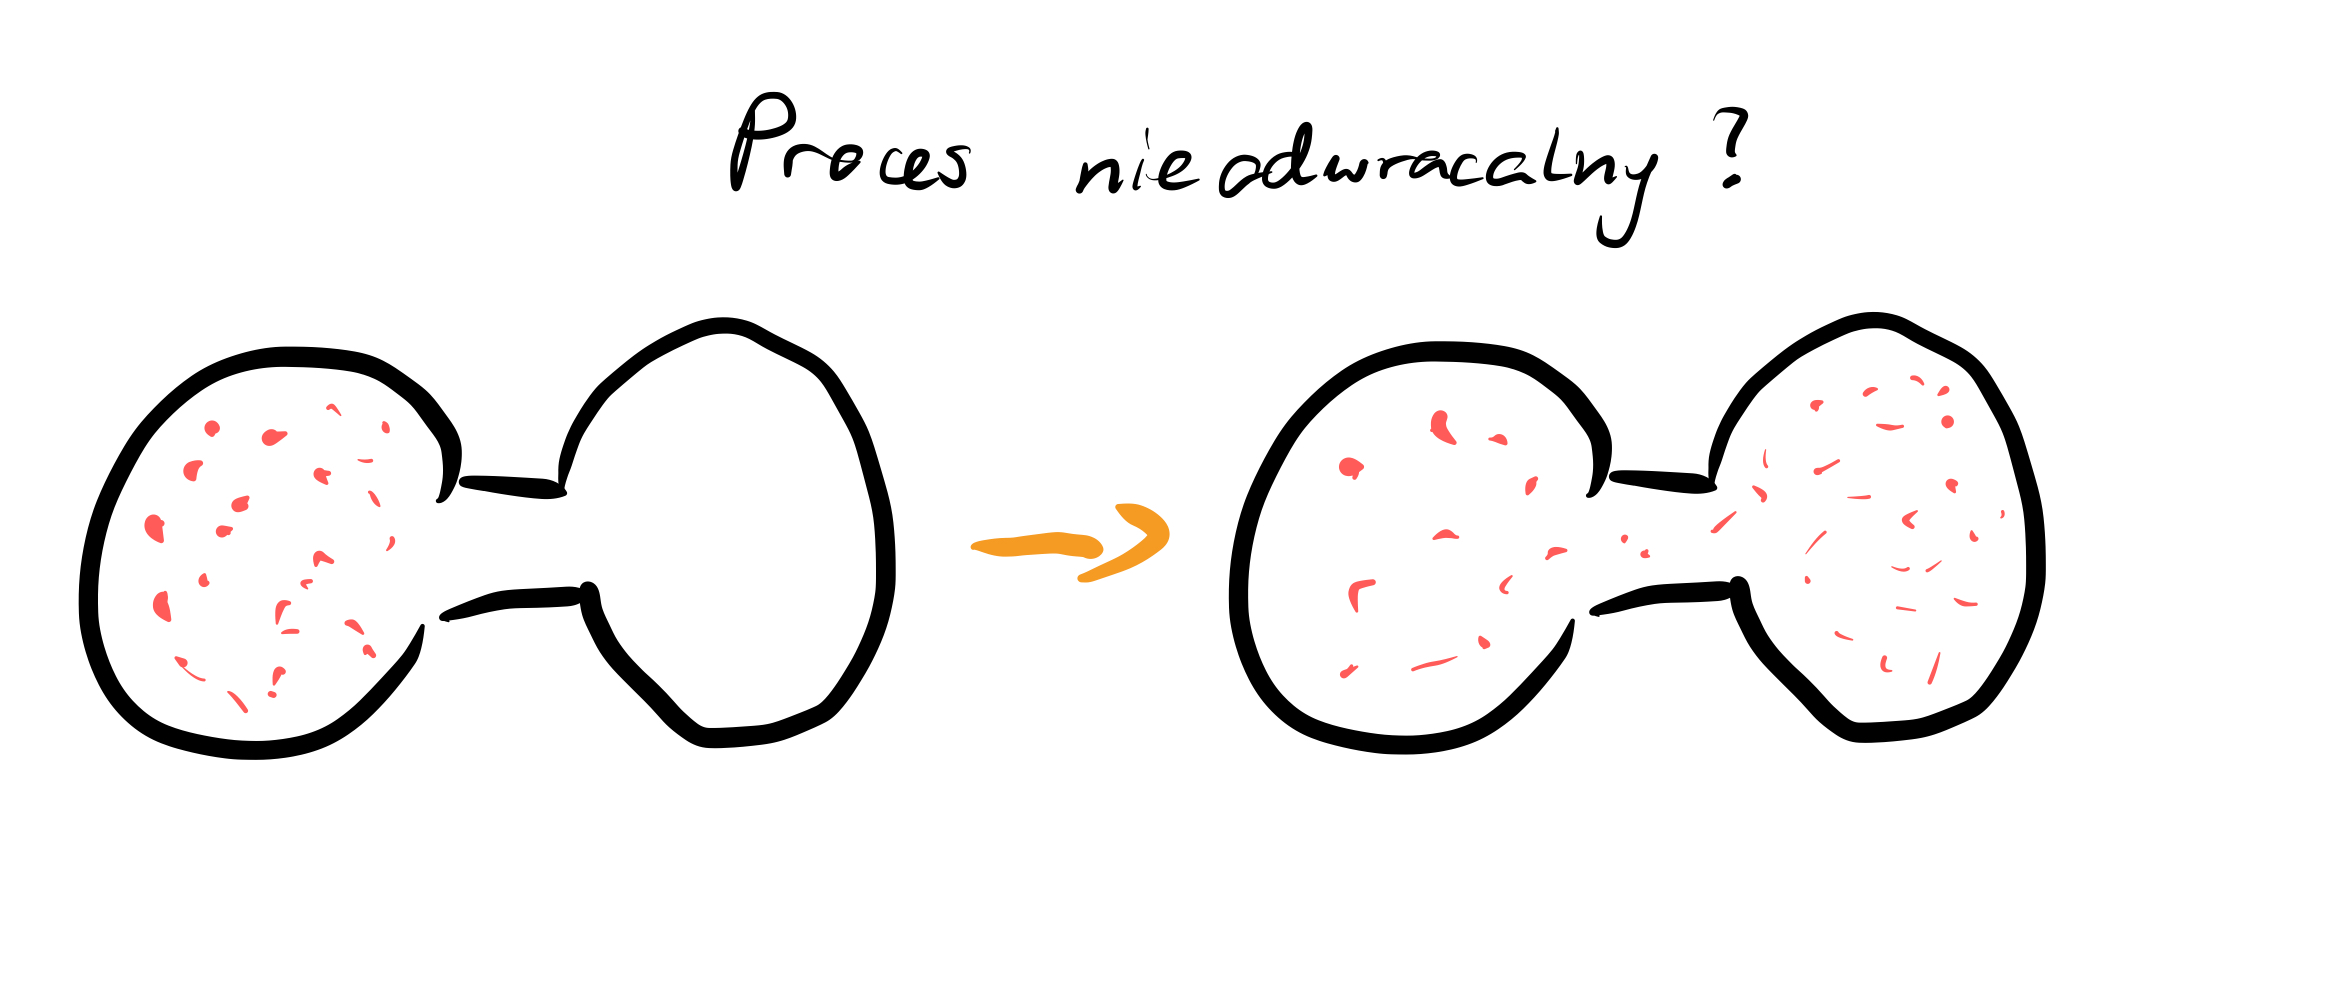
\includegraphics[width=0.8\linewidth]{Wyk_1_Rys_1.jpeg}
    \caption{Proces nieodwracalny?}
\end{figure}

\FloatBarrier

\section{Pokazy}
\subsection{Cylindry z ulepkiem cukru}
Widzimy tu na demonstracji \ind{odwracalność}. Są dwa rodzaje:
\begin{itemize}
    \item {\color{blue} odwracalność dynamiczna} \index{odwracalność!dynamiczna}:
    \[m \dv{v}{t} = F\]
    Wynika ona z dynamiki Newtonowskiej, jest symetryczna względem transformacji $t \to -t$, $v \to -v$.
    \item {\color{blue} odwracalność kinematyczna} \index{odwracalność!kinematyczna}:
    \[0 = m \dv{v}{t} = F - \gamma v \implies v = \frac{F}{\gamma}\]
    Gdzie $\gamma$ jest współczynnikiem oporu. Ta odwracalnośc jest symetryczna względem przekształcenia $F \to -F, v \to -v$. Ten rodzaj odwracalności zachodzi w lepkich cieczach. Symetryczny względem zmiany kierunku siły i prędkości, ale z czasem nieodwracalnym.
\end{itemize}

\begin{figure}[!ht]
    \centering
    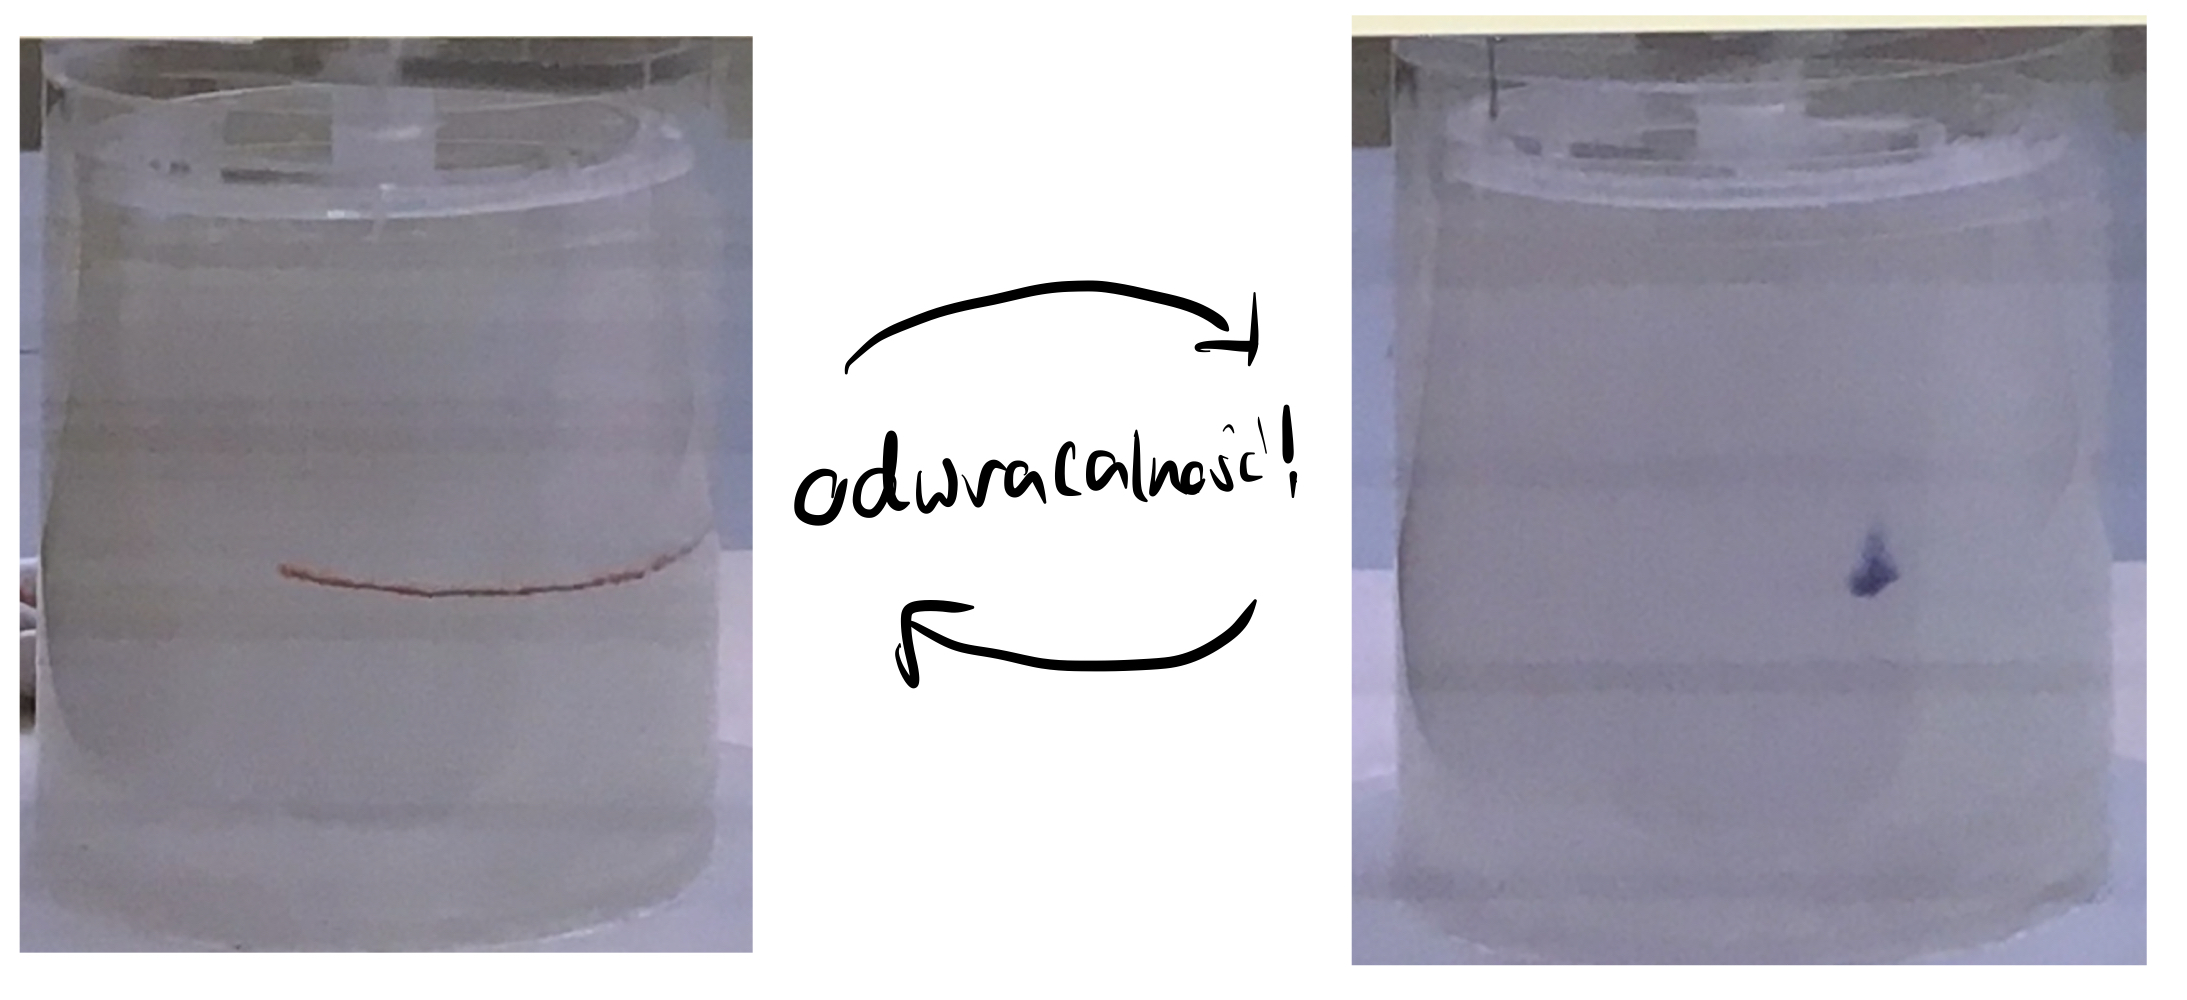
\includegraphics[width=0.8\linewidth]{Wyk_1_Rys_2.jpeg}
    \caption{Demonstracja odwracalności kinematycznej. Działa to tylko dla \emph{lepkiej cieczy}}
    \label{fig:lec_1:odwracalność}
\end{figure}

\begin{figure}[!ht]
    \centering
    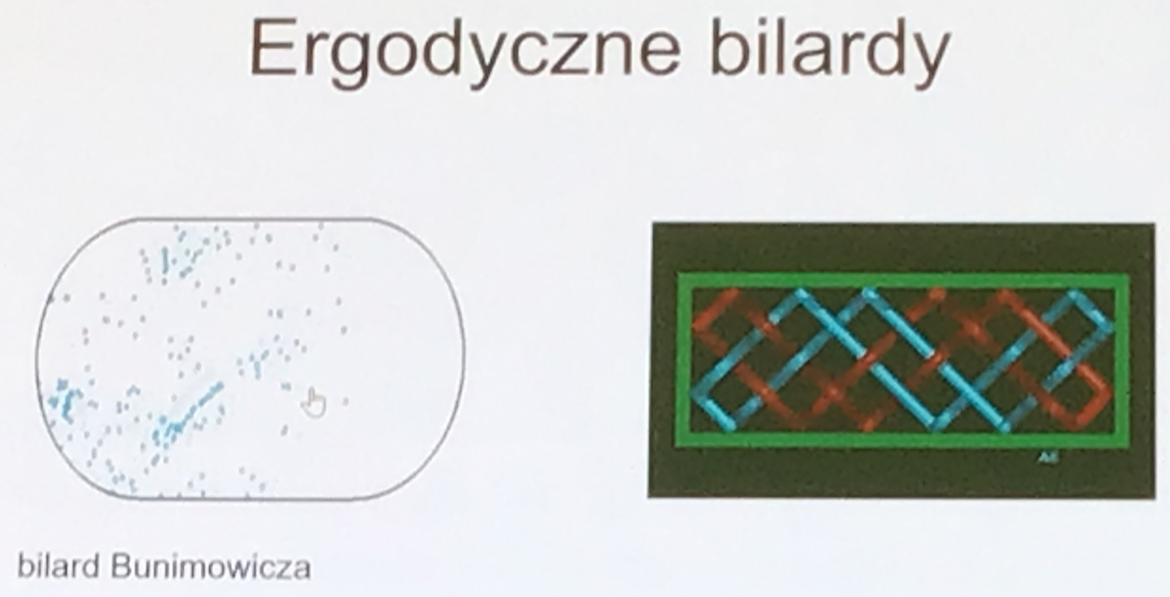
\includegraphics[width=0.8\linewidth]{Wyk_1_Rys_3.jpeg}
    \caption{Demonstracja \emph{Bilardu Bunimowicza}. Po prawej bilard prostokątny - Nie Ergodyczny, ponieważ po odpowiednio długim czasie nie uśrednia się rozkład cząstek - Nie osiąga równowagi.}
    \label{fig:lec1:bilardbunimowicza}
\end{figure}

Kolejnym pojęciem które się pojawia jest \ind{ergodyczność}. Oznacza to, że średnia $\expval{x}$ z układu  po czasie jest równa średniej po powierzchni. Przykładem takiego układu jest zasadniczo \emph{Bilard bunimowicza} (Patrz Rysunek \ref{fig:lec1:bilardbunimowicza}). Układ ergodyczny to taki, który po odpowiednio dużym czasie osiąga stan równowagi.


\section{Model Ehrenfestów}
\begin{figure}[!ht]
    \centering
    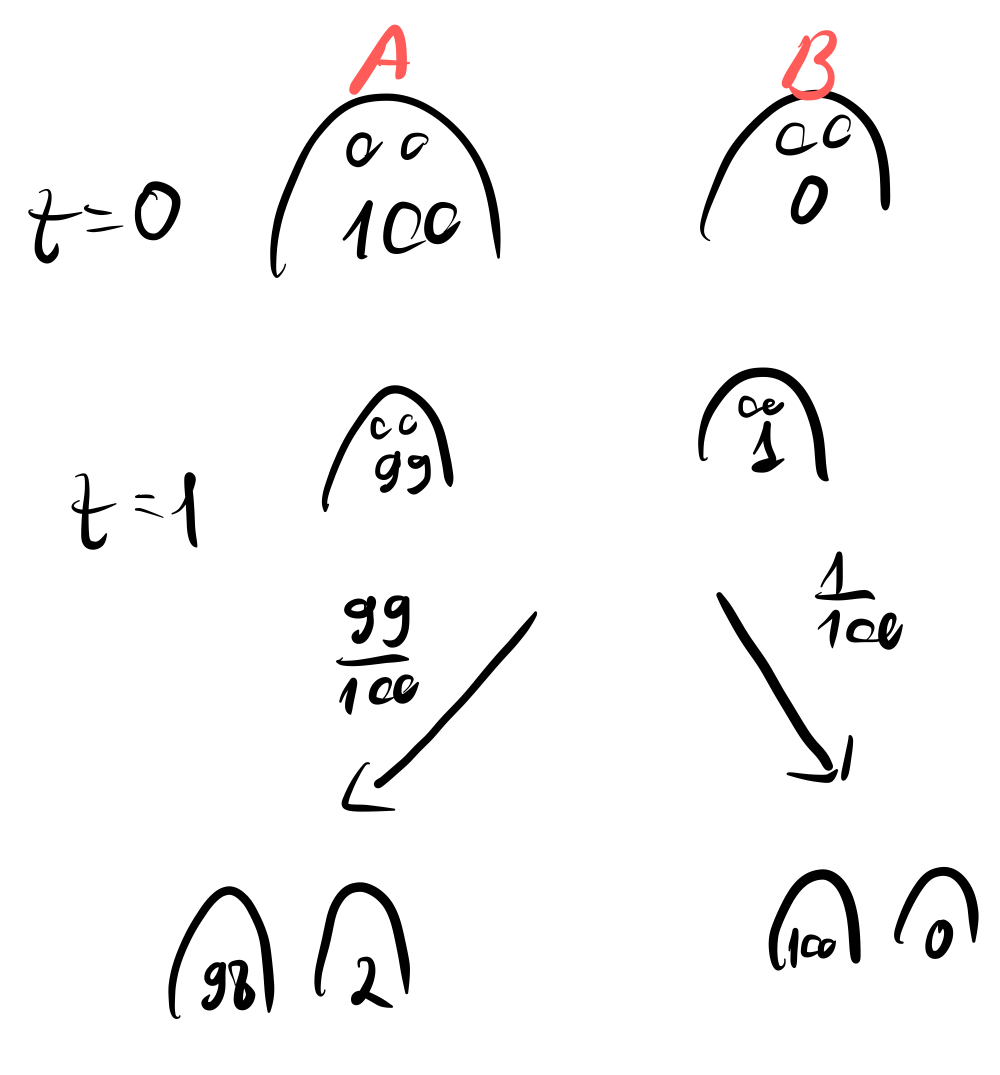
\includegraphics[width=0.8\linewidth]{Wyk_1_Rys_4.jpeg}
    \caption{Demonstracja \emph{Modelu Ehrenfestów}. Bierzemy dwa psy i liczymy sobie $\expval{n_a(t)}$. W tym celu patrzymy sobie na \ind{ansambl} (zespół) dwójek psów.}
    \label{fig:lec_1:pchły}
\end{figure}

\end{lecture}

% --------------------------------------------------------------------------
% Wykład 03.03.2022

\FloatBarrier

\begin{lecture}{Ruchy Browna, Równanie Master}
\section{Ruch cząstek - Ruchy Browna}

Wprowadzamy sobie jak propaguje się cząstka w cieczy w czasie.

\begin{figure}[!ht]
    \centering
    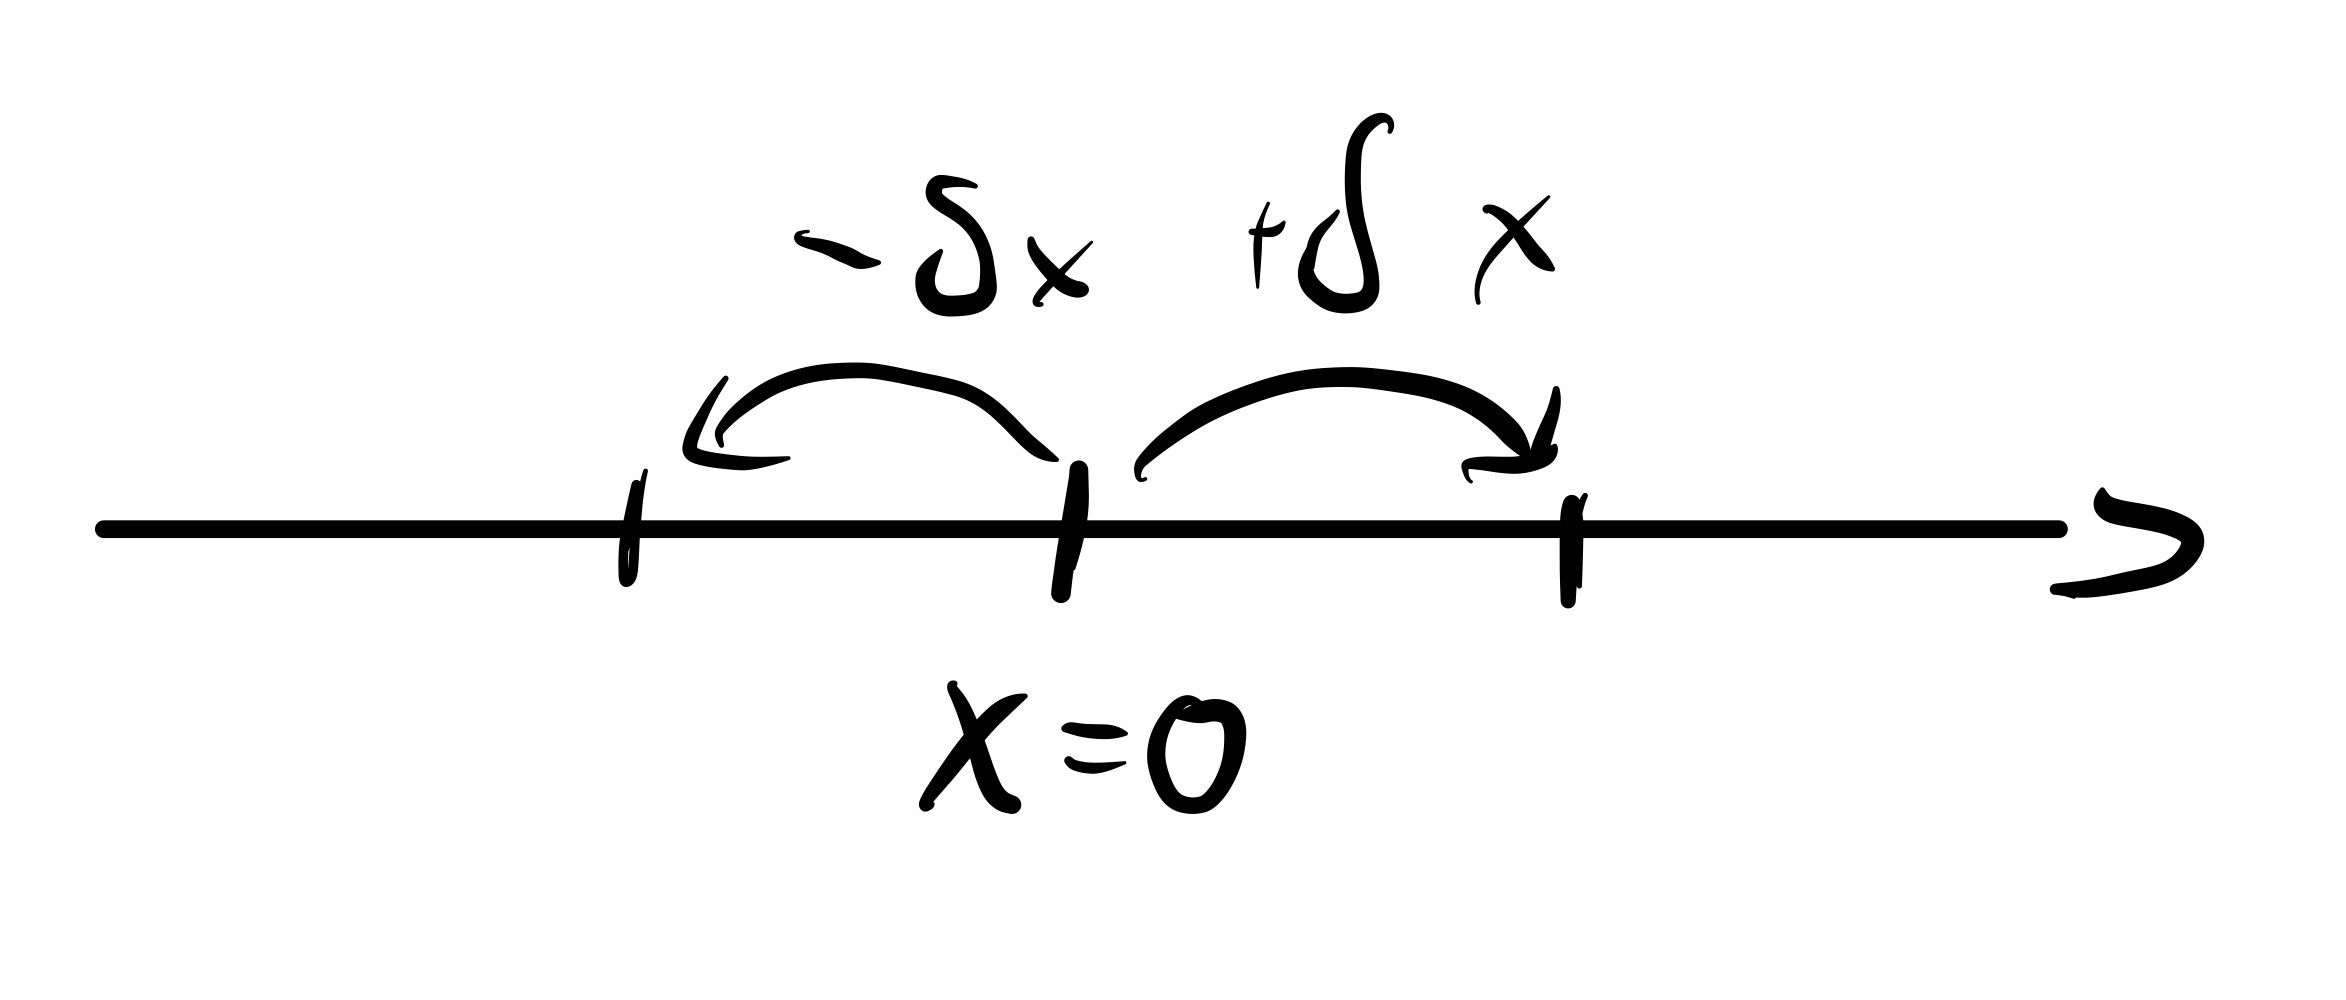
\includegraphics[width=0.8\linewidth]{Wyk_2_Rys_1.jpeg}
    \caption{Położenie cząstki}
    \label{fig:lec_2:czastka}
\end{figure}

Skoki o $\delta x$ następują co $\delta t$ i mamy:
\[ \Delta x = \begin{cases}
    \delta x \qc \frac{1}{2} \\
    - \delta x \qc \frac{1}{2}
\end{cases}\]

\begin{align*}
    x(n) = x(n-1) + \Delta x\\
    \expval{x(n)} = \expval{x(n-1)} = \expval{x(n-2)} \dots = \expval{x(0)} = 0
\end{align*}

Wynika, że:
\begin{align*}
    x(n)^2 = (x(n-1) + \Delta x)^2 = x^2(n-1) + 2x(n-1)\Delta x + (\Delta x)^2\\
    \expval{x^2(n)} = \expval{x^2(n-1)} + 2\expval{x(n-1)\Delta x} + \expval{(\Delta x)^2}
\end{align*}

Gdzie wiemy, że $2\expval{x(n-1)\Delta x} = 0$  bo kolejne skoki są niezależne, a $\expval{(\Delta x)^2} = (\delta x)^2$

Czyli:
\begin{align*}
    \expval{x^2(n)} = \expval{x^2(n-1) + (\delta x)^2}\\
    \expval{x^2(n)} = n (\delta x)^2 + \expval{x^2(0)}
\end{align*}
Ale $\expval{x^2(0)} = 0$, więc widzimy, że:
\[
    \expval{x(n)} = 0 \qc \expval{x^2(n)} = n (\delta x)^2
\]
Teraz oznaczmy sobie $n = \frac{T}{\delta t}$, a $\frac{(\delta x)^2}{2 \delta t} = D$ - stała dyfuzji. Wtedy dostajemy ruch dyfuzyjny (\ind{Ruch Browna}).
\[
    \expval{x^2(n)} = 2 T \frac{(\delta x)^2}{2 \delta t}
\]
Dokładna definicja ruchu Browna to:
\[
    \text{ruch Browna} = 
    \begin{cases}
    \expval{x^2(n)} = 2 D T \\
    \expval{x(n)} = 0
    \end{cases}\qq{gdzie}
    x = vt\qc t=\frac{L}{v}\qc T=\frac{L^2}{2D}
\] gdzie $L$ - odległość.

Przykładowe wartości:\\
\emph{Bakteria} - $L \sim 10^{-4}$ wtedy $D \sim 10^{-5} \frac{cm^2}{s}$ a czas dyfuzji $t = \frac{L^2}{2 D} = 5 \cdot 10^{-4} \sim (0.5)\,$ms
ale np z jednogo końca auli na drugi szło by to miesiąc.\\
\emph{Takeaway} - Zapachy nie transportują się dyfuzyjnie!

\section{\subind{Równanie Master}{Równanie!Master}}

\begin{figure}[!ht]
    \centering
    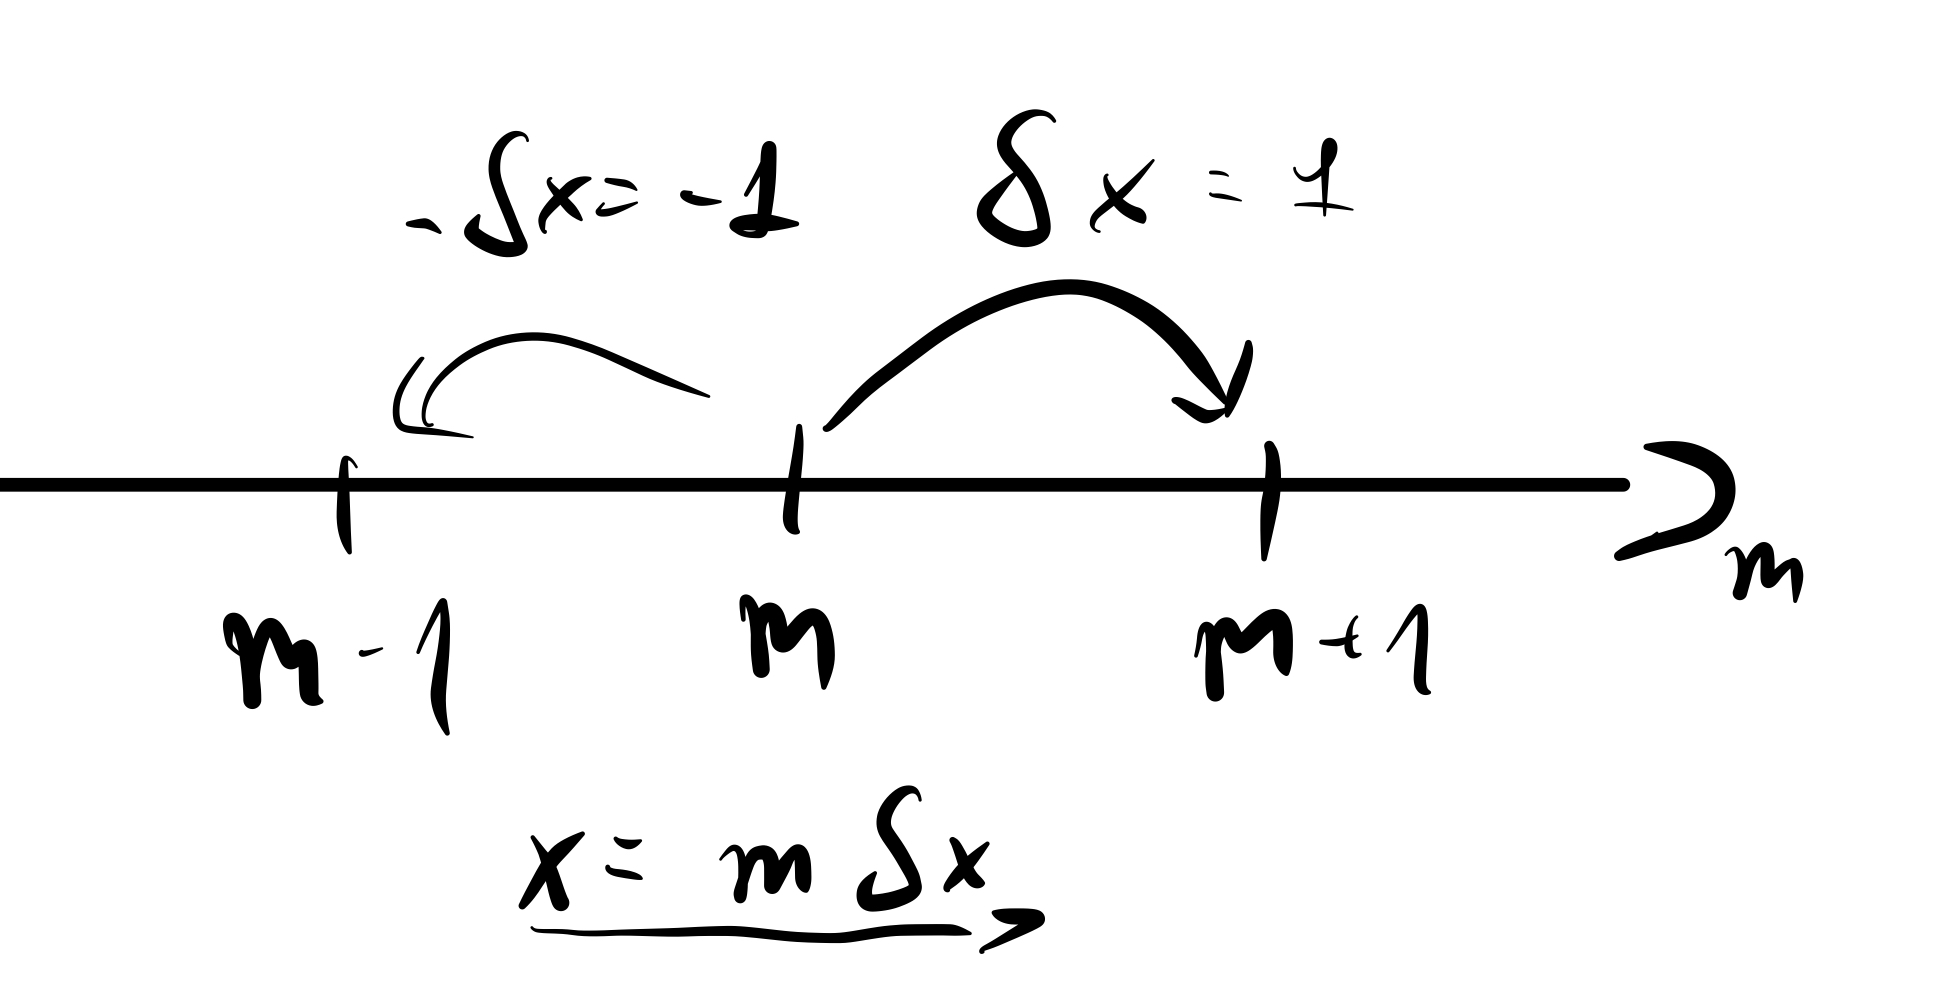
\includegraphics[width=0.8\linewidth]{Wyk_2_Rys_2.jpeg}
\end{figure}

$x = m \delta x \to$, $t \pm 1 = t \pm \delta t$

\begin{align*}
    P(m, t+1) &= \frac12 P(m+1, t) + \frac12 P(m-1, t )\\
    P(m, t+1) - P(m, t) &= \frac12(P(x + \delta x, t) - 2P(x, t) + P(x - \delta x, t))\\ 
    \qq{co jest drugą pochodną w punkcie}x:&\\
    P(m, t+1) - P(m, t) &= \frac12\delta x\qty(\frac{P(x + \delta x, t) - P(x, t)}{\delta x} - \frac{P(x, t) - P(x - \delta x, t)}{\delta x})\\
    P(m, t+1) - P(m, t) &= \frac12(\delta x)^2\qty(P'\qty(x + \frac{\delta x}{2}, t) - P'\qty(x - \frac{\delta x}{2}, t))\\
    \qq{co na mocy \textit{central limit theorem}}& \text{tłumaczy się na:}\\
    \pdv{P}{t} &= \frac{P(x, t+\delta t) - P(x, t)}{\delta t} = \frac{(\delta x)^2}{\delta t}\pdv[2]{P}{x}\\
    \qq{po przejściu do granic:} &\delta t \to 0\qc \delta x \to 0\qc \frac{\delta x^2}{\delta t} = \qq{const.}\\
\end{align*}
Dostajemy równanie dyfuzji:
\begin{equation}
    \pdv{P}{t} = D \pdv[2]{P}{x}
    \label{eq:lec_2:dyfuzja}
\end{equation}
Co dla
\[
    P(x, t=0) = \delta(x)
\]
Daje nam rozkład prawdopodobieństwa występowania punktu w jakimś $x$ przy dyfuzji wygląda:
\begin{equation}
    P(x) = \frac{1}{\sqrt{4 \pi D t}} e^{-\frac{x^2}{4 D t}}
    \label{eq:lec_2:rozklad_gauss}
\end{equation}
Czyli rozkład Gaussa, widoczny na Rysunku \ref{fig:lec_2:mol_pow}.

\section{Demonstracje}
\begin{figure}[!ht]
    \centering
    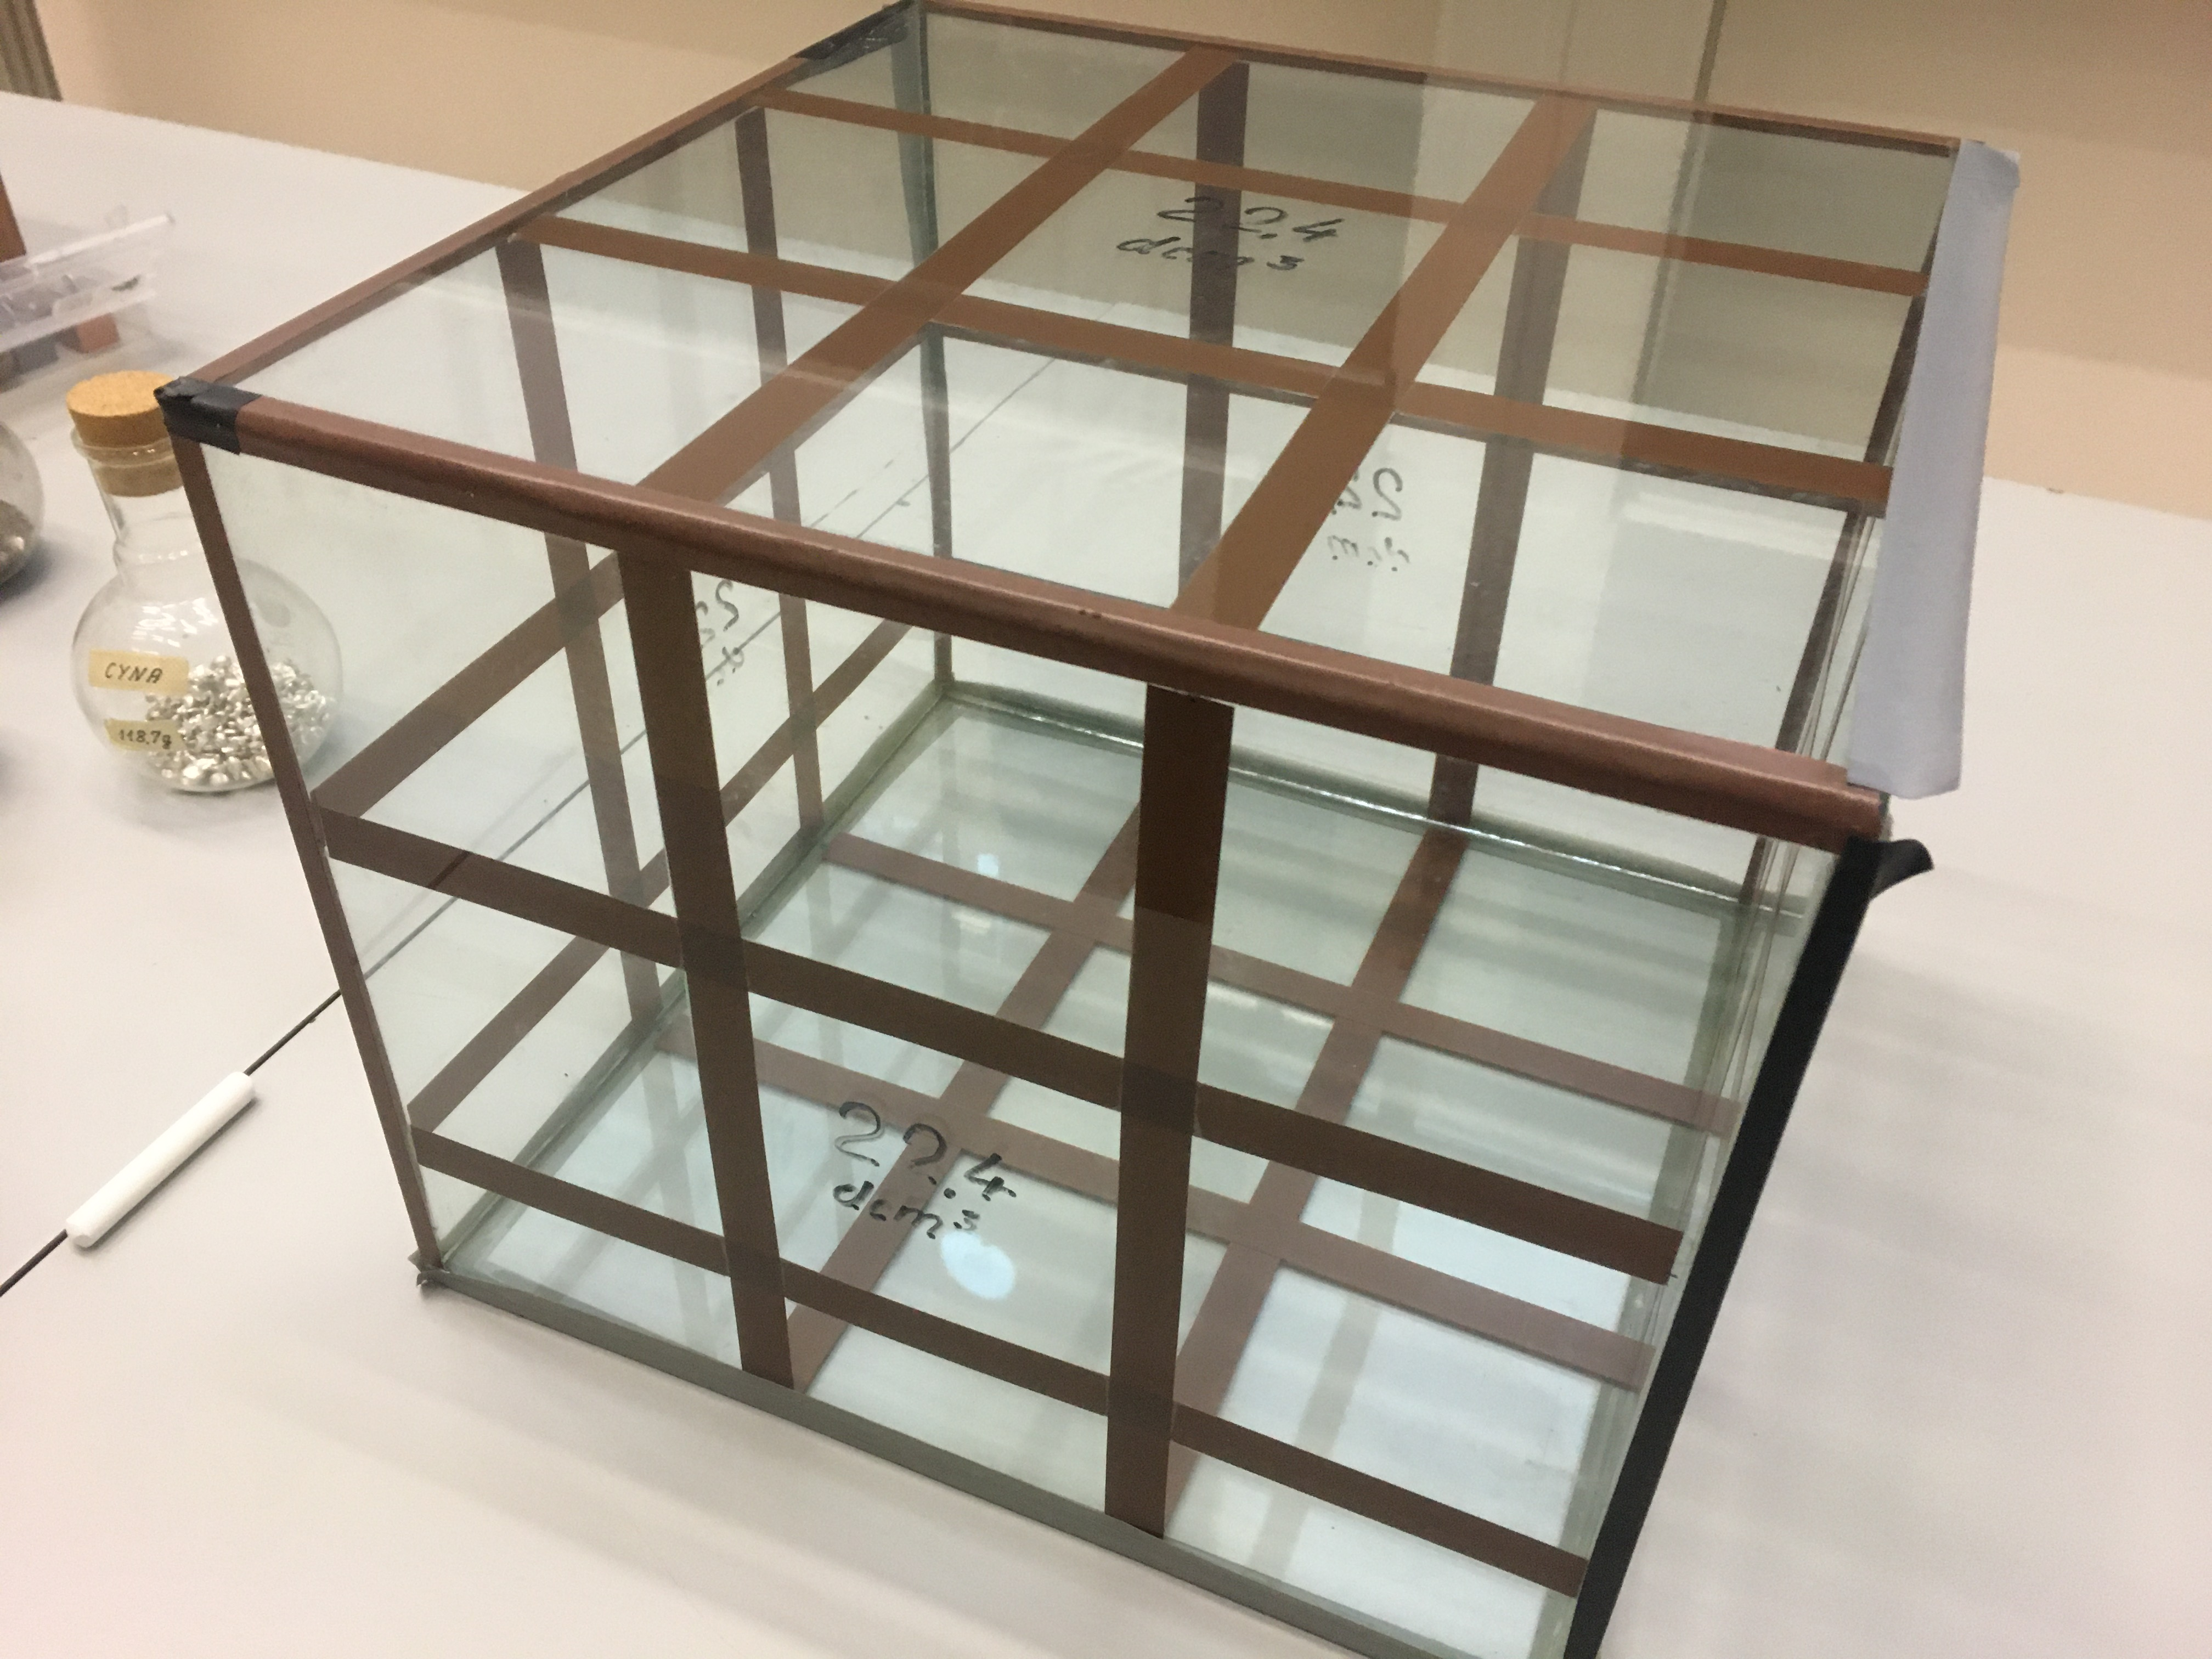
\includegraphics[width=0.5\linewidth]{Wyk_2_Rys_3.JPG}
    \caption{Jeden mol powietrza}
    \label{fig:lec_2:mol_pow}
\end{figure}

\begin{figure}[!ht]
    \centering
    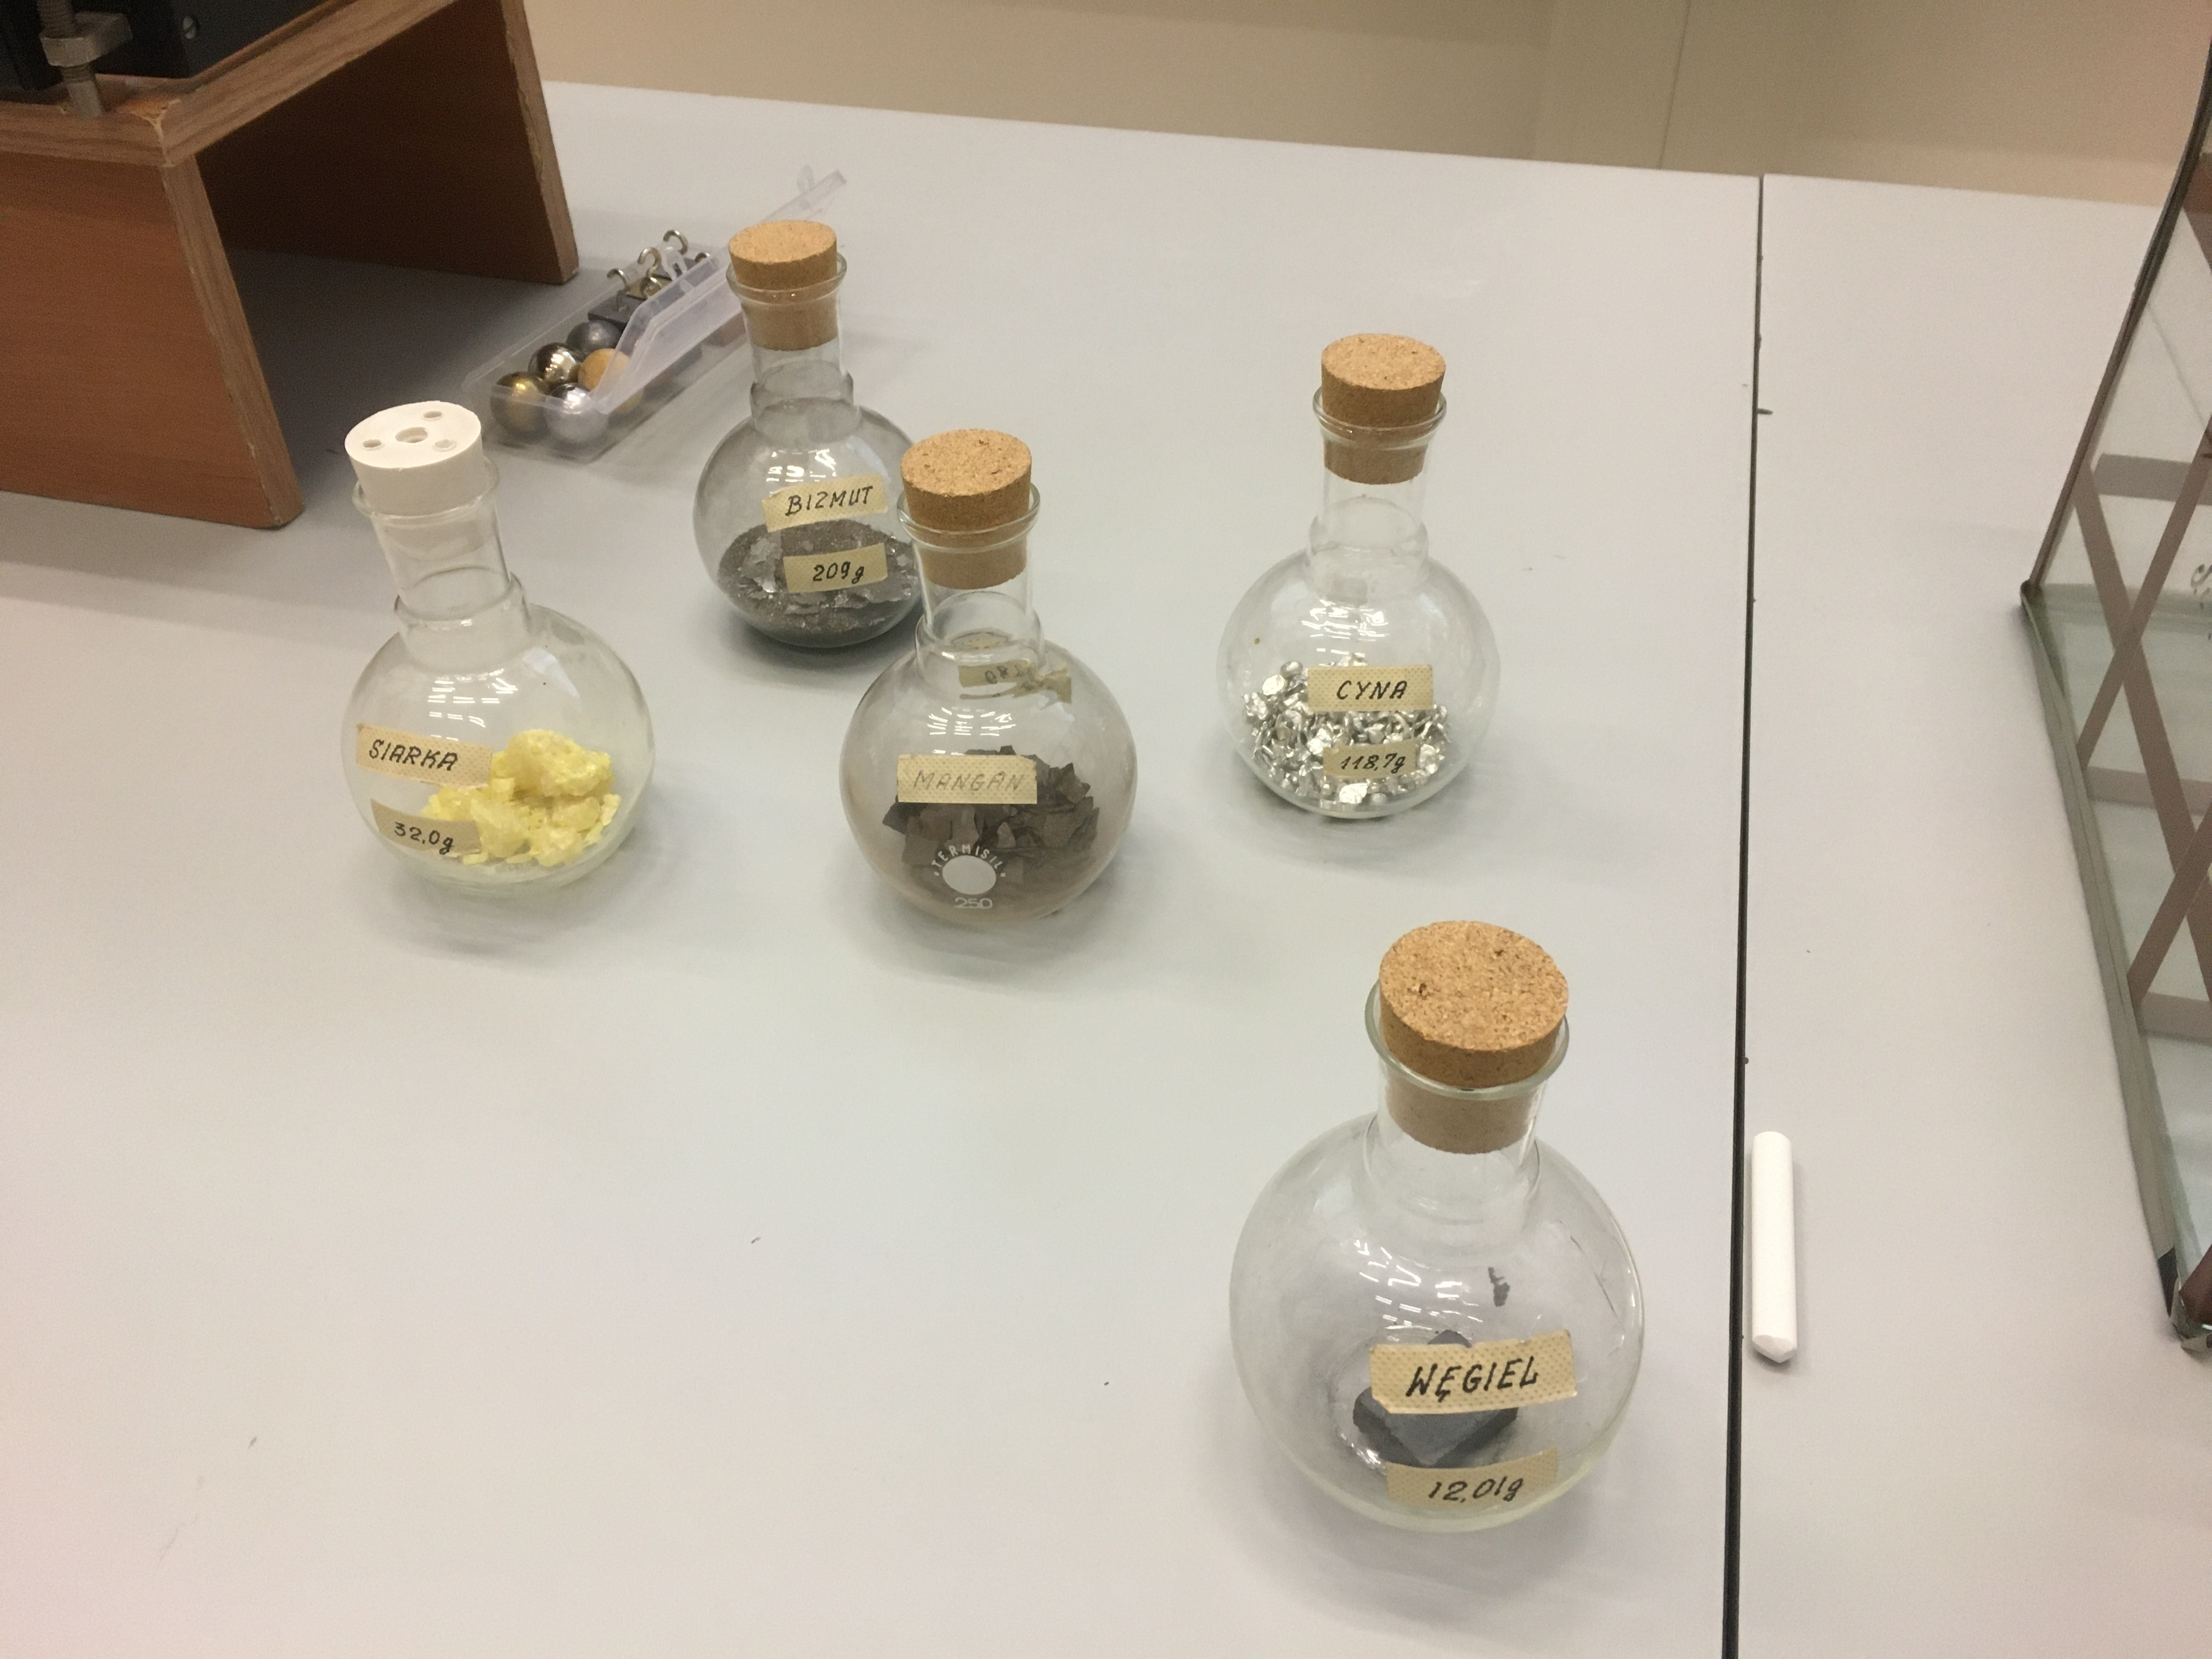
\includegraphics[width=0.8\linewidth]{Wyk_2_Rys_4.JPG}
    \caption{Jeden mol innych rzeczy}s
    \label{fig:lec_2:mole_demo}
\end{figure}

\begin{figure}[!ht]
    \centering
    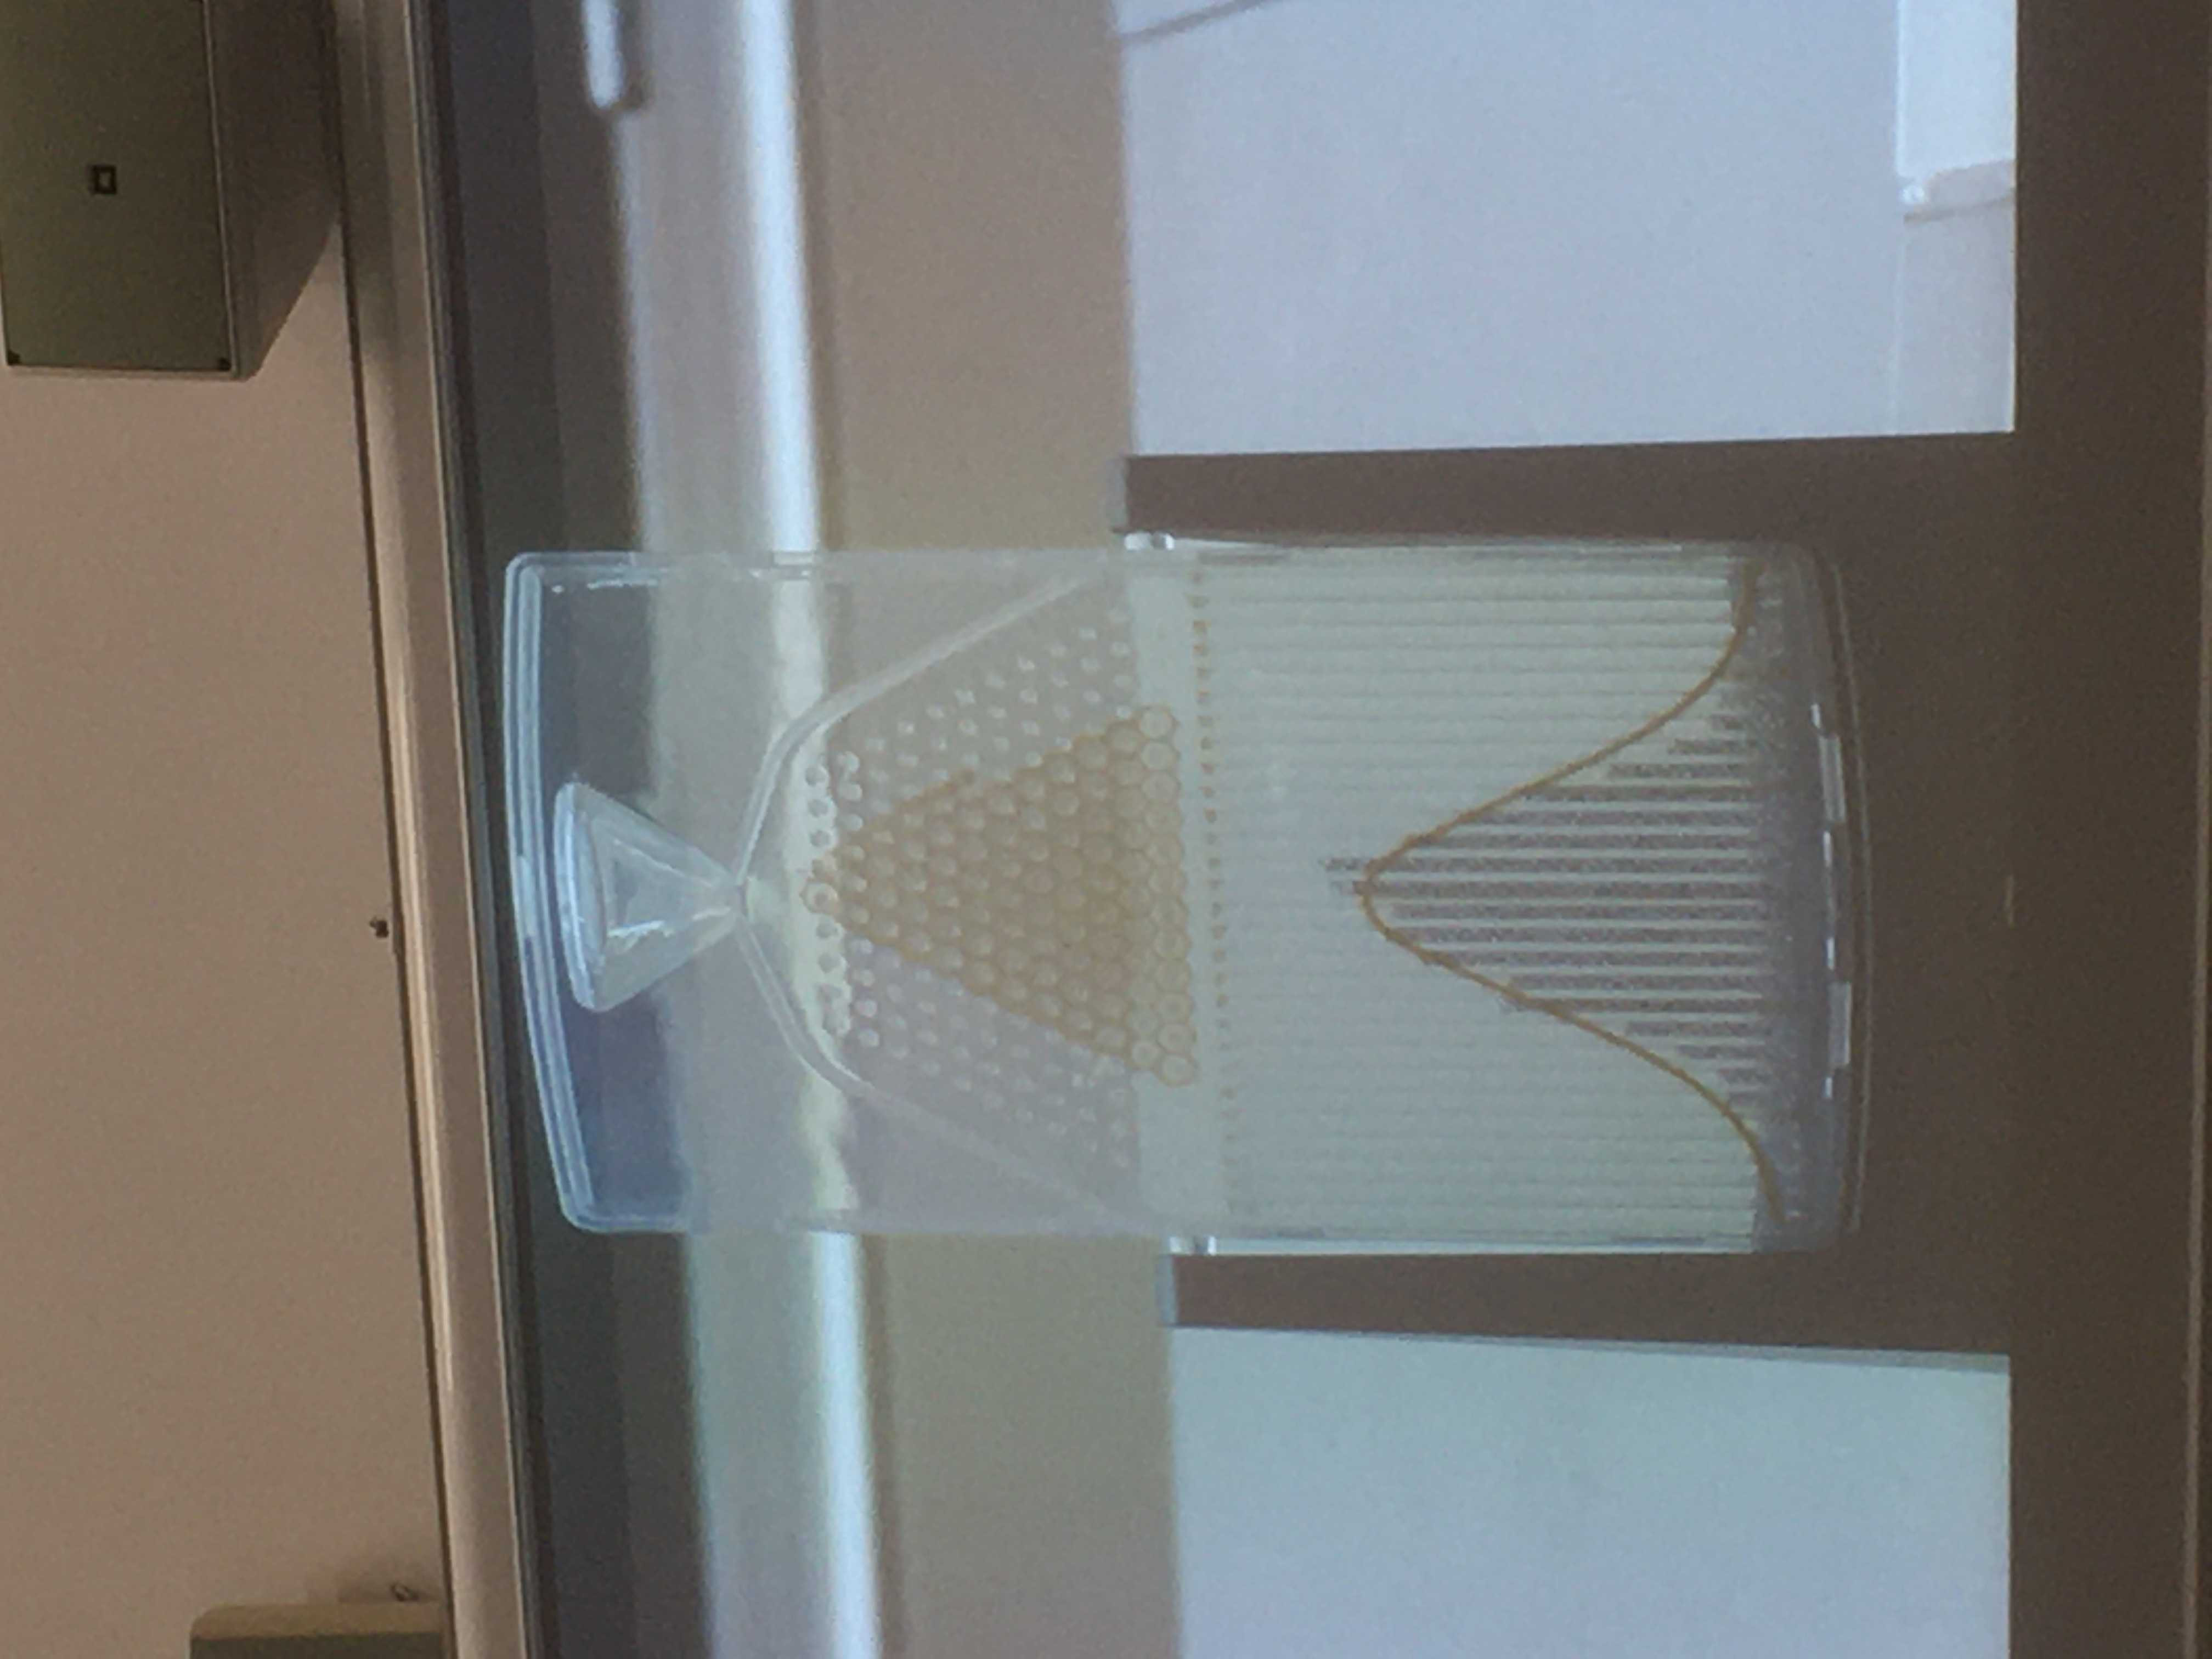
\includegraphics[width=0.8\linewidth, angle=270]{Wyk_2_Rys_5.JPG}
    \caption{Przykładowy \subind{Rozkład Gaussa}{Rozkład!Gaussa} uzyskany ze spadających kulek}
    \label{fig:lec_2:gauss}
\end{figure}

Teaser na przyszłość, dyfuzja z dodatkowym członem od pola siły.
\begin{equation}
    \pdv{P}{t} = D \pdv[2]{P}{x} - \pdv{F}{\gamma}P
    \label{eq:lec_2:dyfuzja_pelna}
\end{equation}

\FloatBarrier

\section{Wracamy do Modelu Erhnferstów}

\begin{align}
    P(n, t+1) = \frac{n+1}{N} P(n+1, t)+ (1 - \frac{n-1}{N}) P(n-1, t) \label{eq:lec_2:Psy_1}\\
    P(0, t+1) = \frac1N P(1, t)\label{eq:lec_2:Psy_2}\\
    P(N, t+1) = (1 - \frac{N - 1}{N}) P( N-1, t)\label{eq:lec_2:Psy_3}
\end{align}
Szukamy rozwiązania niezależnego od czasu - $p^{eq}(n)$. Z równania \ref{eq:lec_2:Psy_2} wynika:
\begin{align*}
    p^{eq}(0) &= a\qc p^{eq}(1) = Na\qc p^{eq}(n) = \mqty(N \\ n)a\\
    &\qq{\color{purple} Udowodnijmy przez indukcję:}\\
    &\begin{cases}
        p^{eq}(n-1) = a \mqty(N \\ n-1)\\
        p^{eq}(n) = a \mqty(N \\n)
    \end{cases}\\
    &\qq{\color{purple} Teraz biorąc równanie \ref{eq:lec_2:Psy_1} wyżej:}\\
    p^{eq}(n+1) \frac{n+1}{N} &= a \qty[\mqty(N \\ n) \mqty(N \\ n-1) \frac{N - n +1}{N}]\\ \\ \hline \hline
    &\qq{\color{purple}Pamiętając o tożsamości:}\\
    \mqty(N \\n) &= \mqty(N-1 \\ n) + \mqty(N-1 \\ n-1)\qq{dostajemy:}\\ \hline \hline \\
    p^{eq}(n+1) &= a \frac{N}{n +1}\qty[\qty{\mqty(N-1\\n) + \mqty(N-1 \\ n-1)} - \qty{\mqty(N-1 \\ n-1) + \mqty(N -1 \\ n-2)} \cdot \frac{N - n + 1}{N}]\\
    p^{eq}(n+1) &= a \frac{N}{n +1} \qty[\frac{(N-1)! N }{n! (N-1-n)! (n+1)} + \frac{(N-1)!}{(n-2)!(N-n)!(n+1)} - \frac{(N-1!)}{(n-2)!(N-n)! (n+1)}]\\
    p^{eq}(n+1) &= a\mqty(N \\ n+1)\\
    \implies& p^{eq}(n) = a \mqty(N \\n)
\end{align*}

\end{lecture}

% ---------------------------------------------------------------------
% Wykład 07.03.2022

\begin{lecture}{Definicja stanu, Entropia}

\begin{figure}[!ht]
    \centering
    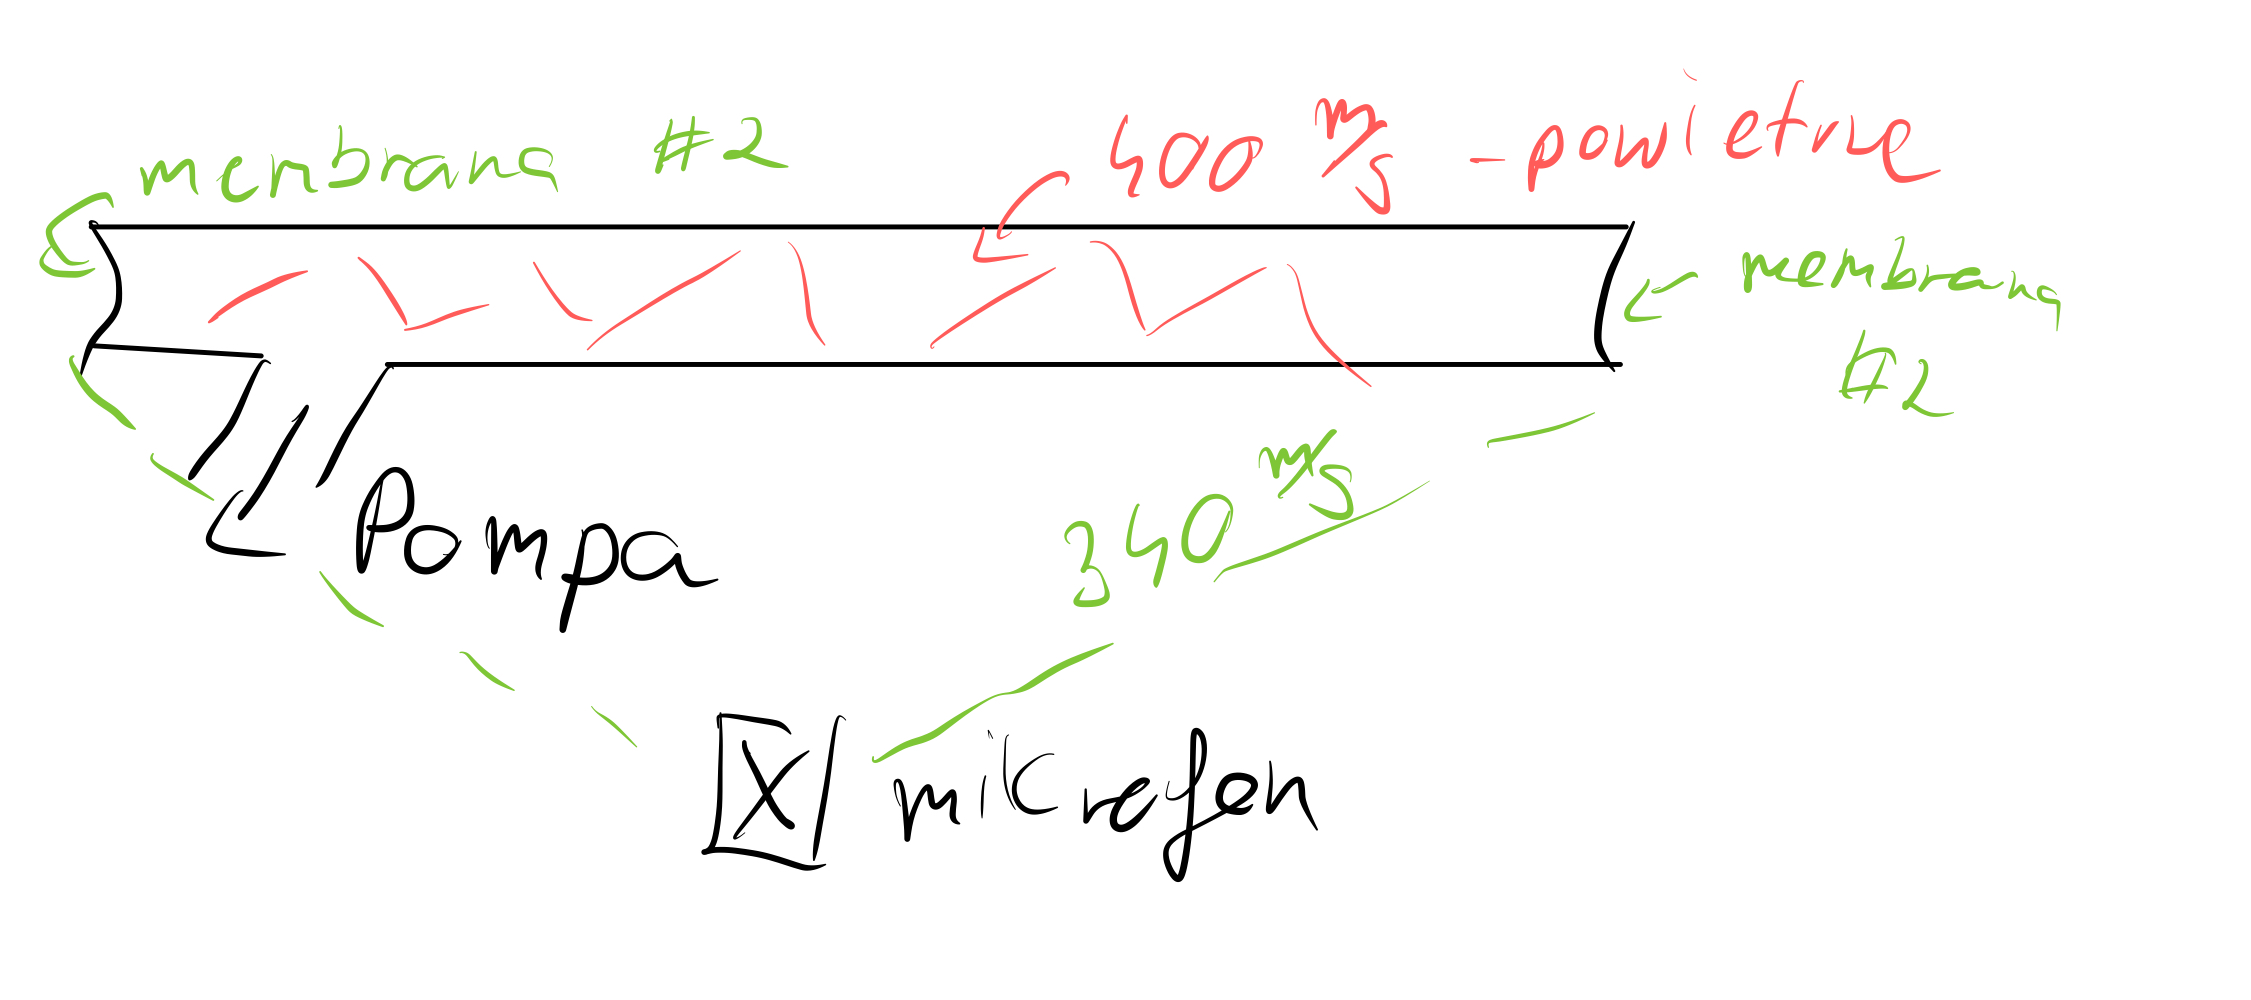
\includegraphics[width=0.8\linewidth, angle=0]{Wyk_3_Rys_1.jpeg}
    \caption{Doświadczenie pokazujące jaka jest prędkość cząsteczek powietrza w temperaturze pokojowej, tj. 400 m/s.}
    \label{fig:lec_3:v_pow}
\end{figure}

Powrót do 2 psów:
Na ostatnim wykładzie dostaliśmy równanie na równowagę. Wracamy do tego i idziemy dalej:

\[ p^{eq}(n) = a \mqty(N \\n) \]

Gdzie stała $a$ jest równa:
\begin{align*}
    &\sum_0^N a \mqty(N \\ n) = 1\\
    \hline \hline \\
    &\qq{pamiętając o tym, że:}\\
    (a+b)^N &= \sum_0^N \mqty(N \\ n) + a^n + b^n \qq{co po wstawieniu}  a = b =1\\
    \hline \hline \\
    2^N &= \sum_0^N \mqty(N \\ n) \implies a = \frac{1}{2^N}
\end{align*}



Możemy sobie to rozumieć jako fakt, że $p^{eq}$ odpowiada przyjęciu, że wszystkie możliwości są równo prawdopodobne.\\

Inaczej jeszcze patrząc na to; Wyobraźmy sobie, że każda pchła jest rozróżnialna i może być albo na Azorze albo na Burku. Wtedy takich możliwości jest $2^N$ i spośród nich $\mqty(N \\ n)$ z nich jest na Azorze.

\begin{emph_box}{Definicje stanów}
\ind{Mikrostan} - Informacja o położeniu każdej ze pcheł\\
\ind{Makrostan} - Informacja ile jest pcheł na Azorze
\end{emph_box}

Jednemu makrostanowi\footnote{$n$ pcheł na Azorze} będzie odpowiadać wiele mikrostanów\footnote{Dokładniej $\mqty(N\\n)$}. W szczególności:
\begin{itemize}
    \item Makrostanowi "wszystkie pchły na Azorze" odpowiada 1 mikrostan
    \item Makrostanowi $50\% - 50\%$ odpowiada $\mqty(N \\ N/2)$ mikrostanów,\footnote{Z tym, że $\mqty(N \\ N/2) \approx \frac{N!}{(N/2)!(N/2)!}\approx \frac{N^N}{(N/2)^{N/s} (N/2)^{N/2}} = 2^N$} czyli prawie wszystkie z dokładnością do $\sim N$.
\end{itemize}

Teraz wyobraźmy sobie, że układ osiąga stan równowagi. Wyprowadzimy sobie tutaj \subind{warunek równowagi szczegółowej}{warunek równowagi!szczegółowej}:
\begin{align*}
    p^{eq}(n) p(n\to n+1) &= p^{eq}(n+1)p(n+1 \to n)\\
    (1 - \frac{n}{N}) &= \frac{N-n}{N}\\
    p^{eq}(n+1) &= \frac{N-n}{n+1} \frac{N - (n-1)}{n}\\
    p^{eq}(n+1) &= \frac{(N-n) \dots N}{(n+1) n (n-1) \dots 1} p^{eq}(0)\footnotemark\\
    p^{eq}(n+1) &= \frac{N!}{(N-n-1)!(n+1)!}a \\
    p^{eq}(n+1) &= \mqty(N \\ n+1) a\\
    p^{eq}(n) &= \mqty(N \\ n) a
\end{align*}
\footnotetext{$=a$}



Teraz sprawdźmy, czy jesteśmy w stanie policzyć średnią liczbę pcheł na Azorze w funkcji czasu $\to \ev{n(t)}$, tj. ile średnio zmieni się $n$ przy jednym skoku pchły?

\[
    \begin{cases}
    p = \frac{N-n}{N} \qc "+1"\\
    p = \frac{n}{N} \qc "-1"
    \end{cases}
\]
Czyli zbadamy sobie zależność:
\[
    \ev{n(t+1)} - \ev{n(t)} = 1 - \frac{2 \ev{n(t)}}{N}
\]

\begin{align*}
    \ev{n(t+1)} &= 1 - \frac{2 \ev{n}}{N} + \ev{n} \qc n=\frac{N}{2} + m\\
    \ev{n(t+1)} &= \ev{n(t)}(1 - \frac{2}{N}) + 1\\
    \ev{m(t+1)} + \frac{N}{2} &= \ev{(\frac{N}{2} + m)(1 - \frac{2}{N})} + 1\\
    \ev{m(t+1)} &= (1 - \frac{2}{N}) m(t) = (1 - \frac{2}{N})^2 m(t-1)\\
    \ev{m(t)} &= (1 - \frac{2}{N})^t \frac{N}{2}
\end{align*}
Gdzie bierzemy:
\begin{itemize}
    \item $t$ - liczba kroków
    \item $\tau$ - czas między skokami
    \item $T = t \tau$ - czas
    \item $\frac{1}{N \tau} = \gamma = const.$ - ułamek pcheł, który przeskakuje w ciągu jednostki czasu.
\end{itemize}

I teraz przejdziemy do granicy $N \to \infty \qc \tau \to 0$:
\[
    \ev{f(t)} = \ev{\frac{2m(t)}{N}}\footnotemark = \qty(\qty(1 - \frac{2}{N})^{-\frac{2}{N}})^{-\frac{2 T}{N \tau}}
\]
\footnotetext{Względna nadwyżka}

Co daje nam zanik wykładniczy:
\[
    \ev{f(t)} = e^{- 2 T \gamma}
\]
\end{lecture}

\ind{Mierzenie informacji}

\begin{figure}[!ht]
    \centering
    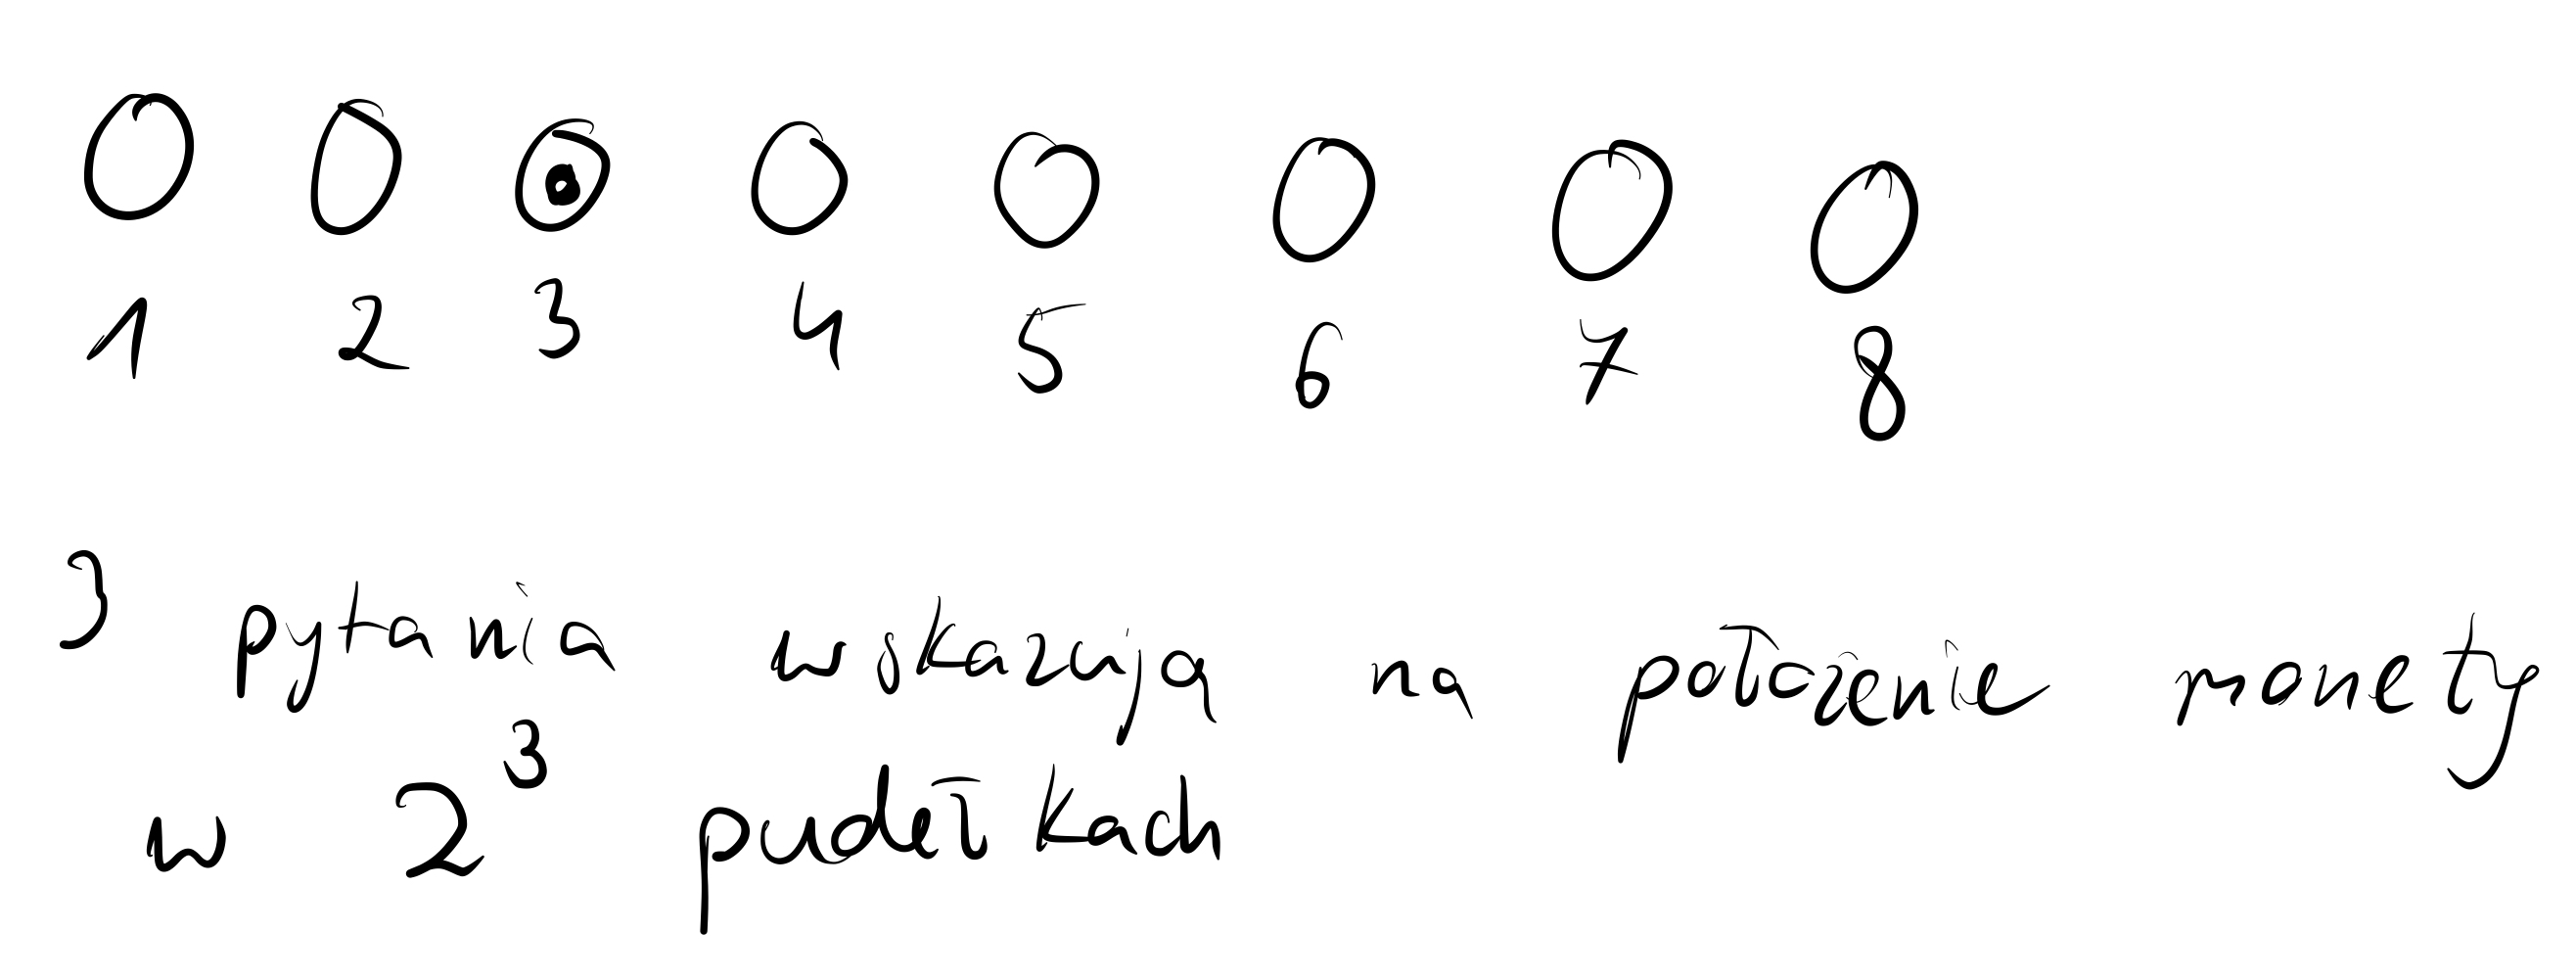
\includegraphics[width=0.8\linewidth, angle=0]{Wyk_3_Rys_2.jpeg}
    \caption{Osiem identycznych pudełek.}
    \label{fig:lec_3:inf_1}
\end{figure}

Jak widać na Rysunku \ref{fig:lec_3:inf_1}, nasza Informacja to będzie:
\begin{align*}
    N = 2^n\\
    \log N = n \log 2 \\
    n = \frac{\log N}{\log 2} = k \log N
\end{align*}

\begin{figure}[!ht]
    \centering
    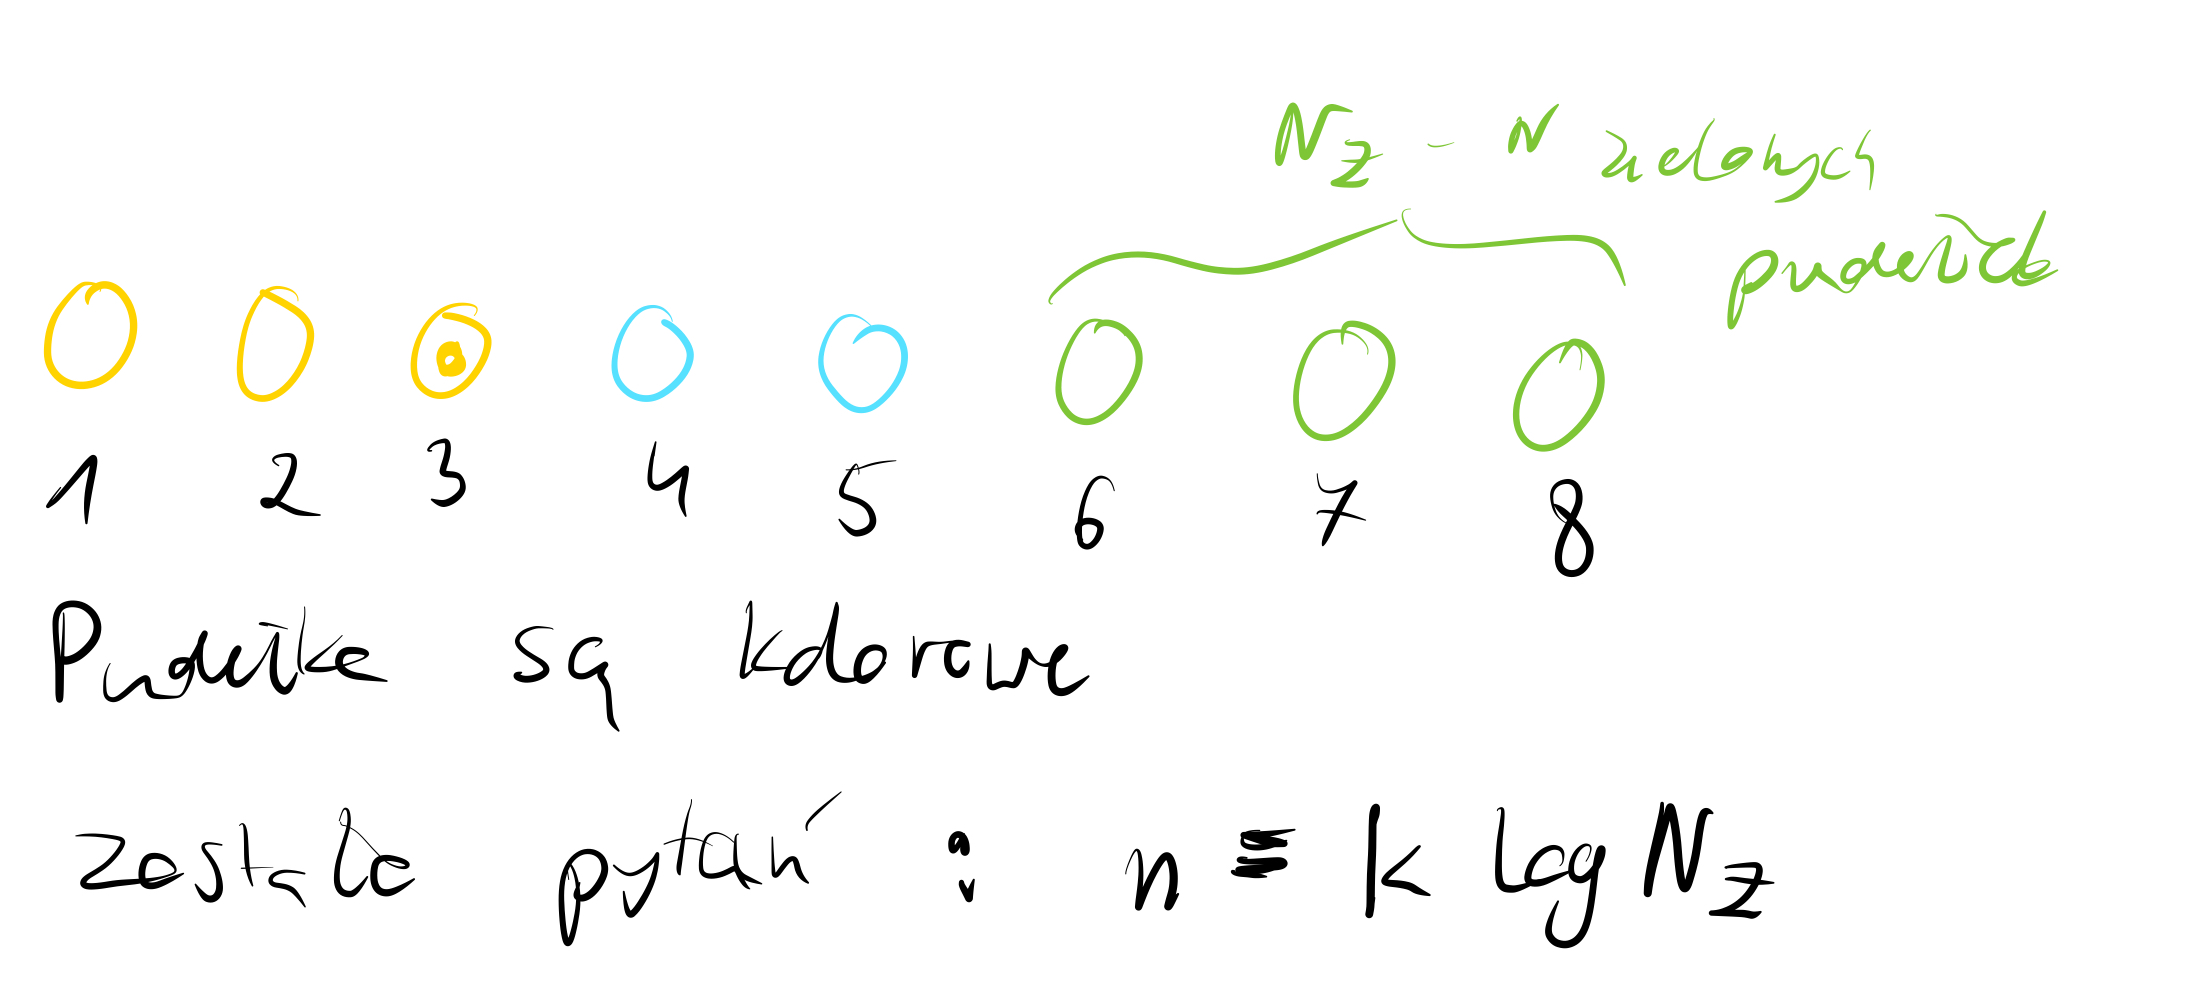
\includegraphics[width=0.8\linewidth, angle=0]{Wyk_3_Rys_3.jpeg}
    \caption{Osiem kolorowych pudełek}
    \label{fig:lec_3:inf_2}
\end{figure}

Teraz jak widzimy na Rysunku \ref{fig:lec_3:inf_2}, gdy pudełka mają dodatkową cechę rozróżniającą je, to zdobywajac ją możemy zawęzić sobie pole wyboru. Teraz wyobrażamy sobie, że mamy szpiega, który nam ma powiedzie w pudełku jakiego kolowu jest moneta w tym układzie.\\
Bez kolorów mieliśmy do zadania $n = k \log N$ pytań, zaś wraz z kolorami mamy $n = k \log N_z$ pytań, czyli to jak dużo informacji dostarczył nam szpieg (ilu pytań nam oszczędził) wyrazi się jako:
\(
    I_z = k \log N - k \log N_z = -k \log(\frac{N_z}{N})
\)
Gdzie $\frac{N_z}{N}$ jest jednocześnie procentem pudełek koloru który nam wskazał szpieg (tu: zielonych), jak i prawdopodobieństwem, że moneta jest w pudełku tego koloru. Ogólnie daje nam to:
\[
    I_i = -k \log p_i
\]

Teraz średnią miarę tego naszego 'zdziwienia ilością informacji od szpiega' oznaczymy wzorem:
\[
    I = \sum_i -k p_i \log p_i
\]
Jest to \ind{Informacja Shannona} Inna nazwa to \subind{Entropia Informacyjna Shannona}{Entropia!Informacyjna Shannona}.

Wnioski:

\begin{enumerate}
    \item Dla rozkładu równowagowego (wszystkie zdarzenia równoprawdopodobne) $p_i = \frac{1}{N}$, $N$ - liczba zdarzeń.\\
    $I = \sum_i -k \frac{1}{N} \log \frac{1}{N} = k \log N$
    \item Dla rozkładu maksymalnie nierównowagowego $p_1 = 1 , p_2 = \dots = 0$. Wtedy $I = 0$.
    \item Można pokazać, że rozkład równowagowy maksymalizuje Entropię. Jest to tzw twierdzenie Jensena dla fukncji wklęsłych. \com{Zdjęcie wklej}
\end{enumerate}
% ------------------------------------------------------------------------
% 10.03.2022

\begin{lecture}{Entropia Gibbsa i Boltzmanna}

\emph{Wzór J.W.Gibbsa}
\[
    S = - k \sum_i p_i\footnote{Prawdopodobieńśtwo wystąpienia mikrostanu} \log p_i
\]

\emph{Joseph Willard Gibbs} (1893 - 1903) \textit{Elementary Principles in Satistical Mechanics (1907)}

\emph{Wzór Boltzmanna}
\[
    S = k \log W\footnote{Liczba mikrostanów}
\]

\section{Psy Ehrenfersta}

\subsection{Wzrost Entropii}

\begin{itemize}
    \item $G_m$ - liczba mikrostanów odpowiadającuch makrostanom $m$, $G_m = \mqty(N \\ m)$
    \item $P_m(t)$ - prawdopodobieństwo makrostanu ($m$ pcheł na Azorze)
    \item $p_i(t)$ - prawdopodobieństwo mikrostanu, $p_i (t) = \frac{P_m(t)}{G_m(t)}$\footnote{Wszystkie mikrostany odpowiadające makrostanom $m(i)$ są równoprawdopodobne.}
\end{itemize}

\begin{emph_box}{\ind{Entropia}}
\[
    S = - k \sum_{i=1}^{2^N} p_i \log p_i =\footnotemark - k \sum_m G_m \frac{P_m}{G_m} \log \frac{P_m}{G_m}
\]
\[
    S = \underbrace{- k \sum_m P_m \log P_m}_{\footnotemark} + \underbrace{\sum_m P_m \overbrace{(k \log G_m)}^{\footnotemark}}_{\footnotemark}
\]
Czyli finalnie wzór na \emph{\subind{Entropię Boltzmanna}{Entropia!Boltzmanna}}:
\begin{equation}
    S_B = k \log G_m
    \label{eq:lec_4:entropia_boltz}
\end{equation}
Oraz wzór na \emph{\subind{Entropię Gibbsa}{Entropia!Gibbsa}}
\begin{equation}
    S_G = - k \sum_i p_i\footnote{Prawdopodobieńśtwo wystąpienia mikrostanu} \log p_i
    \label{eq:app:entropia_gibbs}
\end{equation}
\end{emph_box}
\footnotetext{Wymierny stopień obsadzenai różnych makrostanów}
\footnotetext{Entropia Boltzmanna odpowiadająca makrostanom M}
\footnotetext{Średnia entropia Boltzmanna}
\footnotetext{Tu zmiana indeksu sumowania, na sumowanie po makrostanach a nie mikrostanach}

Teraz idziemy dalej, pokażemy, że Entropia wzrasta. Zdefiniujmy:\\
$\pi_m = \frac{P_m}{G_m}$ - prawdopodobieństwo wystąpienia mikrostanu odpowiadającego makrostanowi $m$. Czyli:\\
$P_m = \pi_m G_m \implies$
\[
    S = - \sum_m \pi_m G_m \log \pi_m
\]
Pokażemy, że:
\[
    \underbrace{- \sum \pi_m(t+1) G_m (t+1)}_{S(t+1)} \geq \underbrace{- \sum \pi_m (t) G_m \log \pi_m (t)}_{S(t)}
\]

Teraz skorzystamy z twierdzenia Jensena i Równania \subind{Master}{Równanie!Master}:\\
Funkcja $\phi(x) = x \log x$ jest wypukła $\implies$ 
\[
    \phi(\sum_i \alpha_i x_i) \leq \sum_i \alpha_i q(x_i)
\]
Równanie Master:
\begin{align*}
    P_m(t+1) &= \frac{m+1}{N} P_{m+1}(t) + (1 - \frac{m-1}{N} P_{m-1}(t))\\
    \pi_m (t+1) &= \frac{m+1}{N} \pi_{m+1} (t) \frac{G_{m+1}}{G_m} + \qty(1 - \frac{m-1}{N} \pi_{m-1} (t) \frac{G_{m-1}}{G_m})\\
    \pi_m (t+1) &= \underbrace{\frac{m}{N}}_{\alpha_1} \pi_{m-1}(t) + \underbrace{(1 - \frac{m}{N})}_{\alpha_2} \pi_{m+1}(t)\\
    \alpha_1 + \alpha_2 &= 1 \qc \varphi(x) = x \log x\\
    \varphi(\alpha_1 x_1 + \alpha_2  x_2) &\leq \alpha_1 q(x_1) + \alpha_2  q(x_2)\\
    \pi_m (t+1) \log \pi_m (t+1) &\leq \frac{m}{N} \pi_{m-1} (t) \log \pi_{m-1} (t) + (1 - \frac{m}{N}) \pi_{m+1} (t) \log \pi_{m+1} (t) 
\end{align*}
Teraz przemnóżmy przez $G_m$ i wysumujmy po $m$, daje nam to:
\[
    \underbrace{\sum_{m=0}^N \pi_m(t+1) G_m }_{-S_G(t+1)} \leq \underbrace{\sum_{m=0}^N G_m \frac{m}{N} \pi_{m-1} (t) \log \pi_{m-1} (t)}_{N1} + \underbrace{\sum_{m=0}^N G_m (1 - \frac{m}{N}) \pi_{m+1} (t) \log \pi_{m+1} (t)}_{N2}
\]

\[
    N1 = \sum_{n=0}^{N-1} \mqty(N-1 \\ n) \pi_n \log \pi_n \qc N2 = \sum_{n=0}^{N-1} \mqty(N-1 \\ n-1) \pi_n \log \pi_n
\]
Czyli:
\begin{align*}
    N1 + N2 &= \sum_{n=0}^{N-1} \pi_n \log \pi_n \qty(\mqty(N-1 \\ n) + \mqty(N-1 \\ n-1)) + \pi_N \log \pi_N + \pi_0 \log \pi_0\\
    &= \sum_{n=0}^{N} \mqty(N \\ n) \pi_n (t) \log \pi_n (t) = -S_G(t)\footnotemark
\end{align*}
\footnotetext{Entropia Gibbsa}
Czyli:
\begin{equation}
    S_G (t+1) \geq S_G (t)
    \label{eq:lec_4:wzrost_entropii}
\end{equation}
Czyli Entropia rośnie i osiąga maksimum w stanie równowagi <- \ind{Druga Zasada Termodynamiki}

A teraz co się dzieje w Entropią Boltzmanna? TL;DR -> Dla niej jest to tylko statystycznie, bo są fluktuacje które mogą być duże.
\\
\com{Przepisz ze zdjęcia}
\begin{figure}[!ht]
    \centering
    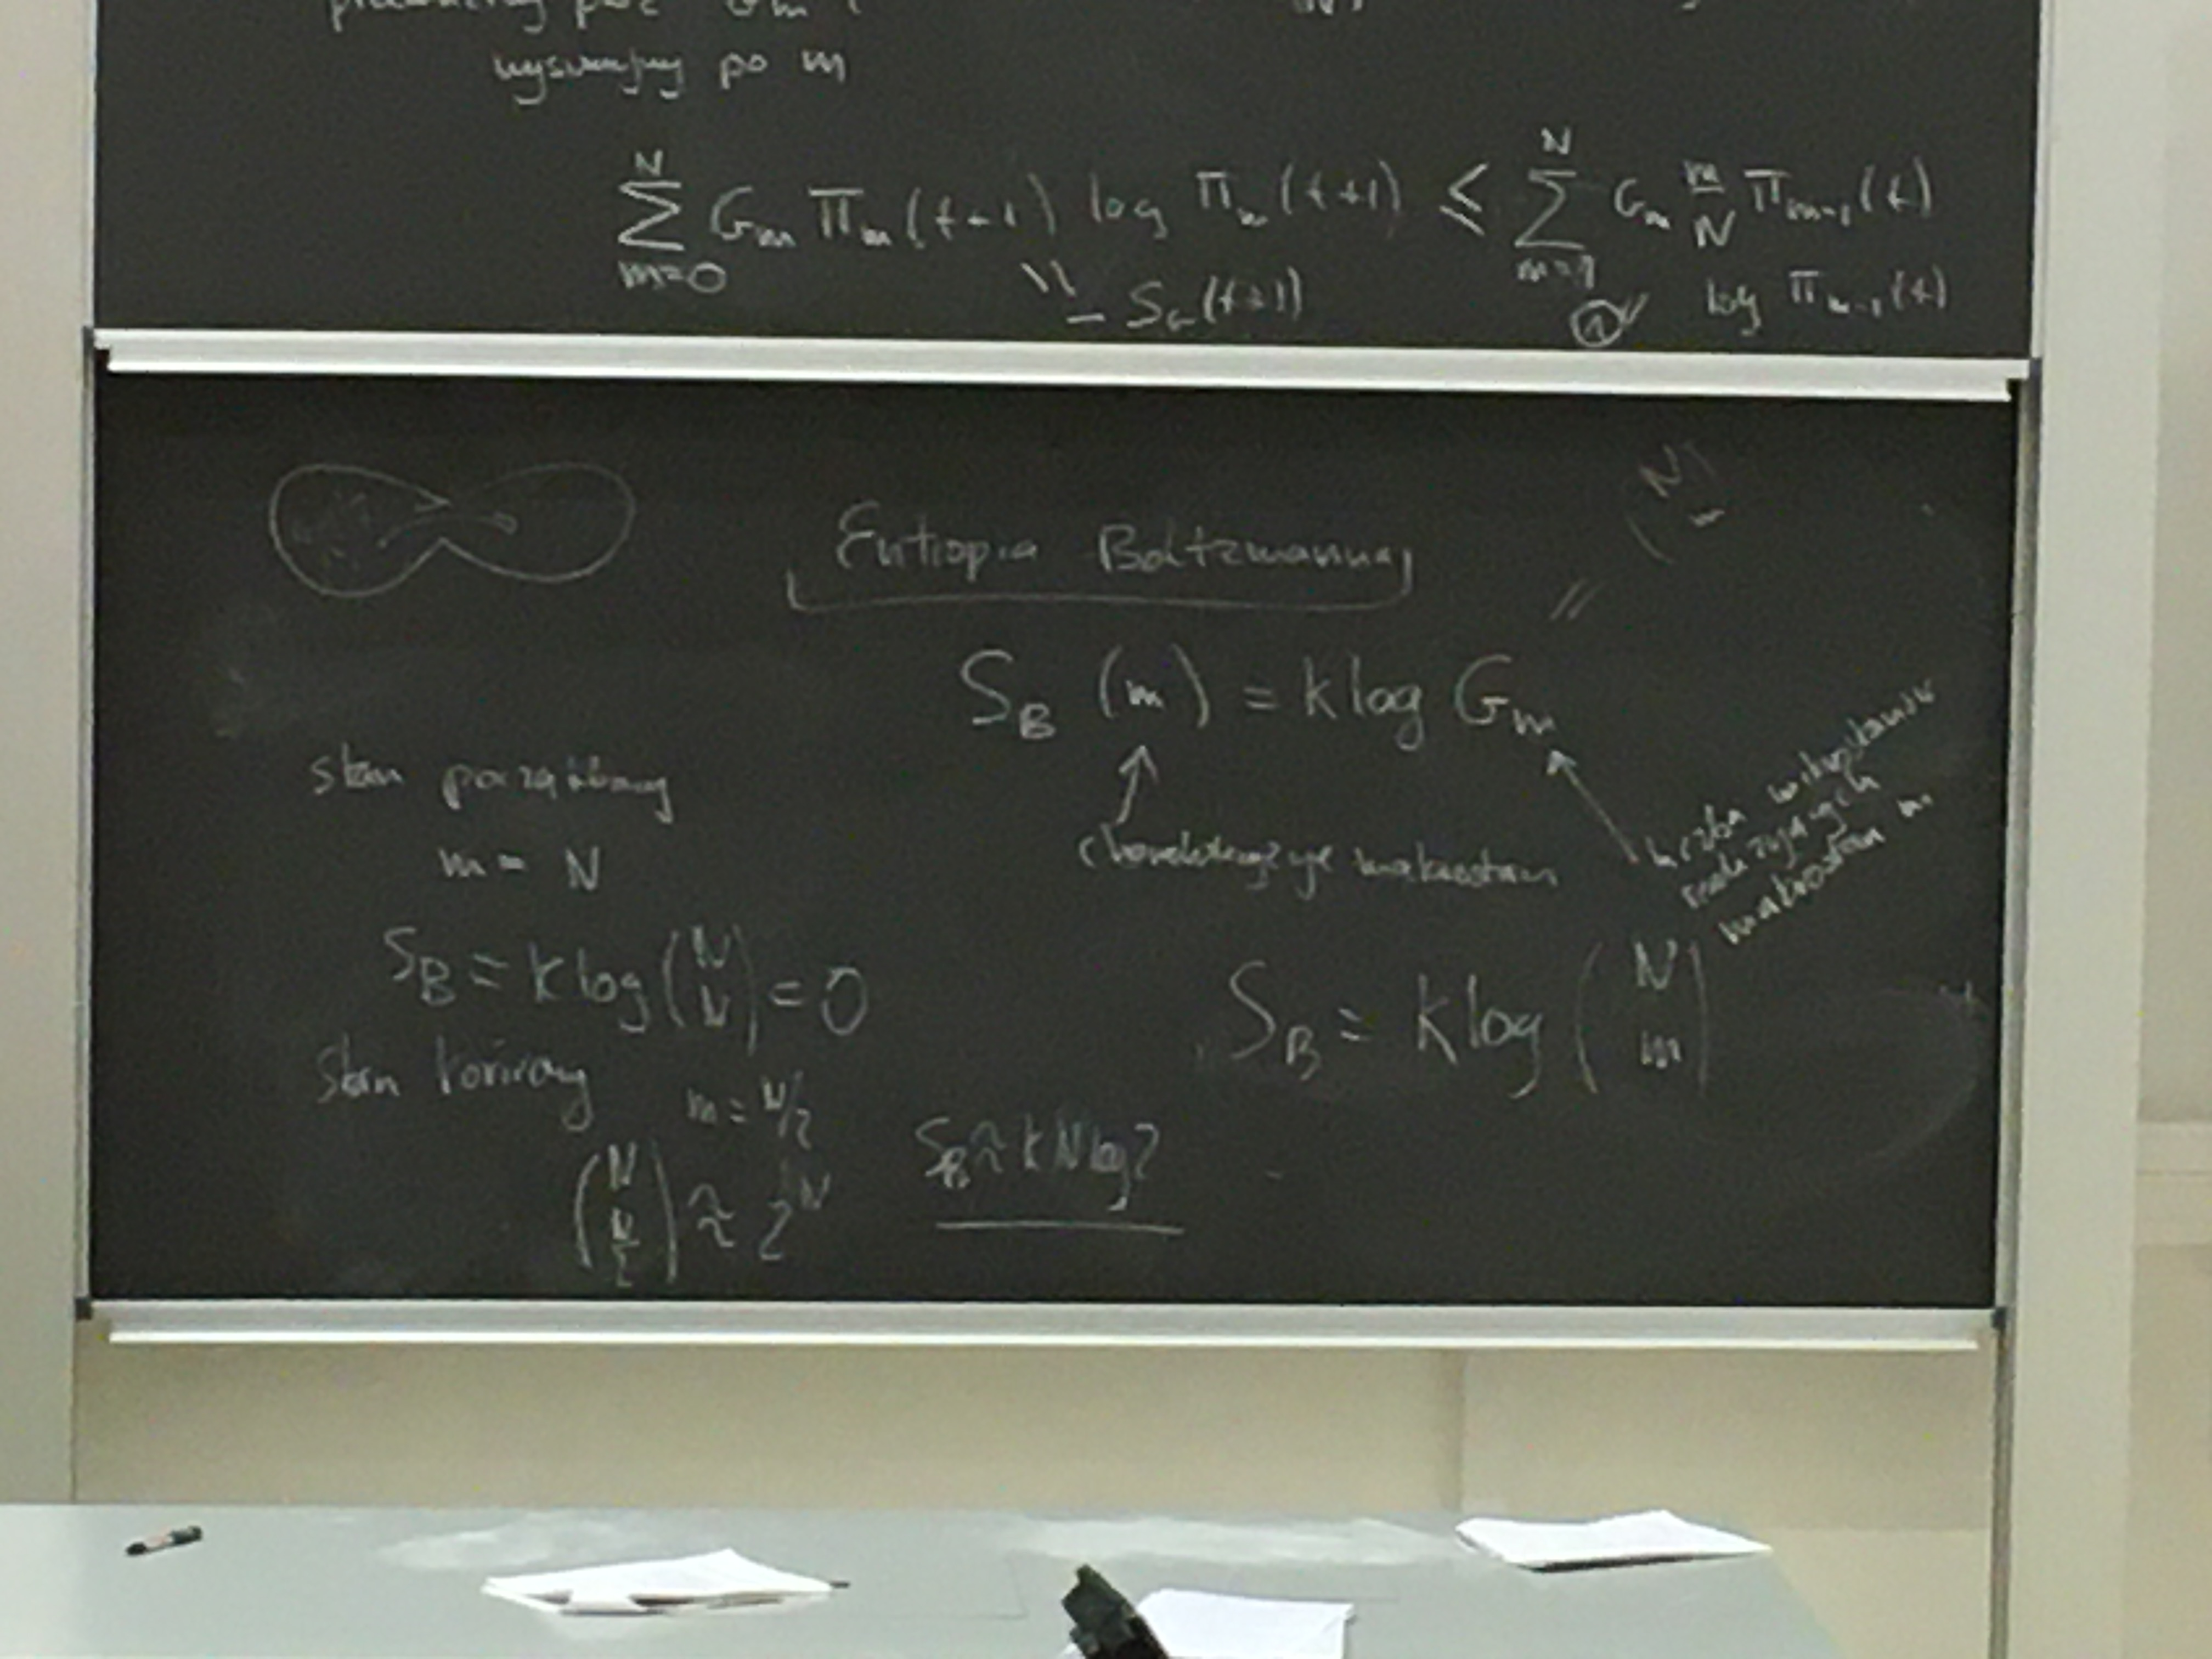
\includegraphics[width=0.8\linewidth, angle=0]{Wyk_4_Rys_1.JPG}
    \caption{\com{Przepisz to}}
    \label{fig:lec_4:cos_1}
\end{figure}

\begin{figure}[!ht]
    \centering
    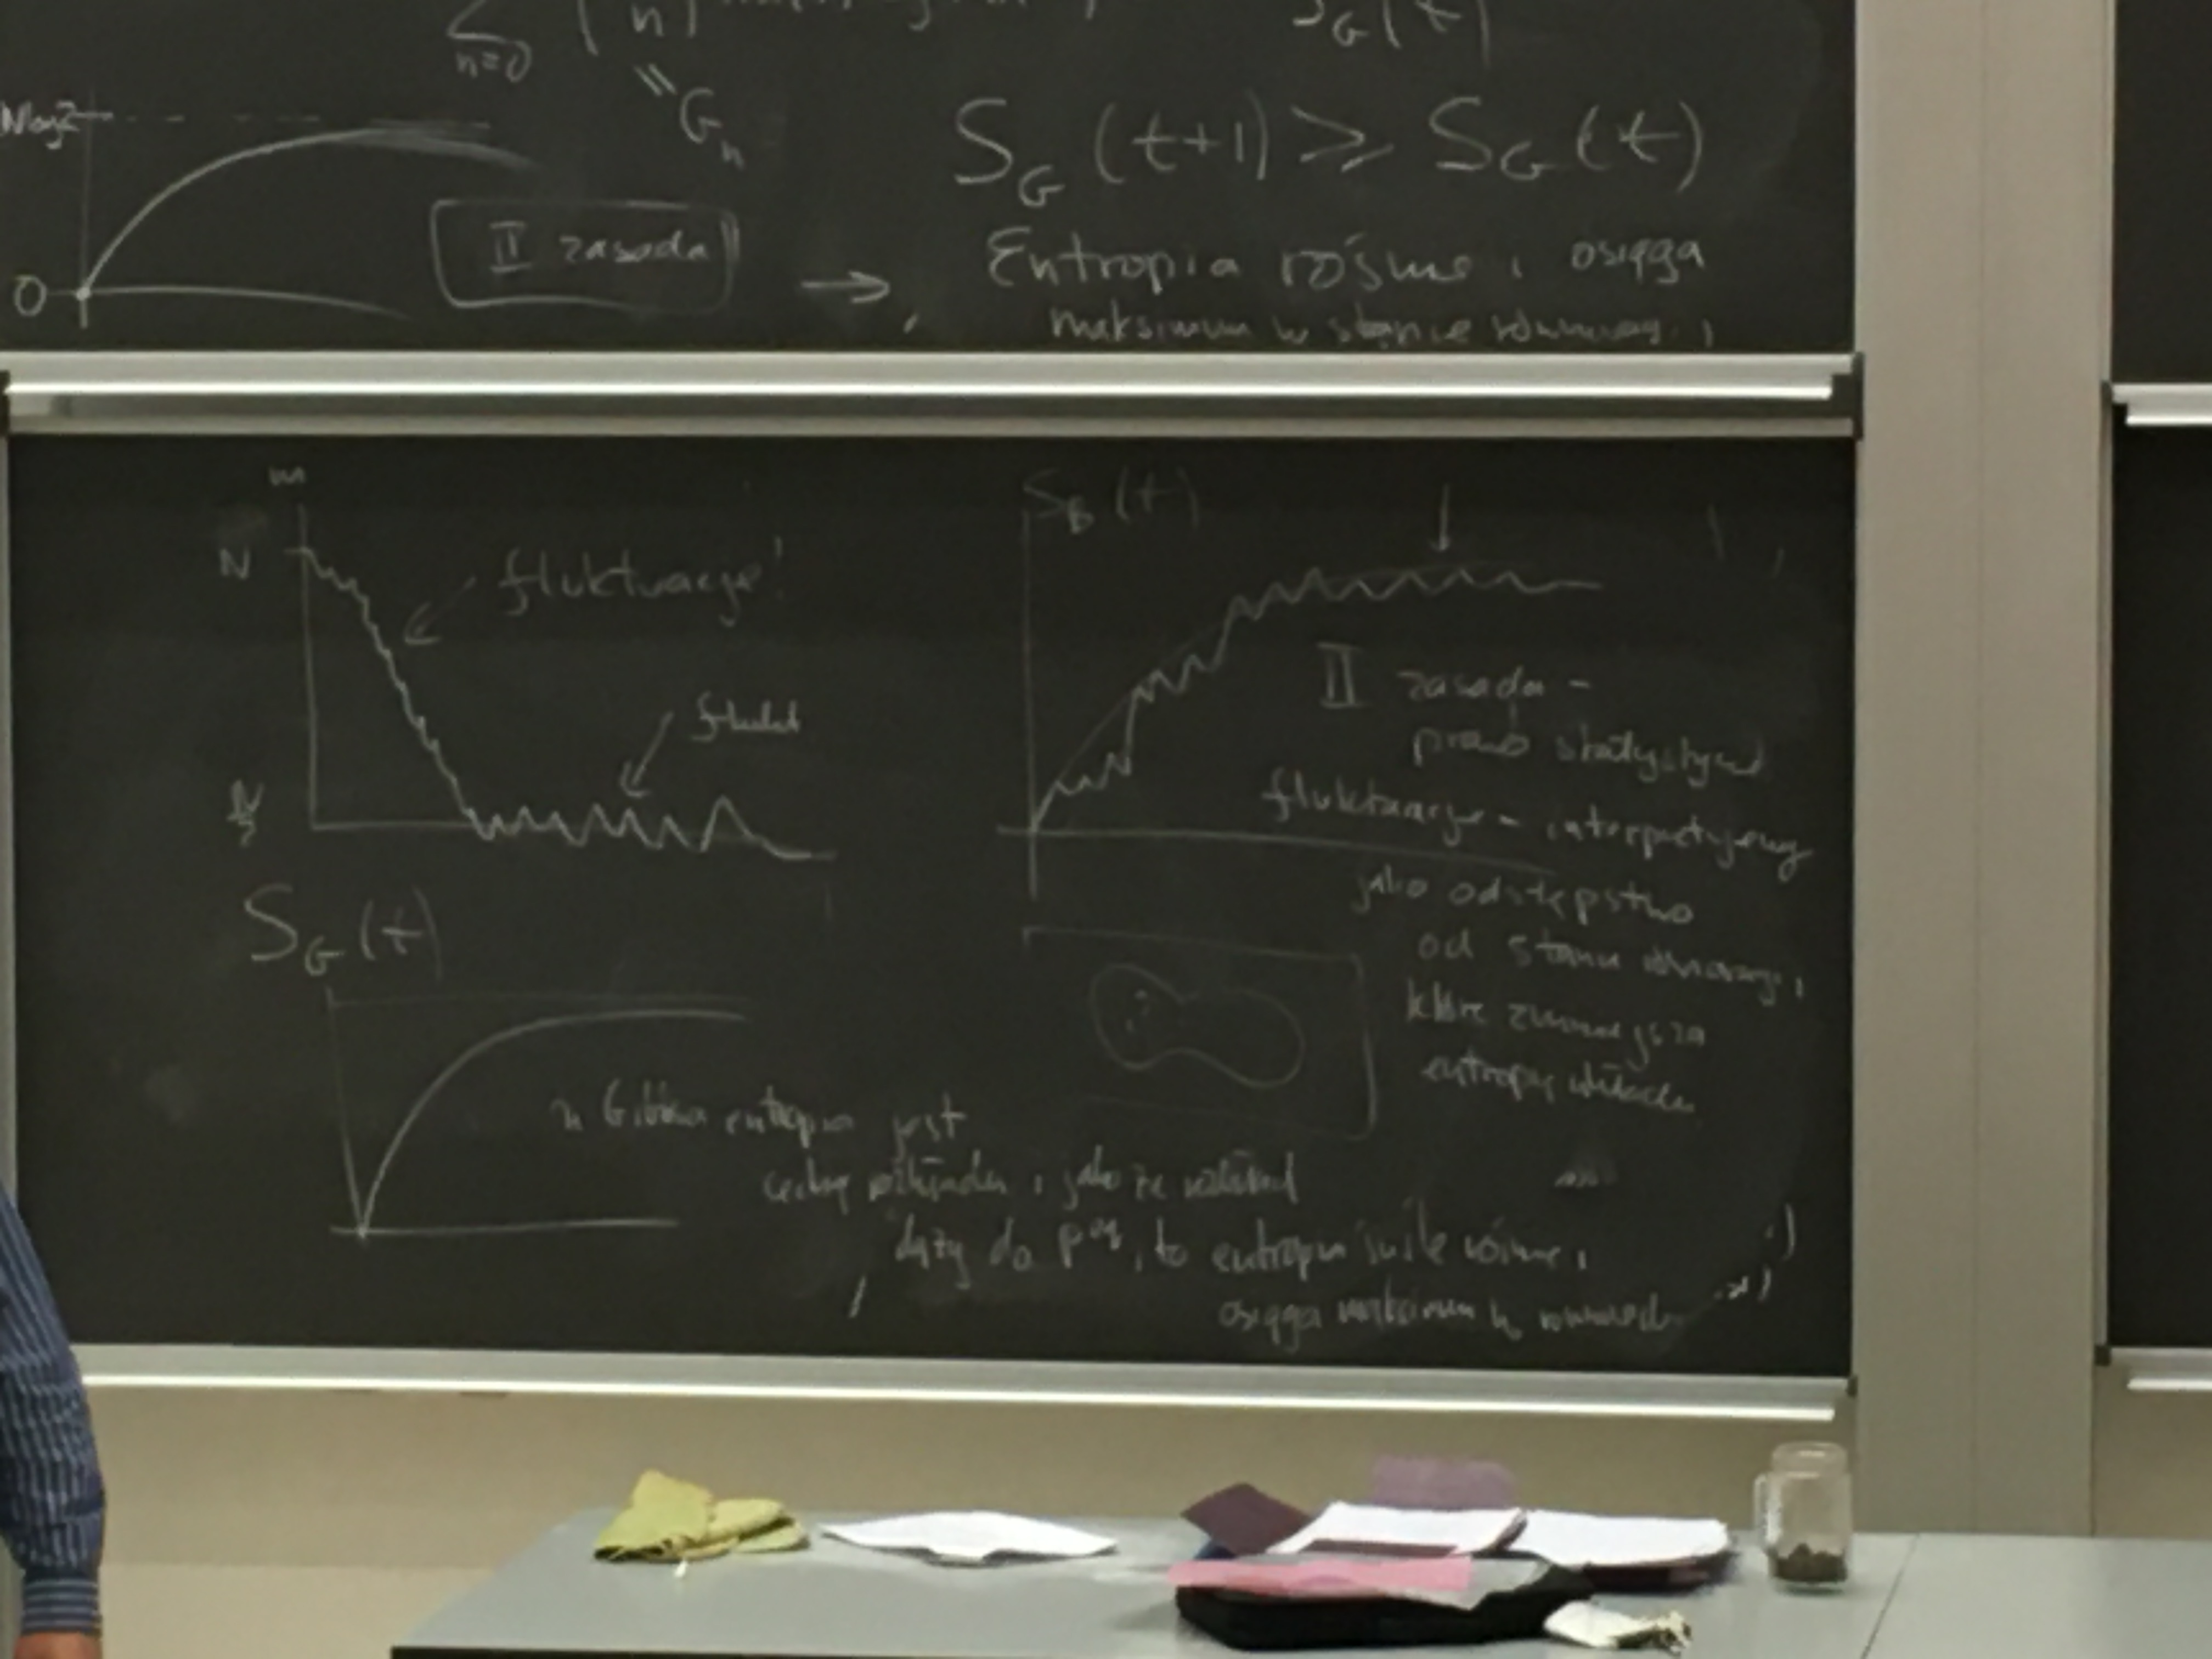
\includegraphics[width=0.8\linewidth, angle=0]{Wyk_4_Rys_2.JPG}
    \caption{\com{Przepisz to}}
    \label{fig:lec_4:cos_2}
\end{figure}

\FloatBarrier

Główne postulaty fizyki Statystycznej: (By Boltzmann)
\begin{itemize}
    \item W układzie makroskopowym procesy spontaniczne (dziejące się po usunięciu więzów)\\
    Przebiegają tak, ze liczba mikrostanów odpowiadajacych danemu makrostanowi rośnie\footnote{Z dokładnością do fluktuacji}
    \item Stanowi równowagi odpowiada makrostan, który realizuje największa liczba mikrostanów.
    \item Jeśli układ izolowany jest w stanie równowagi, to wszystkie stany można traktować jako równo prawdopodobne. <- postulat równych prawdopodobieństw \textit{a priori}
\end{itemize}

\end{lecture}

% ------------------------------------------------------------------------------------
% 14.03.2022

\begin{lecture}{Granica Termodynamiczna, Maksymalizacja Entropii}

\section{Przeniosło Time}

Psy Erhenferstów once again:\\
Niech liczba pcheł $N = 20000$\\
Prawdopodobieństwo liczby $n$ pcheł: $p(n) = \frac{1}{2^N} \qty(N \\ n)$
Side note: $N! = N^N e^{-N} \sqrt{a \pi N}$, Czas dojścia do stanu $\approx \frac{1}{p(n)}$
Czyli w szczególności wiedząc, że $p(0) = \frac{1}{2^N}$, $p(\frac{N}{2}) = \frac{1}{2^N} \mqty(N \\ \frac{N}{2})$:
\[
    T_0 = \frac{1}{p(0)} = 2^N = 2^20000 \approx (2^10)^2000 \approx (10^3)^2000 - \qq{absurdalnie duża liczba}
\]
Za to prawdopodobieńśtwo dojścia do stanu pół na pół:
\[
    p(N/2) = \frac{1}{2^N} \mqty(N \\ \frac{N}{2}) = \frac{1}{2^N} \frac{N!}{\qty(\frac{N}{2})!\qty(\frac{N}{2})!} \approx \frac{2}{\sqrt{2 \pi N}}
\]
Czyli czas dojścia:
\[
    T_{\frac{N}{2}} \approx \frac{1}{p(N/2)} = \frac{\sqrt{2 \pi} \sqrt{N}}{2} = 100 \sqrt{\pi} \approx 177\qq{s}
\]
Rozkład stanów prawdopoodobnych ma kształt bardzo cienkiego Gaussa, o szerokości $\sqrt{4 N}$

Side note: 1 Angstrem \AA$= 10^{-10}$

\section{Granica Termodynamiczna}
Weźmy:
\begin{itemize}
    \item Komórki o objętości $V_0 = 1$
    \item $V$ - komórek = liczba komórek = objętość w tej jednostce
\end{itemize}

Teraz wprowadźmy nowe pojęcie:

\begin{emph_box}{\ind{Granica Termodynamiczna}}
    Granica termodynamiczna, tj:
    \[
        N \to \infty, V \to \infty\qc \frac{N}{V} = \varrho = const.
    \]
\end{emph_box}
Teraz:
\[
\Sigma = \mqty(V \\ N) = \frac{V!}{N! (V - N)!} =\footnote{$\varrho = \frac{N}{V}\qc N = \varrho V\qc(V-N) = V(1-\varrho)$} 
\]
\begin{align*}
    \Sigma &= \frac{V!}{(\varrho V)! (V(1-\varrho))!}\\
    S &= k \log \Sigma = k(V \log V + \log(\sqrt{2 \pi V}) - \varrho V \log(\varrho V) - \log(\sqrt{2 \pi \varrho V}) \\ &- V(1 - \varrho) \log V - V(1 - \varrho)\log(1 - \varrho) - \log\sqrt{2 \pi V (1 - \varrho)})\\
    S &= k\qty[V \log V - \varrho V \log(\varrho V) - V (1 - \varrho) \log V - V (1 - \varrho) \log(1 - \varrho)]\\
    S &= V k \qty[-\varrho \log \varrho - (1 - \varrho)\log(1 - \varrho)]\\
\end{align*}
\wniosek - Entropia jest funkcja Ekstensywną (skaluje się z liczbą cząstek), $S(\alpha N) = \alpha S(N)$\\
Teraz niech $S = f(x)$ i rozpiszmy ją jako: 
$$f(x) = -x \log x - (1-x) \log(1-x)$$
Wtedy jej pochodna to 
$$
    f'(x) = - \log x + \log(1-x) + \frac{1-x}{1-x} = -\log x + \log(1-x) = 0
$$
Czyli musi zachodzić $f'(x) = \log x = log(1-x) \implies x = \frac12$

Wynika z tego, że 

\begin{figure}[!ht]
    \centering
    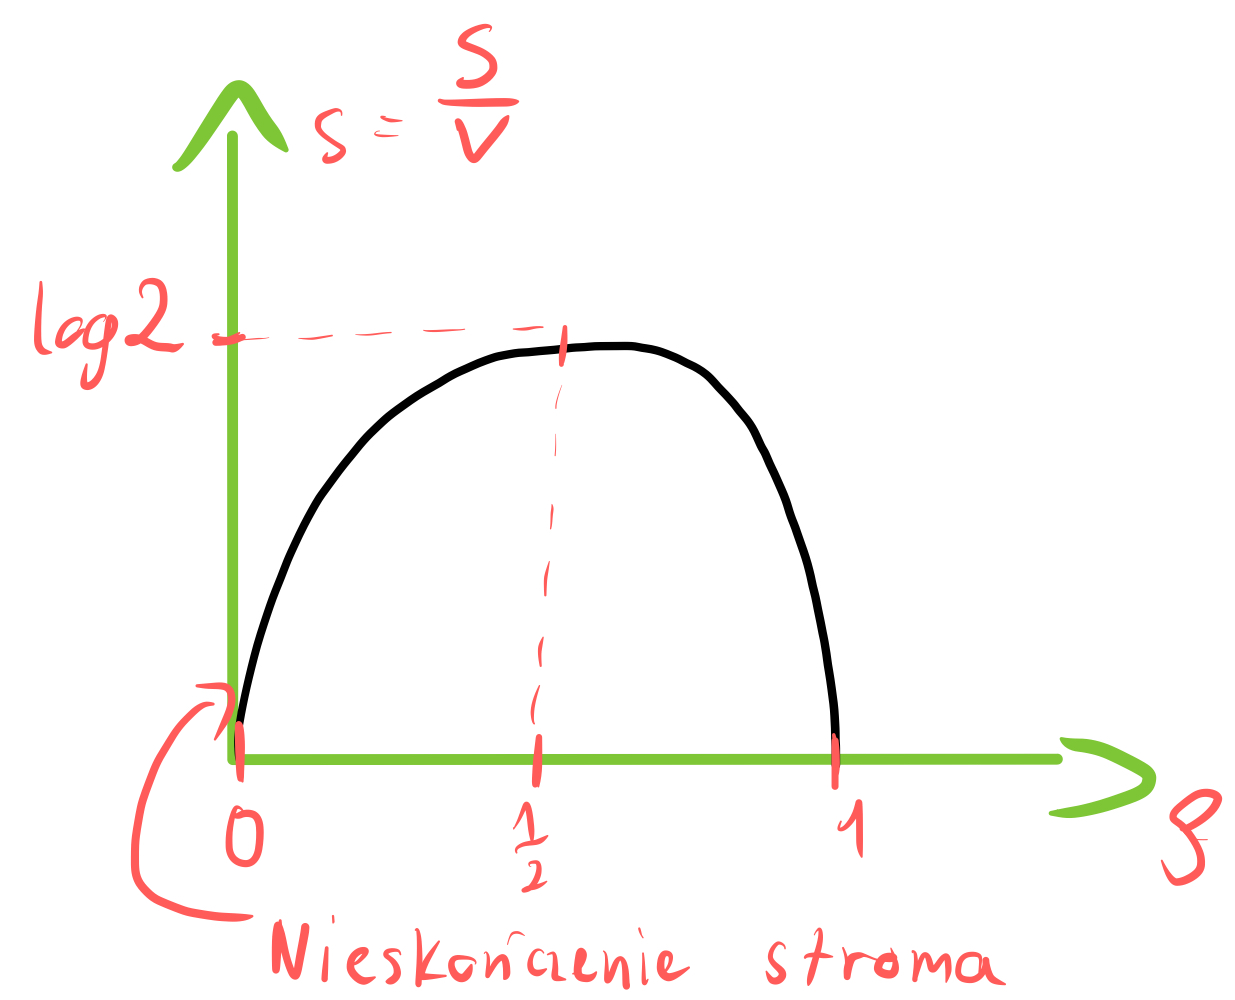
\includegraphics[width=0.5\linewidth]{Wyk_5_Rys_1.jpeg}
    \caption{Wykres entropii na jednostkę objętości w funkcji gęstości pcheł na Azorze}
    \label{fig:lec_5:entropia_plot}
\end{figure}

\section{Maksymalizacja Entropii}

Teraz dzieliimy sobie układ na dwie objętości: $V/2$ i $V/2$. Teraz niech $N_L$ - liczba z lewej, $N_P$ - liczba z prawej. Wtedy:
\begin{align*}
\varrho_L &= \frac{N_L}{V/2} & \varrho_P &= \frac{N_P}{V/2}\\
N_L &= \frac{V}{2} \varrho_L & N_P &= \frac{V}{2} \varrho_P\\
\end{align*}
Daje to:
\begin{align*}
    N_L + N_P = N\\
    \frac{V}{2} \varrho_L + \frac{V}{2} \varrho_P = V \varrho\\
    \varrho_L + \varrho_P = 2 \varrho
\end{align*}

Weźmy:
\[
    \log \Sigma = \log \mqty(V/2 \\ N_L) \mqty(V/2 \\ N_P) = \log \frac{\frac{V}{2}}{\qty(\frac{V}{2} \varrho_L)! \qty(\frac{V}{2} (1- \varrho_L))!} \frac{\frac{V}{2}}{\qty(\frac{V}{2} \varrho_L)! \qty(\frac{V}{2} (1- \varrho_P))!} = \dots\footnote{Po dokładny rachunek patrz załącznik \ref{fig:lec_5:app:maksymalizacja_entropii}} = 0
\]

Czyli wiemy, że:
\begin{align*}
    No.1 &= \frac{V}{2} (- \varrho_L \log \varrho_L - \frac{V}{2} (1 - \varrho_L \log (1 - \varrho_L))) \qc & No.2 &= \frac{V}{2} (- \varrho_P \log \varrho_P - (1 - \varrho_P \log (1 - \varrho_P)))
\end{align*}
Czyli:
\[
    S = k \frac{V}{2} \qty[\varrho_L \log(\varrho_L) - (1 - \varrho_L) \log(1 - \varrho_L) - \varrho_P \log(\varrho_P) - (1 - \varrho_P) \log(1 - \varrho_P))]
\]
Dalej daje to:
\begin{equation}
    \dv{S}{\varrho_L} = - k \frac{V}{2} \log\qty{\frac{\varrho_L (1 - 2 \varrho + \varrho_L)}{(1 - \varrho_L)(2 \varrho - \varrho_L)}} = 0
    \label{eq:lec_5:ds_drho}
\end{equation}
\[
    \varrho_L (1 - 2 \varrho + \varrho_L) = (1 - \varrho_L)(2 \varrho - \varrho_L) \implies
\]
\[
    \varrho_L = \varrho_R = \varrho
\]

Teraz sprawdźmy ze wzoru na pochodną \eqref{eq:lec_5:ds_drho} co sie stanie jak $\varrho_L = \varrho + \Delta \varrho$ i $\varrho_R = \varrho - \Delta \varrho$:

\[
    \dv{S}{\varrho_L} = -\frac{k V}{2} \log\qty{\frac{(\varrho - \Delta \varrho)(1 - \varrho) - \Delta \varrho}{(\varrho + \Delta \varrho)(1 - \varrho) + \Delta \varrho}}
\]
Czyli wtedy entropia maleje.

\wniosek Entropia (maksymalna liczba konfiguracji) jest maksymalizowana tylko i wyłącznie gdy $\varrho_L = \varrho_R$

\end{lecture}

% ------------------------------------------------------------------------
% Wykład 17.03.2022

\begin{lecture}{Entropia Gazu doskonałego, Termometr}
    \section{Przeniosło time}
    \subsection{Ad poprzedni wykład}
    Weźmy układ jednorodny, tj. $\varrho = \frac{N}{V}$\\
    Przypomnijmy, że entropia to:
    \[
        S = \log\sum = - Vk\qty[\varrho \ln(\varrho) + (1-\varrho) \ln(\varrho)]
    \]
    Podzielmy układ na dwie części tak jak ostatnim razem, tj.
    \begin{align*}
    \varrho_L &= \frac{N_L}{V/2} & \varrho_P &= \frac{N_P}{V/2}\\
    N_L &= \frac{V}{2} \varrho_L & N_P &= \frac{V}{2} \varrho_P\\
    \end{align*}
    Daje to:
    \begin{align*}
        N_L + N_P = N\\
        \frac{V}{2} \varrho_L + \frac{V}{2} \varrho_P = V \varrho\\
        \varrho_L + \varrho_P = 2 \varrho
    \end{align*}
    \begin{align*}
    N_L + N_P = N\\
    \frac{V}{2} \varrho_L + \frac{V}{2} \varrho_P = V \varrho\\
    \varrho_L + \varrho_P = 2 \varrho
\end{align*}
Wracamy też do wzoru wyprowadzonego na poprzednim układzie:
\[
    S = k \frac{V}{2} \qty[\varrho_L \log(\varrho_L) - (1 - \varrho_L) \log(1 - \varrho_L) - \varrho_P \log(\varrho_P) - (1 - \varrho_P) \log(1 - \varrho_P))]
\]
Wyciągamy teraz wniosek, że entropia będzie maksymalizowana, gdy $\varrho_L = \varrho_R = \varrho$ i ma wartość $\log\varrho$

\com{Wstaw zdjęcia slajdów Przeniosły}

    \section{Wyprowadzenie wzoru na entropię gazu doskonałego}
    Weźmy sobie:
    \begin{align*}
        P(\text{mikrostan}) &= \frac{1}{E(E, N, V)}\\
        H(\underbrace{x_1, x_2, \dots, x_n, p_1, p_2 \dots, p_n}_{\Gamma_n}) &= E = const.\\
        \varrho(\Gamma_n) &= \frac{1}{\omega(E, N, V)\footnotemark} \delta(E - H(\Gamma_n, V))\\
        \omega(E, N, V) &= \int \delta(E - H(\Gamma_n, V)) \dd{\Gamma_n}\qq{gdzie:}\\ \hline \\
        \dd{\Gamma_n} = \frac{\dd[3N]{p} \dd[3N]{q}}{h^{3N}\footnotemark N!\footnotemark} &\qc \omega(E, N, V) = \pdv{\Omega}{E}\\
        \Omega(E) &= \int_{\epsilon < E} \omega(\epsilon, N, V) \dd{\epsilon} = \int_{H(\Gamma_N) < E} \dd{\Gamma_N}\\ 
        H = \frac{1}{2m}\qty(p_1^2 + p_2^2 + \dots +p_n^2) = E &\implies \qty(p_1^2 + p_2^2 + \dots +p_n^2) = (\sqrt{2 m E})^2\\
        \hline
    \end{align*}
    \addtocounter{footnote}{-1}
    \footnotetext{Liczba konfiguracji}
    \refstepcounter{footnote}
    \footnotetext{Stała Plancka}
    \refstepcounter{footnote}
    \footnotetext{Jest to istotne o tyle, że w tym $N!$ siedzi nasze przekonanie fundamentalne, że te cząstki są \emph{nierozróżnialne} i dopiero jak przez to podzielimy, to wzór na Entropię się zgodzi.}
    I teraz patrzymy sobie na wymiar jednostkowy stałej Plankcka (bo chcemy udowodnić, że tylko jak ona tam jest to działa). Stała Plancka to $h = \frac{E}{\nu} \qty[\frac{J}{1/s} = J \cdot s]$ i analogicznie iloczyn $p \cdot q = \qty[kg \cdot \frac{m}{s} \cdot m = J \cdot s]$ \\
    Idąc dalej w tym wyprowadzeniu mamy:
    \begin{align*}
        \Omega(E, N, V) &= \frac{\pi^{\frac{3N}{2}}}{\qty(\frac{3N}{2})!} \qty(2 m E)^{3N/2} \frac{V^N}{h^{3N}N!}\\
        \omega = \pdv{\Omega}{E} &=  \frac{\pi^{\frac{3N}{2}}}{\qty(\frac{3N}{2})!} \frac{V^N}{h^{3N}N!} \frac{3N}{2} E^{\frac{3N}{2} - 1} \\
        k\footnotemark \ln(\omega) &= N k \qty{\ln(\frac{V}{N}) + \frac{3}{2}\ln(\frac{E}{N}) + \frac52 + \frac32 \ln(\frac{4 \pi m}{4 h^2})}\\
        \text{Korzystamy }&\text{teraz ze wzoru Stirlinga i dostajemy Entropię:}
    \end{align*}
    \addtocounter{footnote}{-1}
    \footnotetext{Stała Boltzmanna}
    \begin{equation}
        S(E, V, N) = N k \qty[\ln(\frac{V}{2}) + \frac32 \ln(\frac{E}{N}) + S_0\footnotemark]
    \end{equation}
    \refstepcounter{footnote}
    \footnotetext{Ten czynnik przez lata umykał a jest esencją zrozumienia dziedziny}
    
    Teraz spójrzmy sobie na pochodną Entropii:
    \[
        \dd{S(E, V, N)} = \qty(\pdv{S}{E})_{V, N} \dd{E} + \qty(\pdv{S}{V})_{E,N} \dd{V} + \qty(\pdv{S}{N})_{E, V} \dd{N}
    \]
    
    Gdzie znaleziona tu wielkość $T$ znalezniona z równania $\pdv{S}{E} = \frac{1}{T}$ to \ind{Temperatura absolutna} - w skali Kelvina
    
    \com{Przeniosło poleca rozdiał o historii Termodynamiki z ksiązki prof. Wróblewskiego + wklej tu coś ze slajdów od Przeniosły}
    
    \begin{emph_box}{Zerowa zasada termodynamiki}
        Jeśli układy A i B mogące ze sobą wymieniać ciepło są ze sobą w równowadze termicznej, i to samo jest prawdą dla układów B i C, to układy A i C również są ze sobą w równowadze termicznej. \link{https://pl.wikipedia.org/wiki/Zerowa_zasada_termodynamiki}{Wikipedia}
    \end{emph_box}
    \section{Pokazy}
    \subsection{\ind{Termometr}}
    Z zerowej zasady termodynamiki wynika zasada działania termometru. Pierwszy termometr, który bierzemy pod uwagę, to \subind{Termometr gazowy}{Termometr!gazowy}, patrz Rys. \ref{fig:lec_6:term_1}.
    
    \begin{figure}[ht!]
         \centering
         \begin{subfigure}[b]{0.4\textwidth}
             \centering
             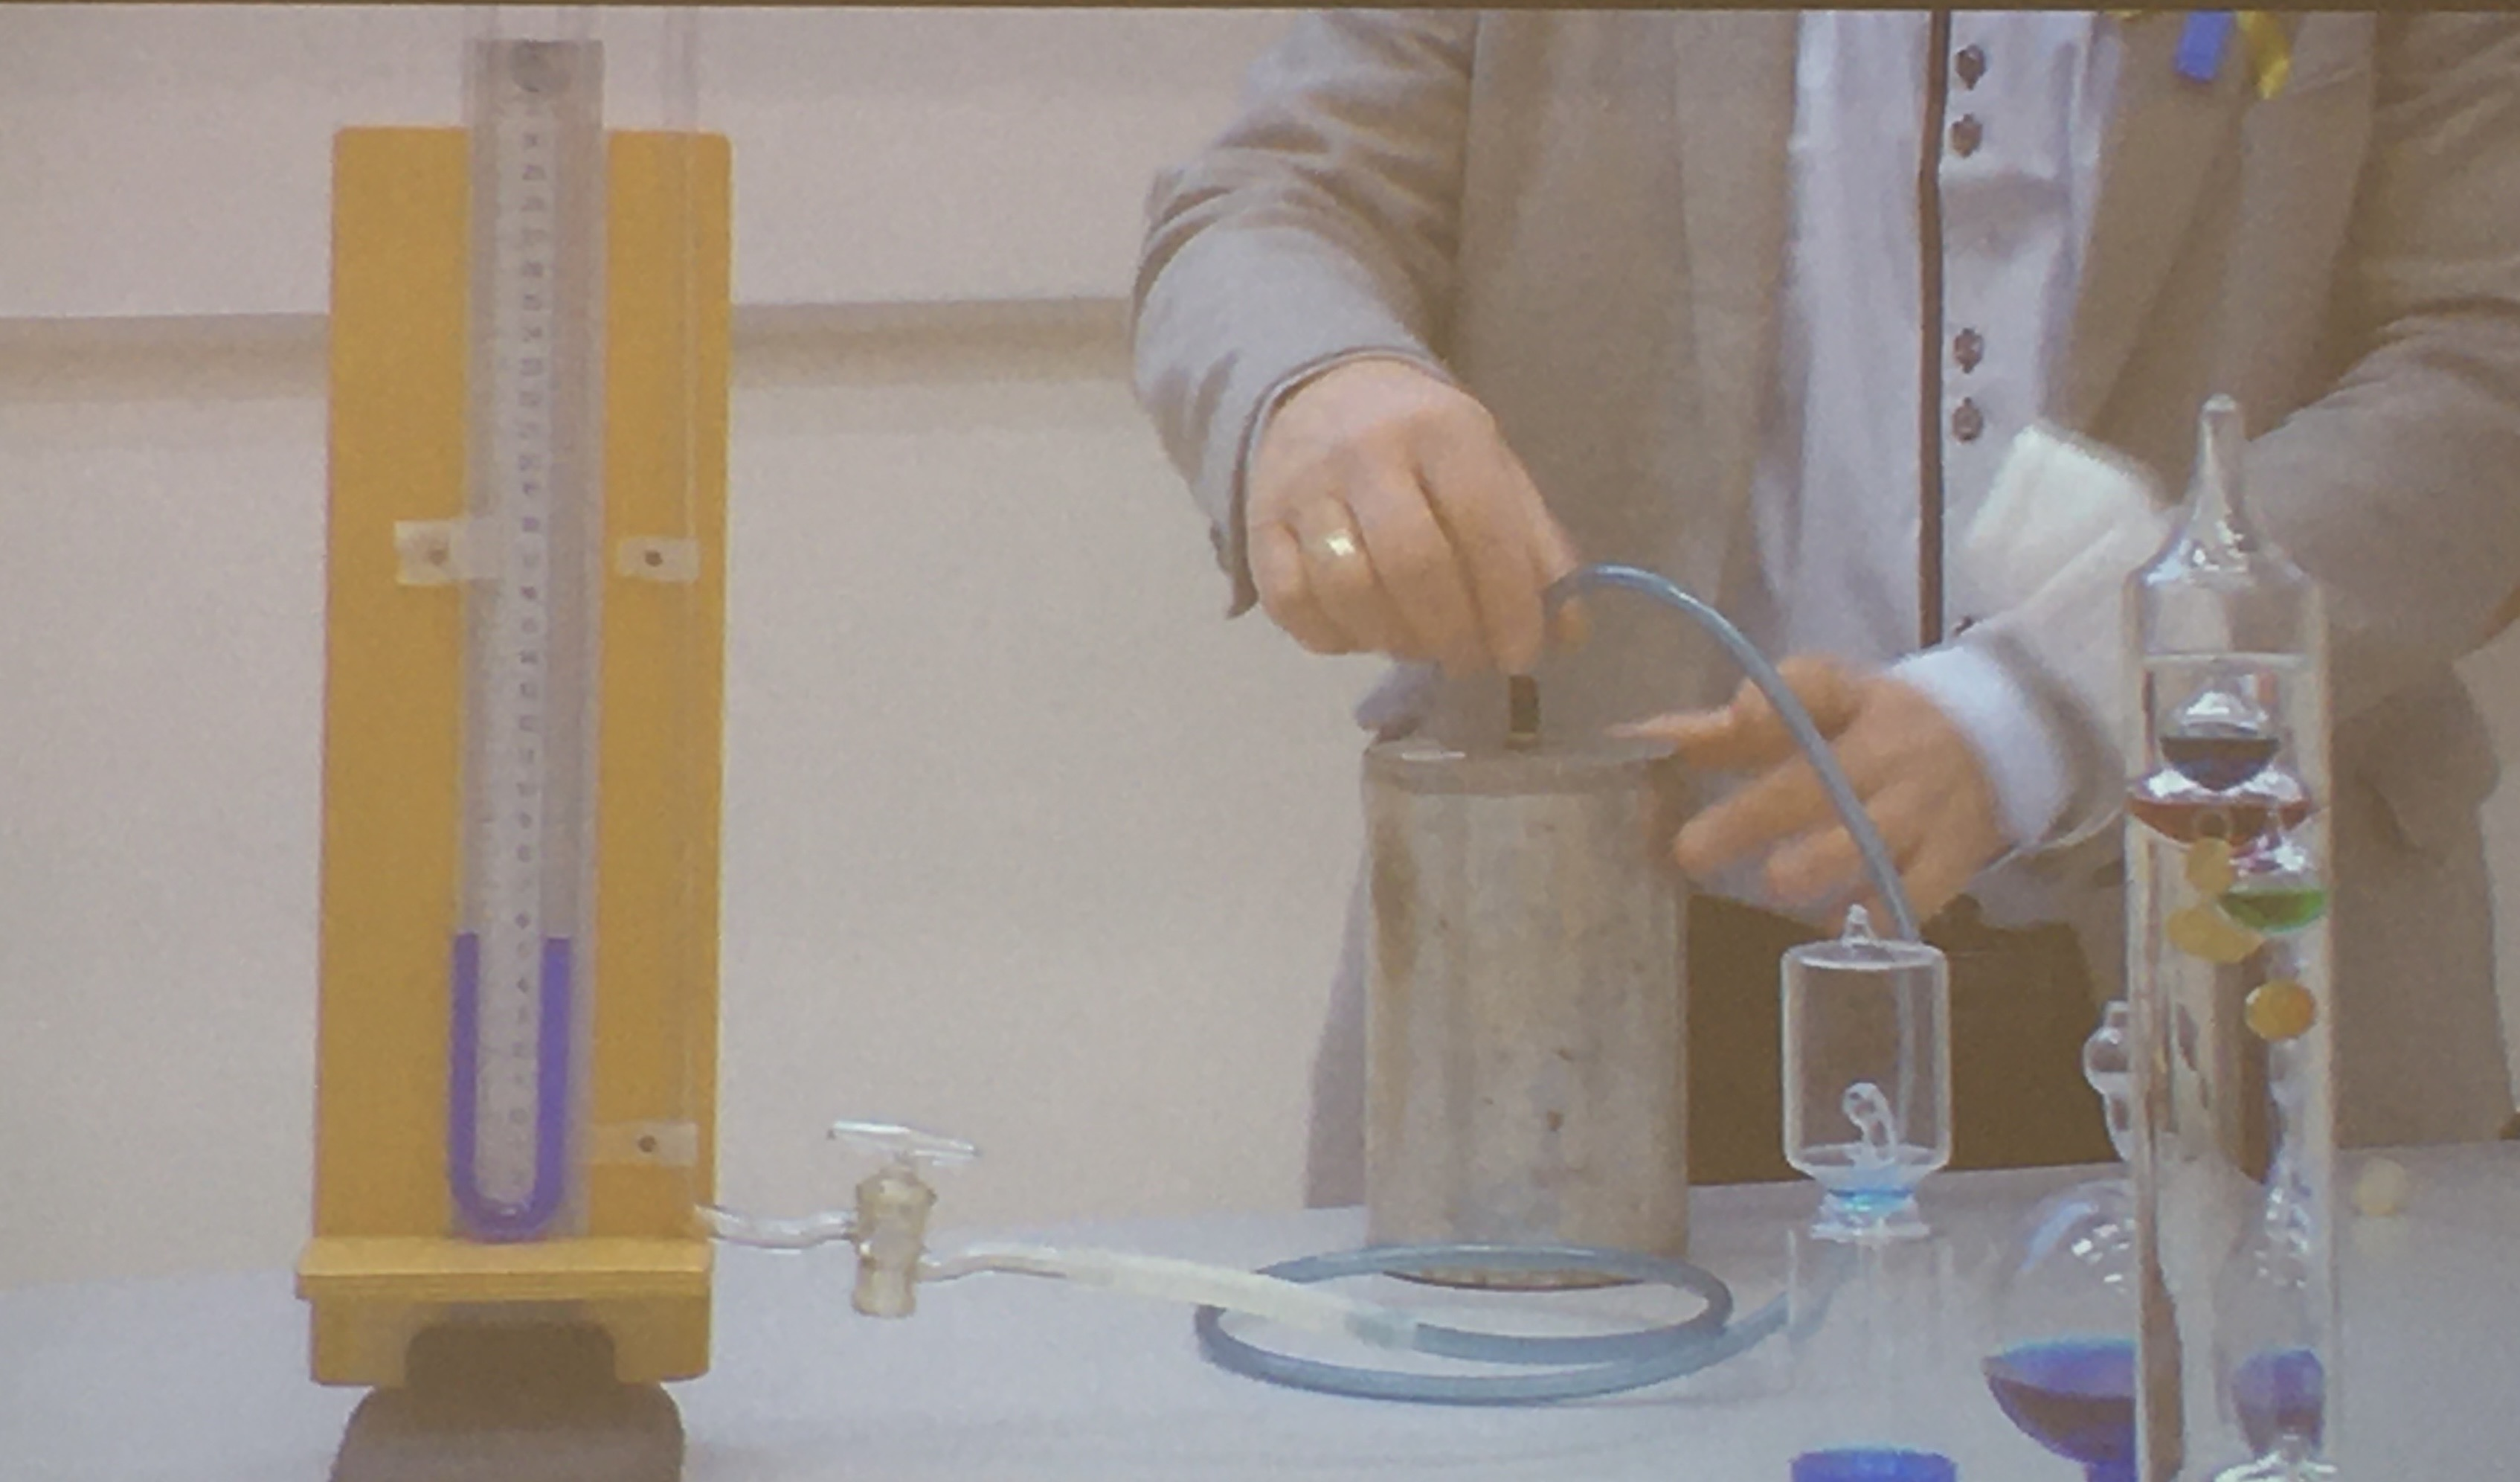
\includegraphics[width=\textwidth]{Wyk_6_Rys_1.JPG}
             \caption{Przed ogrzaniem}
             \label{fig:lec_6:term_1.1}
         \end{subfigure}
         \hfill
         \begin{subfigure}[b]{0.4\textwidth}
             \centering
             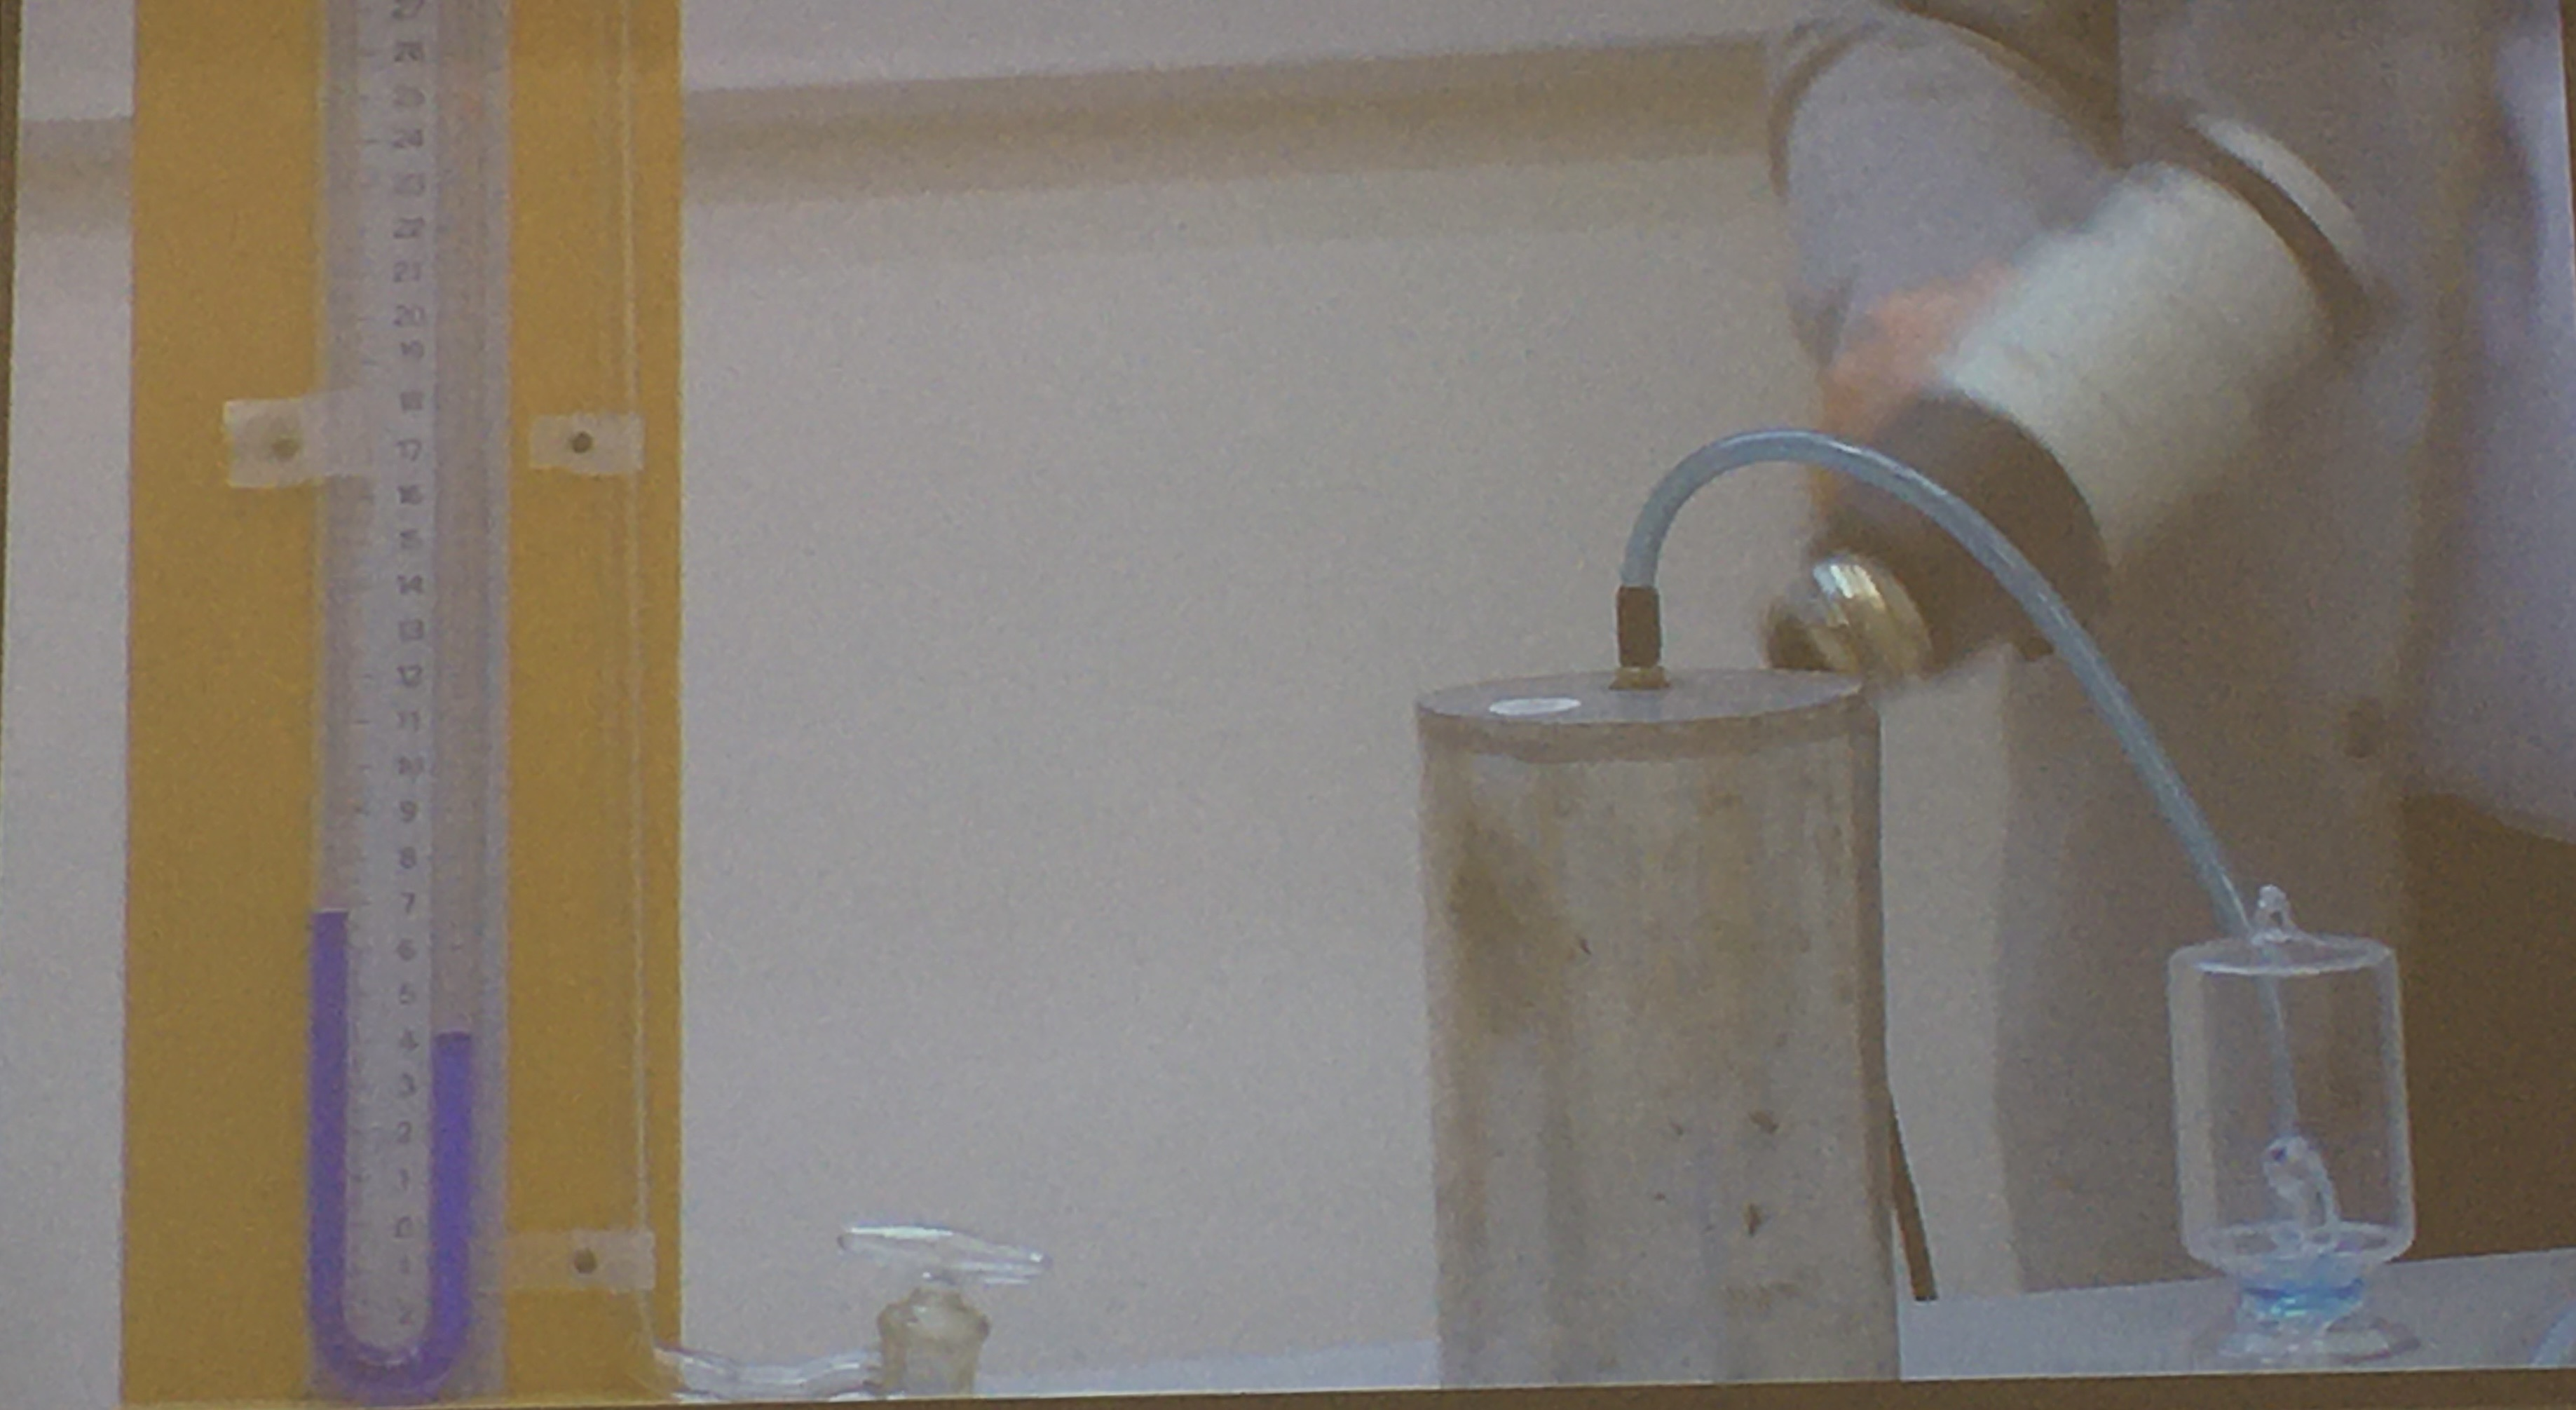
\includegraphics[width=\textwidth]{Wyk_6_Rys_2.JPG}
             \caption{Po ogrzaniu}
             \label{fig:lec_6:term_1.2}
         \end{subfigure}
        \caption{Termometr gazowy (tradycyjny) - rozszerzanie się parów gazu pod wpływem temperatury powoduje zmianę poziomu cieczy w pojemniku, co przekładamy na odczyt temperatury}
        \label{fig:lec_6:term_1}
     \end{figure}
    
    \com{Wstaw slajdy z prezentacji Przeniosły}\\
    Działają te termometry poprzez mierzenie w jakiś sposób zmiany objętości gazu który jest w układzie zamkniętym\\
    Dobrym ciałem/zjawiskiem wzorcowym do cechowania termometru {\color{orange} Nie jest} temperatura przejścia fazowego woda-lód, ani woda-gaz. Za to dobrym punktem {\color{orange} Jest} tzw. \ind{Punkt potrójny}, gdzie łączą się wszystkie przejścia fazowe. Dla wody jest to $273.17$K. \\
    Pokaz punktu potrójnego na bazie Bromu. \nameref{fig:lec_6:term_2}\\
        \begin{figure}[ht!]
         \centering
         \begin{subfigure}[b]{0.4\textwidth}
             \centering
             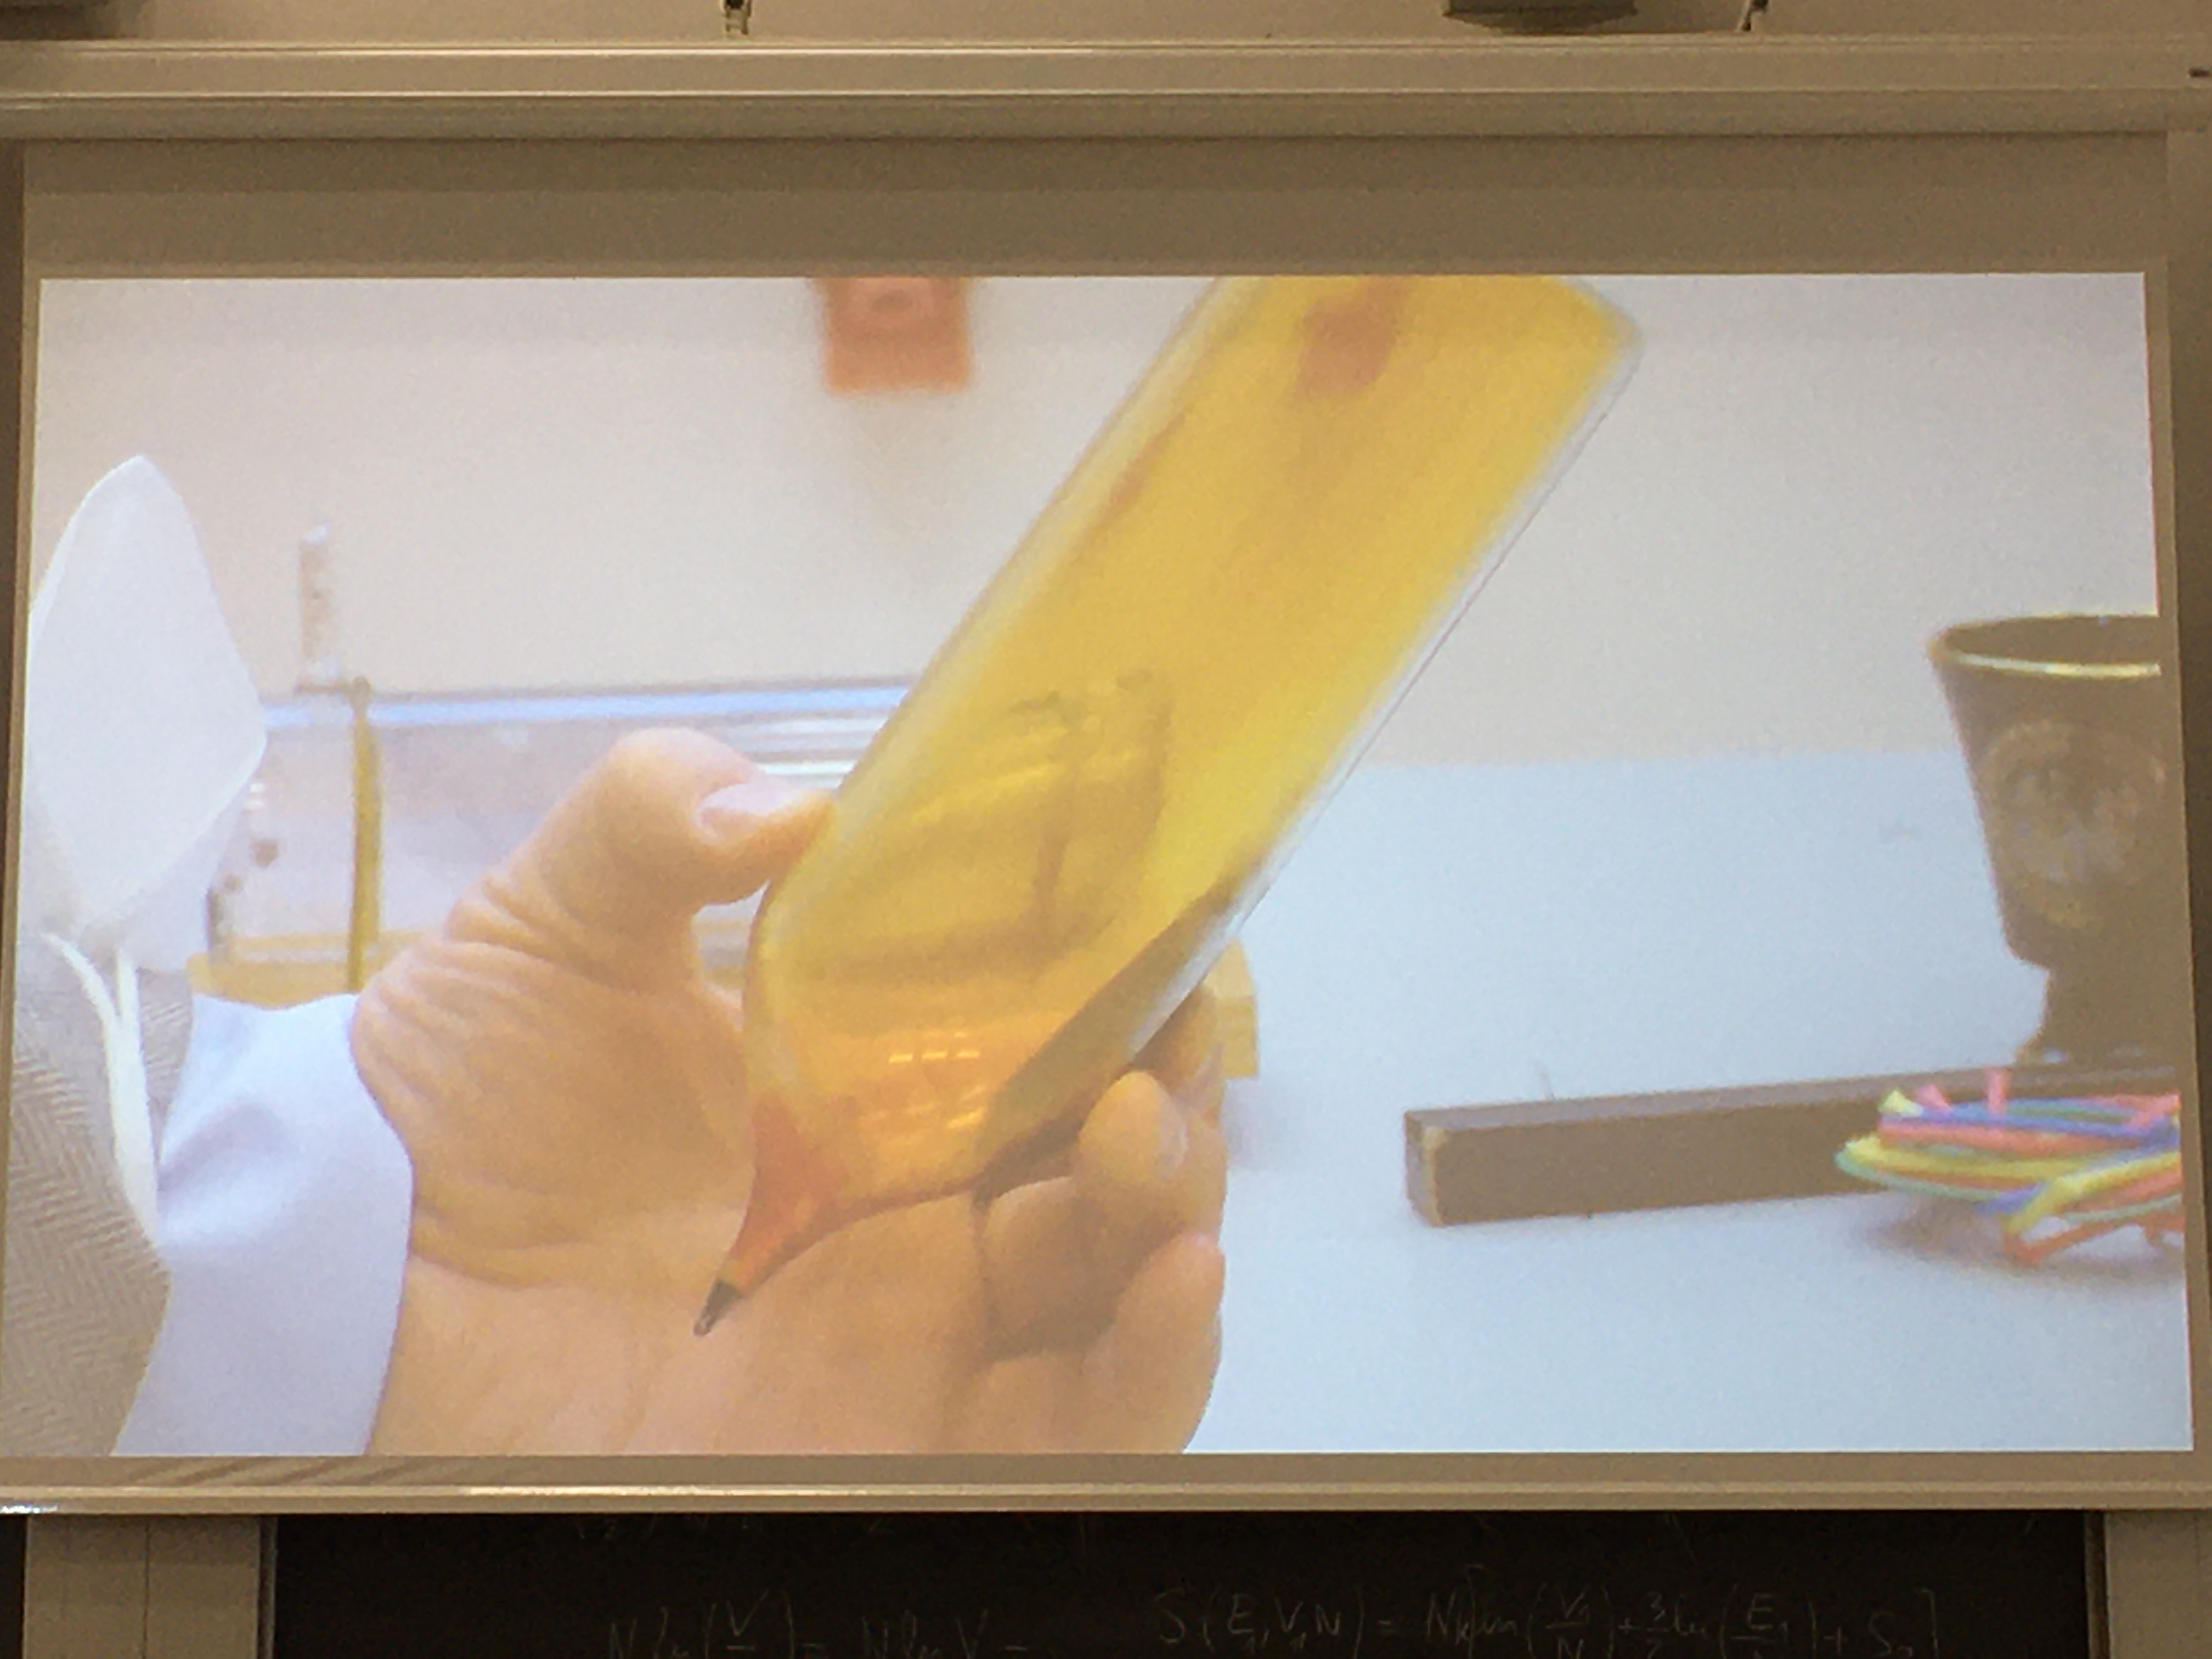
\includegraphics[width=\textwidth]{Wyk_6_Rys_3.JPG}
             \caption{Przed ogrzaniem}
             \label{fig:lec_6:term_2.1}
         \end{subfigure}
         \hfill
         \begin{subfigure}[b]{0.4\textwidth}
             \centering
             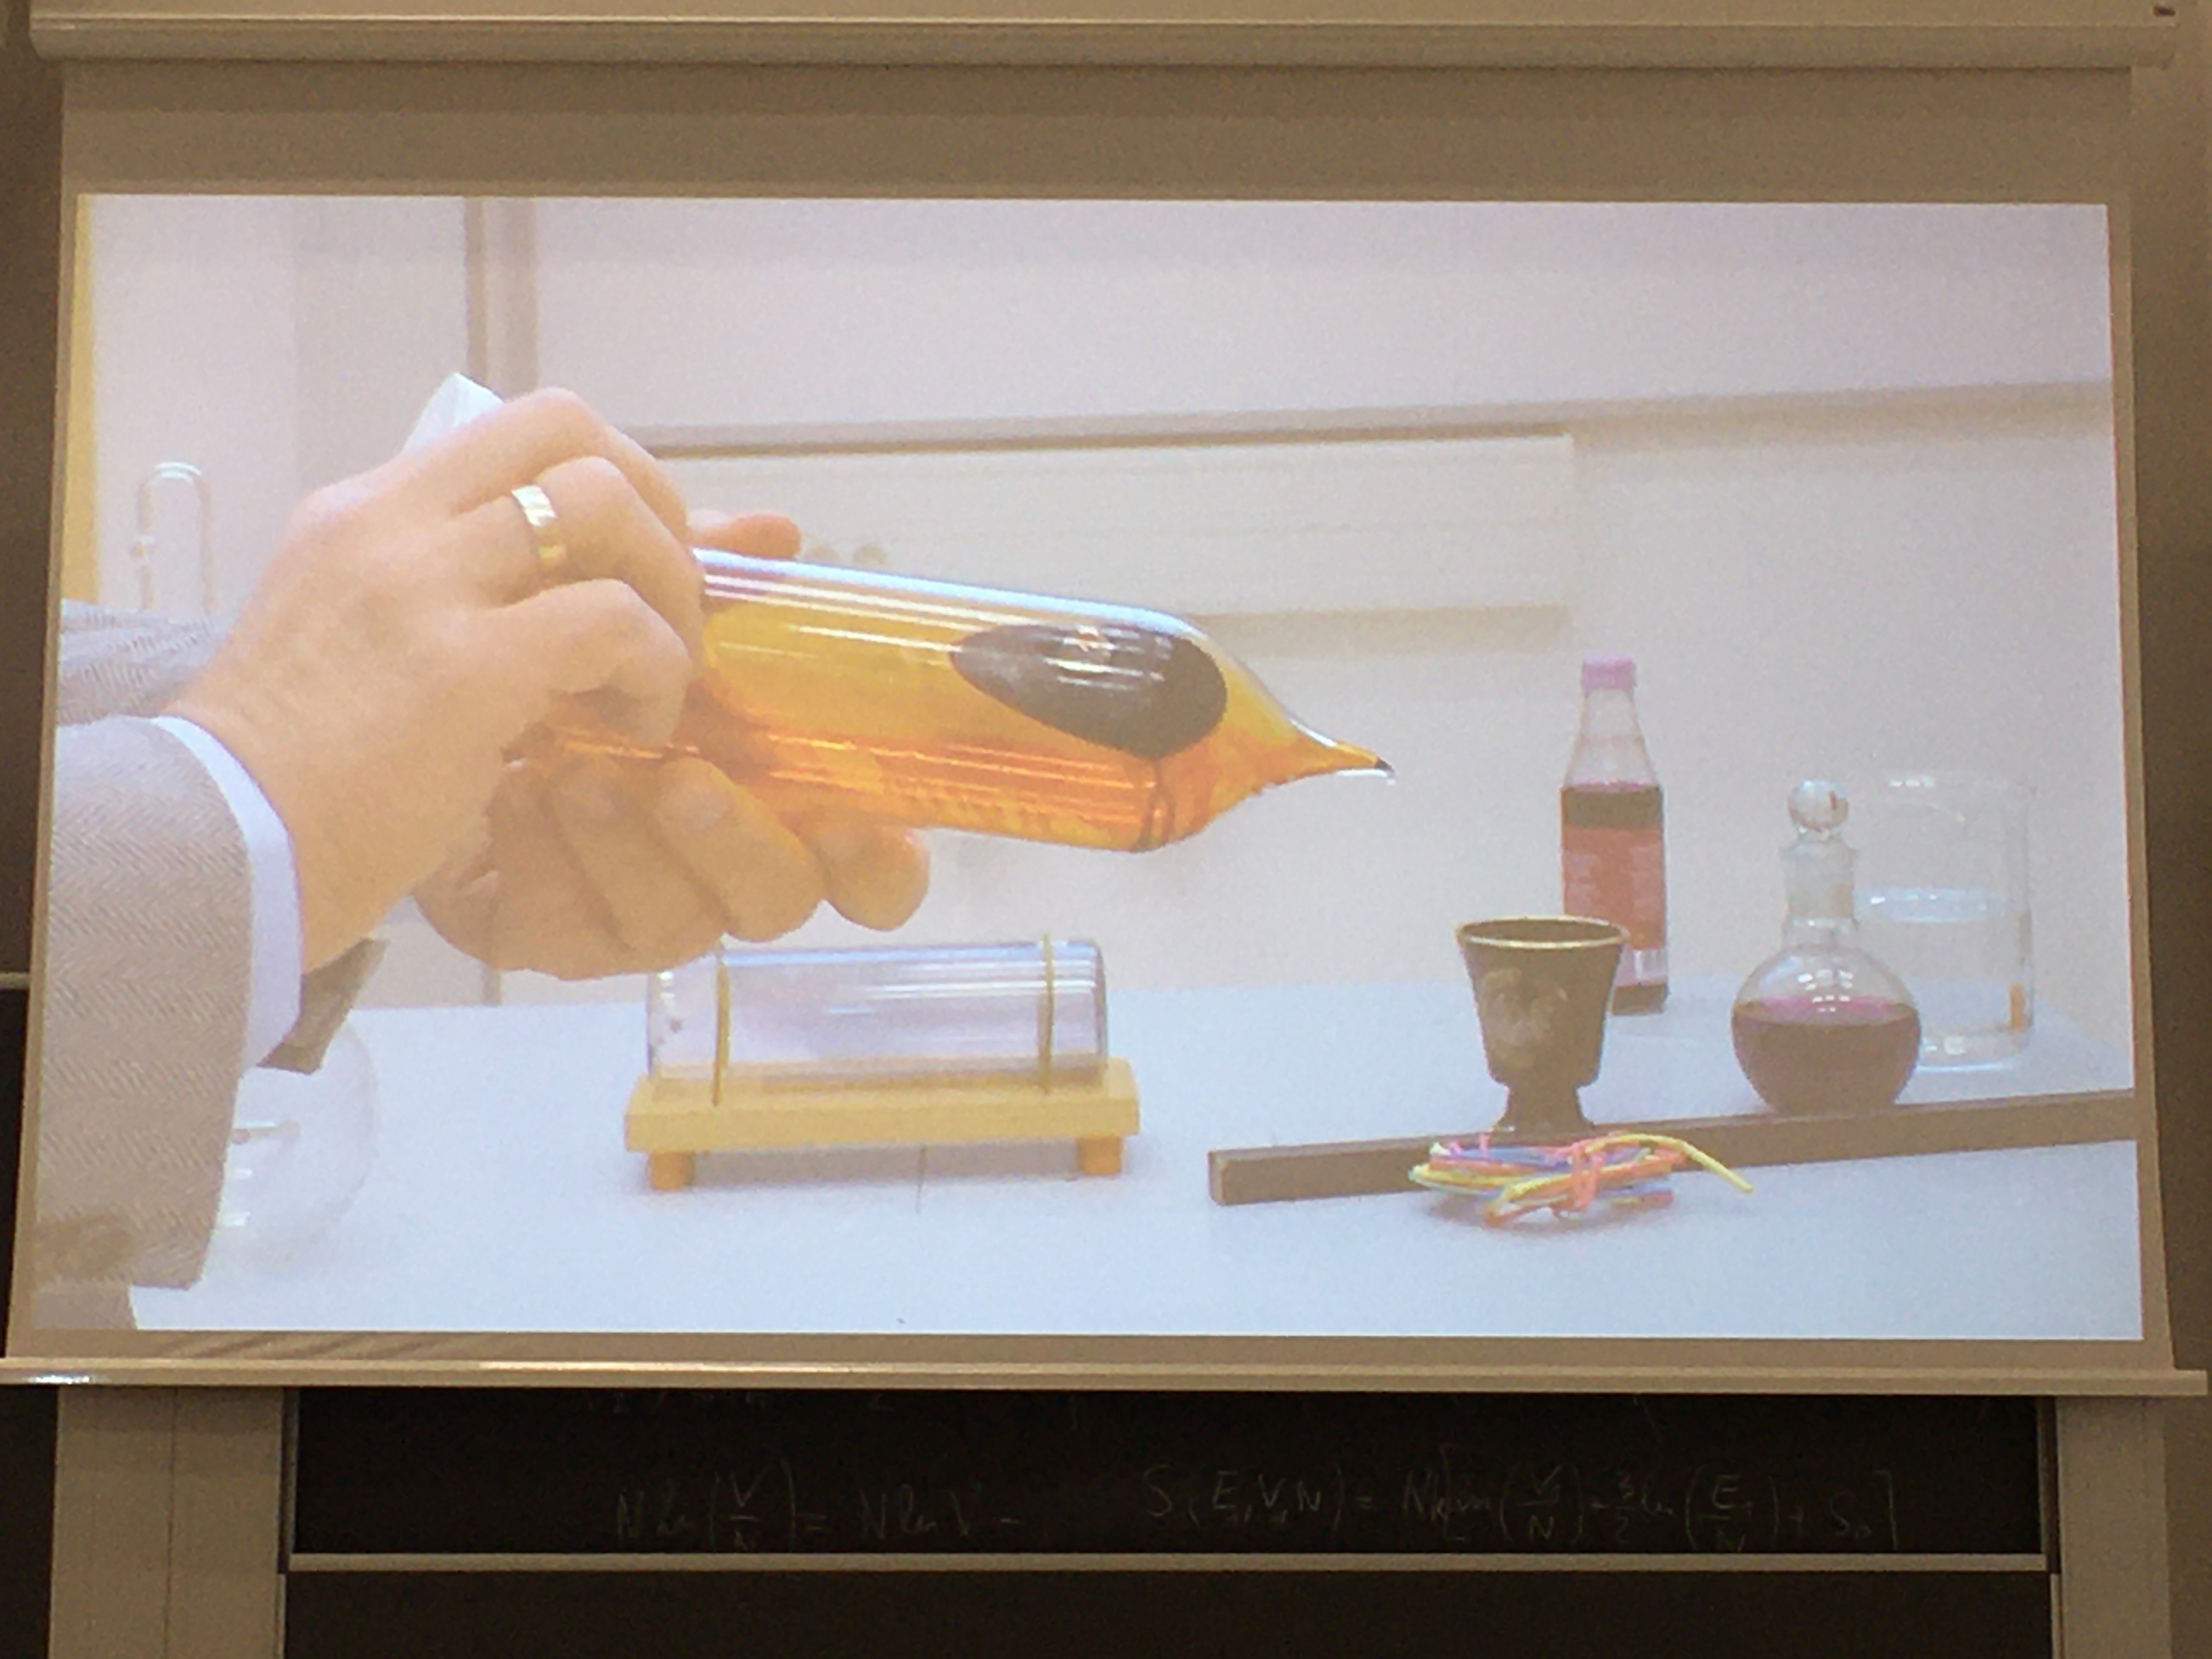
\includegraphics[width=\textwidth]{Wyk_6_Rys_4.JPG}
             \caption{Po ogrzaniu}
             \label{fig:lec_6:term_2.2}
         \end{subfigure}
        \caption{Na Rys. \ref{fig:lec_6:term_2.1} widać stan bańki z Bromem tuż po wyjęciu z zamrażarki, obecne są tylko pary Bromu (żółta para) i ciało stałe, a po ogrzewaniu pojawia się też i ciecz z topiącego się ciała stałego (Rys. \ref{fig:lec_6:term_2.2}). Wtedy Brom jest w okolicy swojego punktu potrójnego}
        \label{fig:lec_6:term_2}
     \end{figure}
    Żeby skala była dobra, to współczynnik termometryczny musi być liniową funkcją temperatury. Czyli np taka woda w zakresie $0-8$ stopni Celsiusza by się nie nadawała, bo ma w $4$ stopniach maksimum gęstości.\\
    Co ciekawe dla żelaza również nie jest to monotoniczna zależność gęstości od temperatury, bo jak się grzeje, to zachodzi przejście fazowe ok $500$ stopni, i ma dziwny przebieg przez to.\\
    Doświadczenie z kulką: Jak grzaliśmy otwór, to kulka wciąż przechodzi, ponieważ jak tempetarura rośnie, to rosną srednie odległości między atomami w obręczy, czyli otwór się \emph{powiększa}.

\end{lecture}

% ------------------------------------------------------------------------
% 21.03.2022

\begin{lecture}{Kij wie jaki temat}

\emph{Jachymski ma zastępstwo}

\com{Od Szymona}

\begin{align*}
	S &= k N \left[ \log \frac{V}{N} \left( \frac{4 \pi m}{3 h^2} \frac{E}{N} \right)^{3 /2}  + \frac{5}{2}  \right]  \\
\end{align*}
dla gazu doskonałego. Pudełko z gazem opisują dla nas 4 wartości: energia $E$, objętość $V$, liczba cząsteczek $N$ i entropia $S$. Wypisaliśmy również wzór na temperaturę związany z entropią, ale nie był zaargumentowany. \\

Przedzielmy pudełko ścianką, która pozwala na przepływ energii. Ale liczba cząstek się nie zmienia. Pierwsza część w czasie $t=0$ ma energię $E_1'$ a druga $E_2'$, w stanie równowagi $t \to \infty$ mamy $E_1, \, E_2$ oraz cała energia jest zachowana $E_1+ E_2 = E_1' + E_2' = E$. \\
Entropia się jednak zwiększy. W stanie równowagi powinna być maksymalna. Co to znaczy, że entropia jest maksymalna?
\begin{align*}
	\delta S &=  \pdv[]{S_1}{{E_1}} \delta E_1 + \pdv[]{S_2}{{E_2}} \delta E_2, \\
	\intertext{Natomiast $\delta S_1 = - \delta S_2$. Co za tym idzie, $\pdv*[]{}{{E_1}} = - \pdv*[]{}{{E_2}} $. Entropia ma się nie zmieniać, mamy więc wniosek}
	\frac{1}{T} &\coloneq \pdv[]{S_1}{{E}} = \pdv[]{S_2}{{E}} 
\end{align*}
Weźmy wycinek z dochodzenia układu do położenia równowagi. W pewnym momencie będziemy mieli energie $E_1 + \Delta E $ i $E_2 - \Delta E$. Wówczas,
\begin{align*}
	\Delta S &= \pdv[]{S_1}{{E_1}} \Delta E - \pdv[]{S_2}{{E_2}}  \Delta E = \left( \frac{1}{ T_1} - \frac{1}{T_2} \right) \Delta E  
\end{align*}
$\Delta S >0$, mamy więc dwa przypadki.
\begin{enumerate}
	\item $\displaystyle{\Delta E >0, \quad \frac{1}{T_1} - \frac{1}{T_2} >0}$, wówczas $T_1 < T_2$
	\item $\Delta E < 0$, wówczas $T_1 > T_2$. 
\end{enumerate}
Zatem widzimy, że przy tej definicji energia przepływa z układu o większej temperaturze do układu o mniejszej temperaturze. To jest to co byśmy chcieli. \\

Możemy więc teraz policzyć temperaturę gazu doskonałego. Niech $s = S / N$ i podobnie pozostałe wartości przeskalujmy przez liczbę cząstek.
\begin{align*}
	s &= k \left[ \log v + \frac{3}{2} \log \varepsilon + \frac{5}{2} + \frac{3}{2} \log \frac{4 m \pi }{3 h^2} \right]  \\
	\frac{1}{T} &= \pdv[]{s}{{\varepsilon}} = \frac{3}{2} \frac{k}{\varepsilon} 
\end{align*}
Stąd otrzymujemy znane wzory na związek energii gazu z jego temperaturą. 
\begin{align*}
	\varepsilon &= \frac{3}{2} k T \\
	E &= \frac{3}{2} N kT 
\end{align*}

% -----
% Zredaguj powyżej

Na ostatnim wykładzie pojawiła się Entropia gazu doskonałego:
\begin{equation*}
        S(E, V, N) = N k \qty[\ln(\frac{V}{2}) + \frac32 \ln(\frac{E}{N}) + S_0]
\end{equation*}
Stan gazu jest opisywany czterema wartościami:
\begin{itemize}
    \item Energią $E$
    \item Objętością $V$
    \item Ilością cząstek $N$
    \item Entropią $S$
\end{itemize}

Będziemy sobie teraz przedzielać pudełko ściankami o różnych właściwościach

Wypisaliśmy wzór Sackur-Tetrodre:
\[
    S = k N \qty(\log\frac{V}{N}\qty(\frac{4 \pi m E}{3 h^2 N})^{\frac32} + \frac52)
\]

\com{Przepisz z tych 10 min}

\section{Zależność od energii, entropii i temperatury}

Teraz rozważmy sobie układ, pudełko zamknięte tłokiem o masie $m$, wysokości $h$, powierzchni $A$, w polu $g$. \com{Wstaw rysunek}.Zajdą zależności:
\begin{align*}
    E &= E_g + mhg\\
    S &= k \log \sum(E_g, V) = k \log \sum (E - mgh, Ah)
\end{align*}
Stan równowagi osiągniemy, gdy $\pdv{S}{h} = 0$:
\begin{align*}
    \pdv{S}{h} &= 0\\
    \pdv{S}{h} = k \pdv{\log \Sigma}{E_g} \pdv{E_g}{h} + \pdv{\log \Sigma}{V} \pdv{V}{h} &= - k mg \pdv{\log \Sigma}{E_g} + k A \pdv{\log \Sigma}{V}\\
    0 = - mg\qty(\pdv{S}{E_g})_V + A \qty(\pdv{S}{V})_{E_g} &\implies \qty(\pdv{S}{V})_{E} = \frac{m g}{A T} = \frac{p}{T}
\end{align*}

Teraz rozważmy sobie układ, gdzie ścianka między pojemnikami z dwoma gazami jest ruchoma. Mamy więc więc pojemniki o objętościach $V_1$ i $V_2$. Teraz szukając stanu równowagi dostajemy:
\begin{align*}
    \pdv{S}{V_1} = 0 \qc \pdv{S}{E_1} = 0 \implies T_1 = T_2\\
    \pdv{S}{V_1} = \pdv{S_1}{V_1} - \pdv{S_2}{V_1}\\
    \implies \pdv{S_1}{V} = \pdv{S_2}{V}\qc p_1 = p_2 \qc \frac{p_1}{T_1} = \frac{p_2}{T_2}
\end{align*}

Spójrzmy teraz na małą zmianę Entropii:
\[
    \Delta S = \pdv{S_1}{V_1} \Delta V - \pdv{S_2}{V_2} \Delta V = \qty(\frac{p_1}{T_1} - \frac{p_2}{T_2}) \Delta V = \qty(\frac{p_1 - p_2}{T})\Delta V > 0
\]
Czyli $\Delta V > 0 \implies p_1 > p_2$. Patrzymy teraz na entropię:
\(
    s = k (\log v + \dots) \implies \pdv{s}{v} = \frac{k}{v}
\) Daje to: \( p = \frac{kT}{p} \implies pV = NkT \)
\begin{emph_box}{Wzór Clapeyrona}
    \[
        pV = NkT
    \]
\end{emph_box}

Rozważamy teraz \emph{ściankę adiabatyczną} (termos):
\com{Rysunek}
W tym przypadku mamy;
\[ 0 = 
  \begin{cases}
      \Delta V\\
      \Delta E\\
      \Delta N
  \end{cases}
\]
Czyli inaczej mówiąc wymiana ciepła z otoczeniem nie zachodzi.

\section{Pokazy}
\emph{Zależność ciśnienia od głębokości w cieczy}

\com{Wstaw zdjęcie z ururką i balonem}
Patrząc na doświadczenie widzimy, że rurka z cieczą jest z jednej strony otwarta, a z drugiej zamknięta balonikiem, który jest wsuwany wgłąb cylindra z wodą. Wzrost ciśnienia działającego na balon obserwujemy poprzez to, że poziom cieczy w rurce się zmienia wraz ze wsuwaniem balonika na głębokość\\
\com{Zdjęcie implozji puszki}\\

\emph{Pokazy z różnicą ciśnień (Efekt wysokogórski etc.)} \com{Zdjęcia i film} \com{Zdjęcie z wodą wrzącą w temperaturze pokojowej w niskim ciśniniu}\\

\emph{Pokaz z zamrażaniem lodu poprzez gwałtowne zmiejszenie ciśnienia w układzie z wodą}

Ciecz która jest pomiędzy wodą a pompą to kwas siarkowy, który jest silnie higroskopijny, więc dzięki temu odfiltrowujemy powietrze od wody i zyskujemy efekt obniżenia temperatury wody i zamarzania. 

\emph{Nurek Kartezjusza} \com{Zdjęcia}\\
W nurku jest stała ilość gazu zamknięta w szklanej bańce powietrza. Od dołu jest otwarta ta bańka, wiec jest zatknięta wodą. Zwiększajac ciśnienie wody powietrze się spręża co raz bardziej, więc siła wyporu spada, a siła grawitacji pozostaje bez zmian bo jest niezależna od objętości gazu i nurek tonie. Jak zmniejszamy ciśnienie, to nurek się na nowo wynurza.

\section{Powrót do teorii}
Ostatni rodzaj ścianki, pozwala na przepływ energii i cząstek ale nieruchoma (ścianka wyimaginowana)
Czyli mamy:
\[
    const = 
    \begin{cases}
    N_1 + N_2 = N\\
    E_1 + E_2 = E
    \end{cases}
\]
Oraz wiemy, że:
\begin{align*}
    0 = \pdv{S}{N_1} = \pdv{S_1}{N_1} - \pdv{S_2}{N_2} &\implies \qty(\pdv{S}{N})_E = - \frac{\mu}{T}\\
    \text{Mała zmiana }&\text{entropii}:\\
    \Delta S = \pdv{S_1}{N_1}\Delta N = \pdv{S_2}{N_2}\Delta N &= \frac{\mu_1 = \mu_2}{T} \Delta N > 0\\
    \implies \Delta N>0\implies&\mu_1 < \mu_2
\end{align*}
Gdzie wielkość $\mu$ to \ind{Potencjał Chemiczny} - możemy go rozumieć jako 'chęć' cząstek do przechodzenia między dwoma objętościami.

\end{lecture}

% ------------------------------------------------------------------------
% 24.03.2022

\begin{lecture}{Potencjał chemiczny}

\section{Potencjał Chemiczny Gazu Doskonałego}
Piszemy równanie na Entropię:
\[
    S = k N (\ln V + \frac32 \ln \frac{4 \pi m}{3 h^2} + \frac52 + \frac32 \ln E - \frac52 \ln N)
\]
Wtedy \subind{potencjał chemiczny}{Potencjał Chemiczny} będzie wyglądać:
\[
    \mu = \frac{S}{N} - \frac52 k = - k T \qty(\ln\qty(\frac{V}{N}\qty(\frac{2 \pi n k T}{h^2})))
\]


\section{Warunki nieidealne}
Do tej pory braliśmy tylko układy odizolowane o parametrach $E, N, V, S, T, \mu, p$, ale IRL nasz układ o stanie $\mathbb{S}$ jest w jakimś rezerwuarze $R$. Wtedy Energia całkowita to będzie:\\
$E = E_S + E_R$ - suma energii układu o stanie $\mathcal{S}$ i rezerwuaru $R$.\\
Oznaczamy to jako $\Gamma_N = \qty{\Gamma_S, \Gamma_R}$ - Stan układu $R+S$. Rozpiszemy to jako:
\[
    \rho(\Gamma_N) = \frac{1}{\omega(E, V, N)} \delta(E - H(\Gamma_N)) 
\]
Weźmy teraz $\varrho = \rho(\Gamma_S, \Gamma_R)$. Wtedy:
\[
    \rho_S(\Gamma_S) = \int\dd{\Gamma_R} \varrho(\Gamma_S, \Gamma_R) = \int \dd{\Gamma_R} \frac{1}{\omega} \delta(E - H_S(\Gamma_S) - H_R(\Gamma_R))
\]
\[
    \rho_S(\Gamma_S) = \frac{1}{\omega(E, V, N)} \omega_R(E - H_S(\Gamma_S), V_R, N_R)
\]
Pamiętając, że:
\[
    \mqty{
        \omega = \int \delta(E - H(\Gamma)) & \omega = e^{\frac{S}{k}}\\
        k \log \omega = S
    }
\]
Stosując te założenia do poprzednich wzorów:
\[
    \rho_S(\Gamma_S) \sim e^{\frac{1}{k} S_R(E - E_S, V_R, N_R)}
\]
Dalej zakładamy $\abs{S} \ll \abs{R}$, $\abs{E_S} \ll \abs{E}$. Rozwijamy wokół $E_S = 0$
\[
    S_R(E-E_S, V_R, N_R) \approx S_R(E) - \pdv{S_R}{E} E_S
\]
Z normalizacji $\rho_S$, biorąc $\beta = \frac{1}{k T}$:
\[
    \mqty{
    \rho_S = \frac{1}{Z} e^{- \beta E_S(\Gamma_S)}\\
    Z = \int\dd{\Gamma_S} e^{-\beta E(\Gamma_S)}
    }
\]
Gdzie wielkosć 
\begin{equation}
    Z = \int\dd{\Gamma_S} e^{-\beta E(\Gamma_S)}
    \label{eq:lec_8:suma_stat}
\end{equation}
nazwiemy \subind{sumą statystyczną}{Suma Statystyczna}, zaś wielkość $Z(T, V, N)$ nazwiemy \subind{zespołem kanonicznym}{Zespół Kanoniczny}

Idąc dalej mamy:
\begin{align}
    \ev{E} &= U = \int_\Gamma E(\Gamma) \rho(\Gamma) \dd{\Gamma} = \\
    &= \frac{1}{Z(T, V, N)} \int E e^{- \beta E(\Gamma)} \dd{\Gamma} = - \frac{1}{Z}\pdv{\beta}\int e^{- \beta E(\Gamma)} \dd{\Gamma} = \\
    &= -\frac{1}{Z} \pdv{Z}{\beta} = - \pdv{\log Z}{\beta}
\end{align}
Licząc sobie teraz dyspersję tego rozkładu:
\begin{align}
    \ev{(\Delta E)^2} &= \ev{E^2} - \ev{E}^2\\
    \ev{E} &= \footnotemark
\end{align}
\begin{figure}[ht!]
         \centering
         \begin{subfigure}[b]{0.4\textwidth}
             \centering
             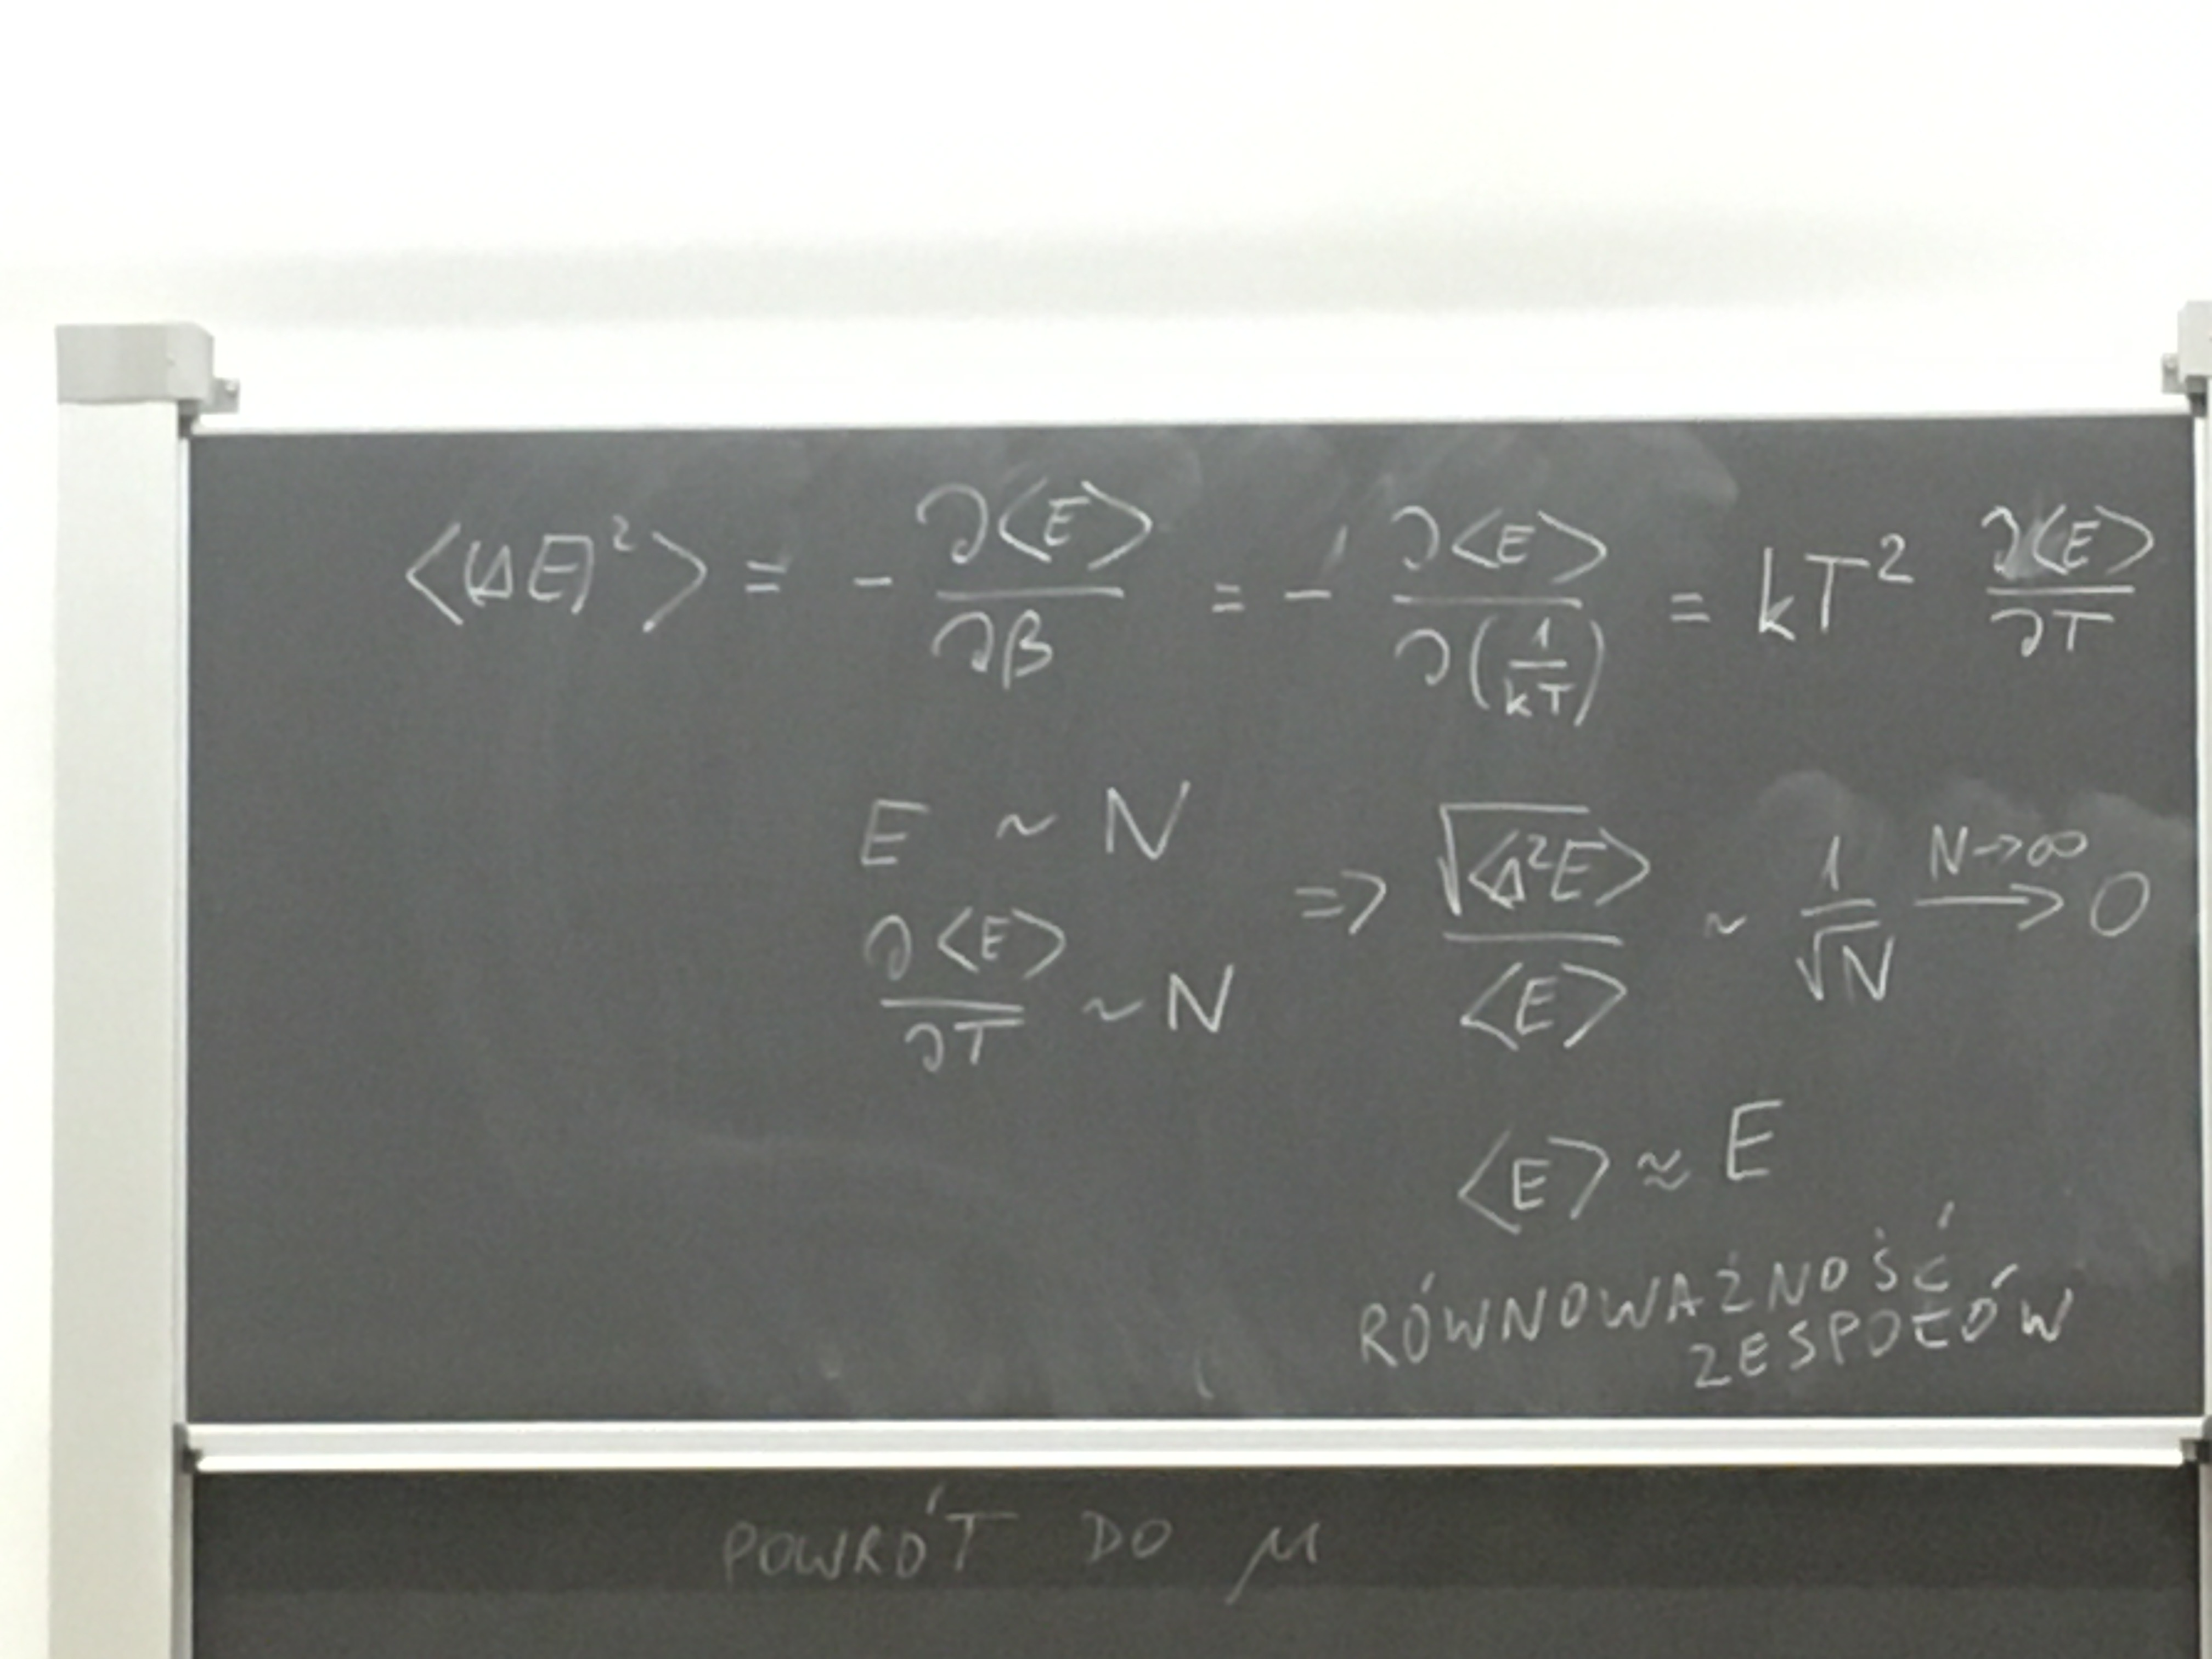
\includegraphics[width=\textwidth]{Wyk_8_Rys_1.JPG}
             \caption{Pierwsza część wyprowadznia}
             \label{fig:lec_8:do_przepisania_1.1}
         \end{subfigure}
         \hfill
         \begin{subfigure}[b]{0.4\textwidth}
             \centering
             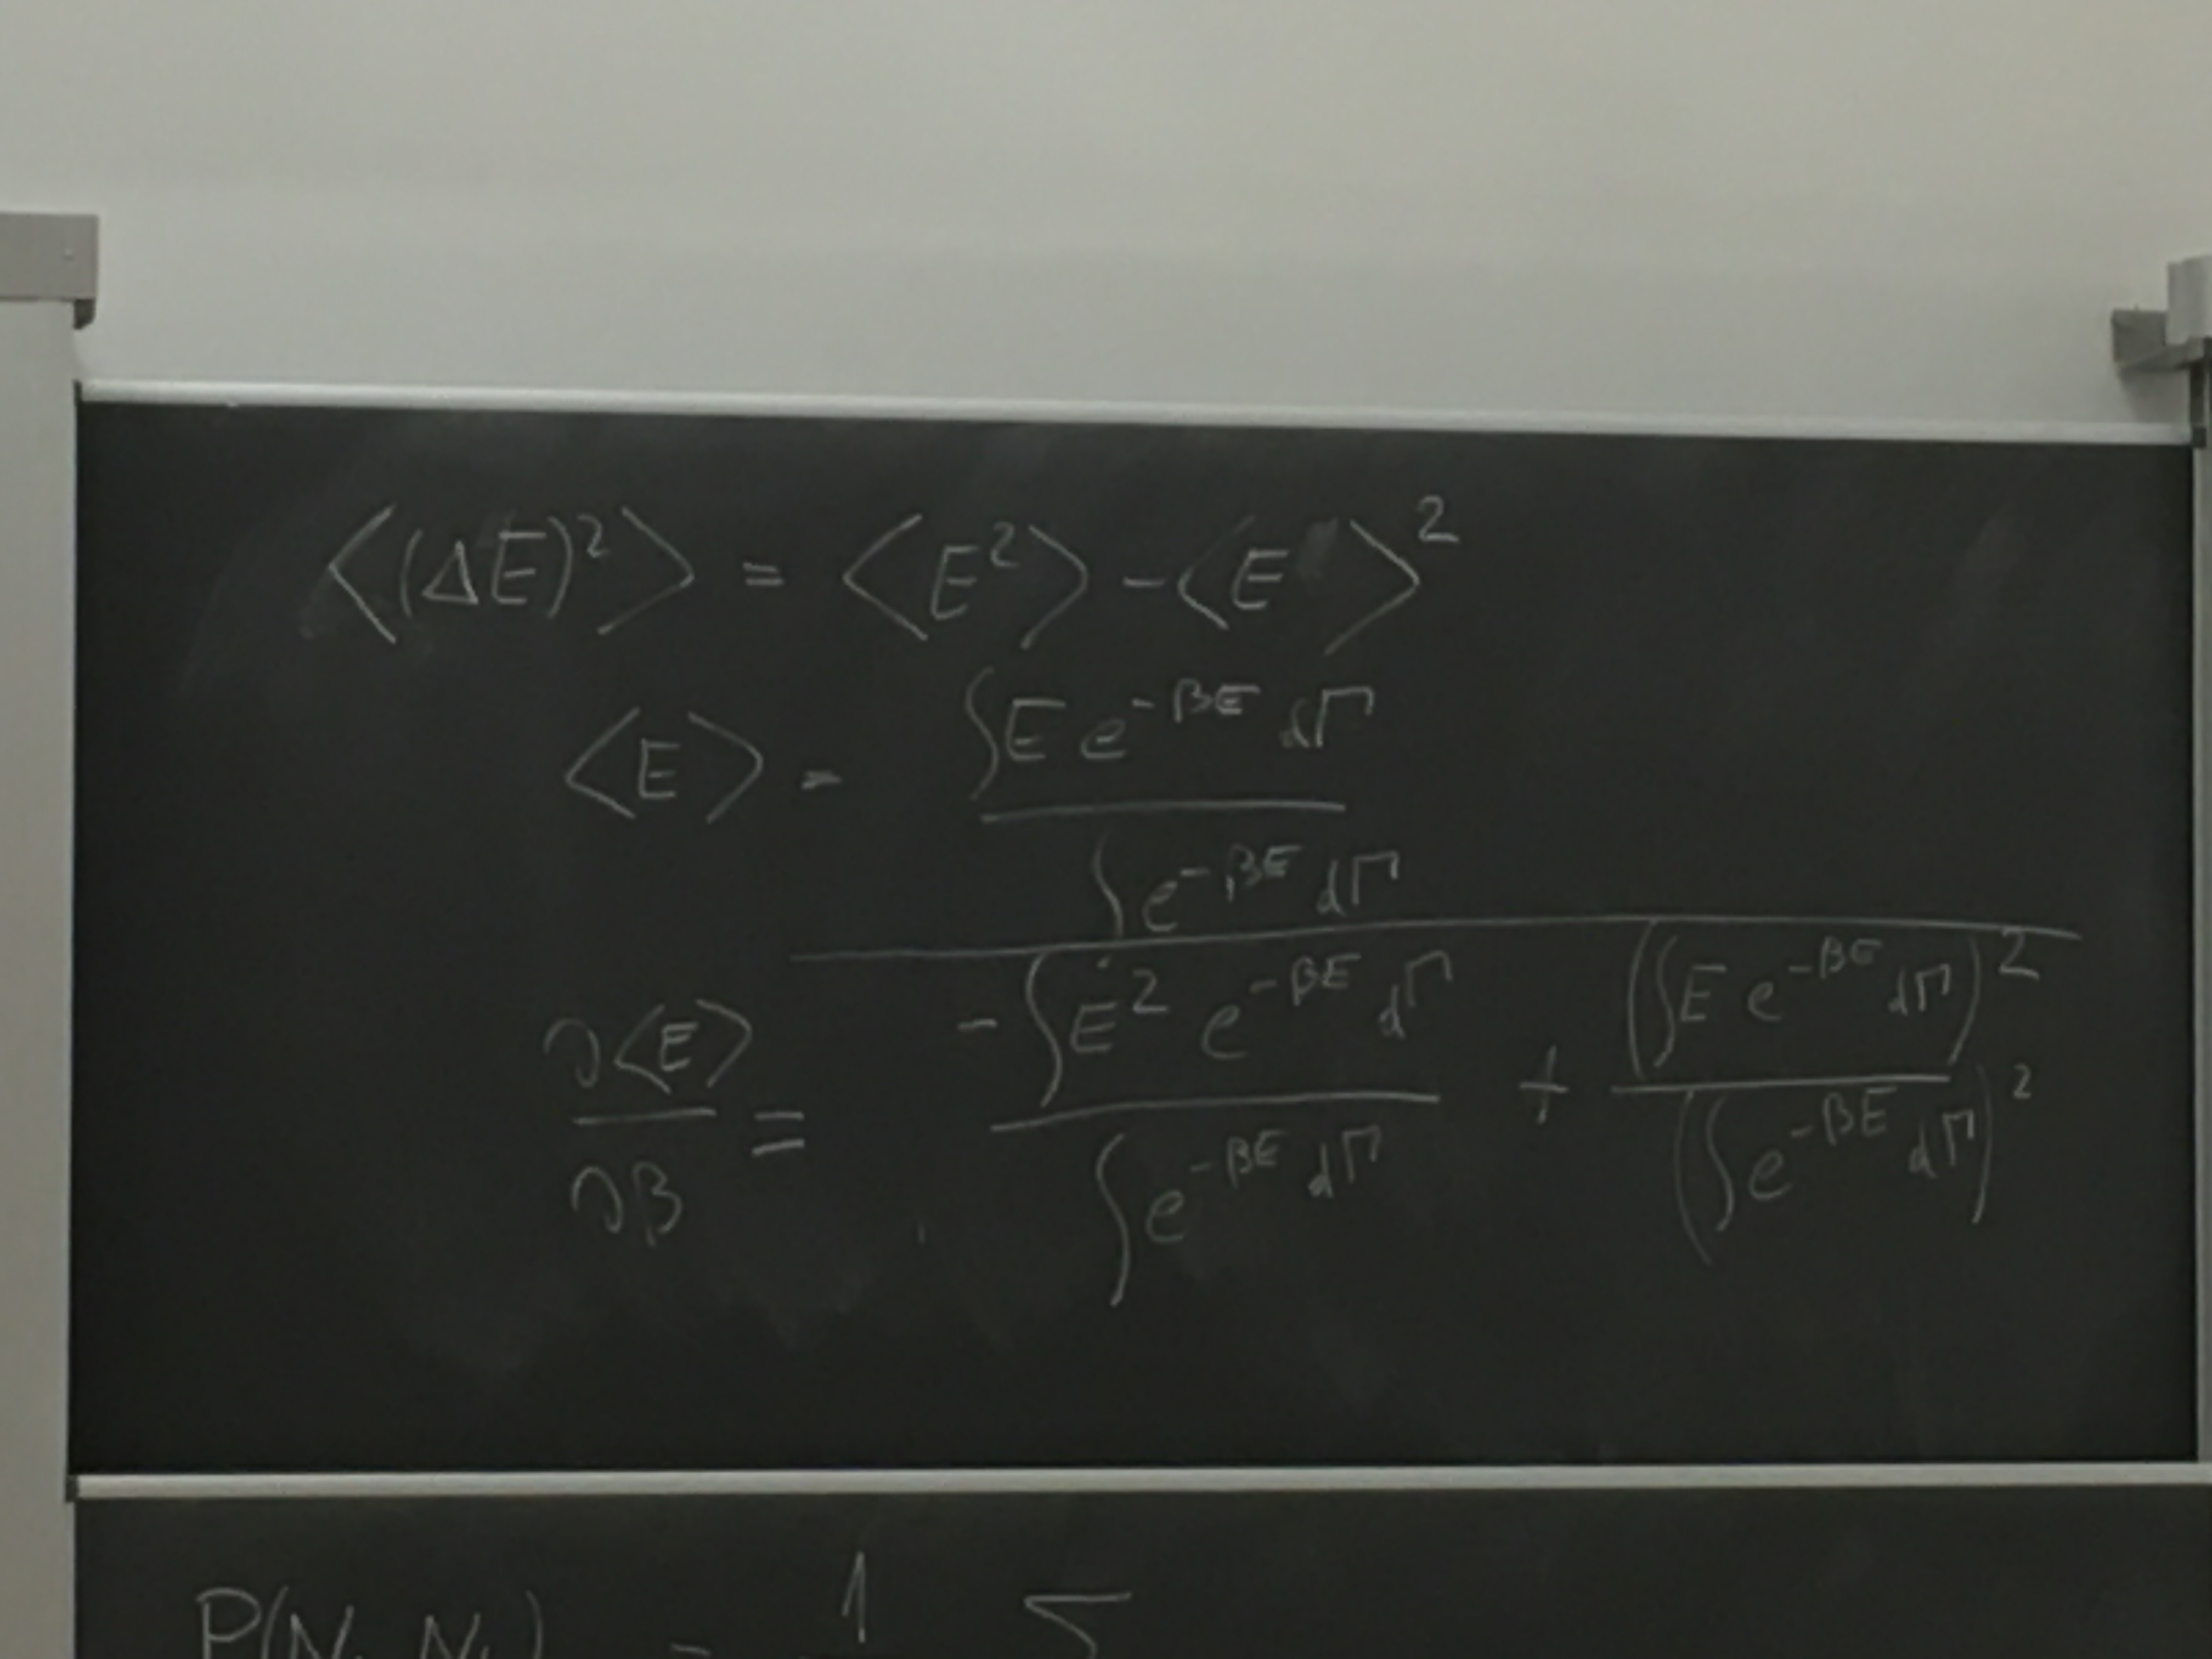
\includegraphics[width=\textwidth]{Wyk_8_Rys_2.JPG}
             \caption{Druga część}
             \label{fig:lec_8:do_przepisania_1.2}
         \end{subfigure}
        \caption{\com{Przepisz to do równań}}
        \label{fig:lec_8:do_przepisania_1}
     \end{figure}
\footnotetext{\com{Wklej Zdjęcie obliczeń aż do równoważności zespołów.}}

\section{Powrót to $\mu$}
\com{Wstaw rysunek z Goodnotes}

$$P(N_g, N_d) = \frac{1}{Z} \sum_{j: \mqty{N_g\text{ w }V_g\\N_d\text{ w }V_d}} e^{- \beta E_j} = \frac{Z(N_g, N_d,)}{Z}$$
Daje nam to: $Z(N_g, N_d) = Z_g(N_g)Z_d(N_d)$. Czy istnieje maksimum $P$?, tj.
\[
        \pdv{P}{N_g} \qc \pdv{\log P}{N_g}
\]
Tu jedna uwaga:
\[
    P_\text{mikro} = \frac{1}{\sum(E)} \qc P_\text{kanoniczne} = \frac{1}{Z} e^{-\beta \ev{E}}
\]
Daje nam to:
\begin{align*}
        S(E) &= k \log \sum(E)\qc P_M = e^{- S(E)/k} \implies P_K = P_M\\
        \frac{e^{- \beta \ev{E}}}{Z} &= e^{- \beta S(E)/k}
\end{align*}
Daje nam to:
\begin{equation}
    e^{- \beta (U - TS)} = Z
    \label{eq:lec_8:Z}
\end{equation}

Zdefiniujemy sobie tu taką wielkość:
\begin{equation}
    F = U - TS
    \label{eq:lec_8:energia_swobodna}
\end{equation}

Nazwiemy ją \subind{energią swobodną}{Energia Swobodna}.
\begin{align*}
    - \beta F &= \log Z\\
    F &= - k T \log Z\\
    \dd{F} &= \dd{U} - T \dd{S} - S\dd{T}\\
    \dd{S} &= \qty(\pdv{S}{U})_{VN} \dd{U} + \qty(\pdv{S}{V})_{UN}\dd{V} + \qty(\pdv{S}{N})_{VU}\\
    \dd{F} &= \dd{U} - T \qty(\frac{1}{T} \dd{U} + \frac{p}{T} \dd{V} - \frac{\mu}{T} \dd{N}) - S \dd{T} =\\
    &= - p \dd{V} - S \dd{T} + \mu \dd{N}\\
    \mu &= \qty(\pdv{F}{N})_{T, V}
\end{align*}
Wstawmy sobie to teraz dla naszej sytuacji dwóch zbiorników:
\begin{align*}
    \pdv{\log Z_g(N_g)}{N_G} - \pdv{\log Z_d(N_d)}{N_d} &= 0\\
    \color{BrickRed} \pdv{\log Z}{N} = -k T\mu\\
    \implies \mu_g = \mu_d
\end{align*}
Idąc dalej z tym rozumowaniem liczymy sobie:
\begin{align*}
    Z_g(N_g) &= \int e^{- \beta E_g\footnotemark} \dd{\Gamma_g} = {\color{BrickRed} E_g \approx mgh + U_w} = \qty(\frac{V_g}{\lambda^3} e^{-\frac{mgh}{kT}})^{N_g}/N_g! \implies\\
    \mu_g &\approx mgh + kT\log\frac{N_g \lambda^3}{V_g}\\
    \mu_d &\approx 0 + kT \log \frac{N_d \lambda^3}{V_d}\\
    % F = - kT \log Z &\qc \mu = (\pdv{F}{N) = -k T \pdv{\log Z}{N})
\end{align*}
\footnotetext{Energia grawitacyjna}
Duży $\mu$ - skłonność do dyfuzji.

Potencjał chemiczny to zmiana energii układu po dołożeniu nowej cząstki do niej.

\end{lecture}

% ----------------------------------------------------------------------
% Wykład 28.03.2022

\begin{lecture}{The return of Szymczak}
    \section{Podsumowanie tego co do tej pory osiągnęliśmy}
    \com{Zdjęcie}\\
    Stosujemy do Termodynamiki opis Statystyczny, tj. $\ev{A} = \sum_i A_i P_i$. Wyznaczanie $P_i$ jest trudne, ale wykonalne dla \emph{Stanów równowagi}.\\
    Dla \emph{układu izolowanego} w stanie równowagi:\\
    \begin{itemize}
        \item $P_i = \frac{1}{\sum_i}$
        \item $S = k \log \sigma$, gdzie $S$ - entropia
        \item Stan układu będziemy sobie definiować jako $S(E, V, N)$ i wiemy, że stanowi równowagi będzie odpowiadać stan makrostan realizujący największą liczbę mikrostanów.
    \end{itemize}
    Dostajemy takie równiania:
    \[
        -\frac{\mu}{T} = \qty(\pdv{S}{N})_{E,V}\qc\frac{1}{T} = \qty(\pdv{S}{E})_{V, N} \qc \frac{p}{T} = \qty(\pdv{S}{V})_{E, V}
    \]
    Czyli w szczególności różniczkę Entropii możemy zdefiniować jako:
    \[
        \dd{S} = \qty(\pdv{S}{U})_{V,N} \dd{U} + \qty(\pdv{S}{V})_{U,N}\dd{V} + \qty(\pdv{S}{N})_{V,U}
    \]
    Co dalej daje:
    \[
        T \dd{S} = \qty(\dd{E} + p \dd{V} - \mu \dd{N}) \implies
    \]
    \begin{equation}
        \dd{E} = \underbrace{T\dd{S}}_{\footnotemark} - \underbrace{p \dd{V}}_{\footnotemark} + \underbrace{\mu \dd{N}}_{\footnotemark}
        \label{eq:lec_9:1ZDN_rozniczkowa}
    \end{equation}
    \addtocounter{footnote}{-2}
    \footnotetext{Przepływ ciepła}
    \refstepcounter{footnote}
    \footnotetext{Praca wykonana przez siły zewnętrzne}
    \refstepcounter{footnote}
    \footnotetext{Wkład do zmiany energii od przepływu materii}
    Co jest \subind{pierwszą zasadą termodynamiki}{Zasada Termodynamiki!Pierwsza!Różniczkowa} w ujęciu różniczkowym.\\
    W ujęciu ogólnym jest daje to postać:
    \begin{equation}
        \Delta E = \underbrace{Q}_{\footnotemark} + \underbrace{W}_{\footnotemark}
        \label{eq:lec_9:1ZDN}
    \end{equation}
    \addtocounter{footnote}{-1}
    \footnotetext{Ciepło}
    \refstepcounter{footnote}
    \footnotetext{Praca wykonana przez siły zewnętrzne}
    Gdzie Równanie \eqref{eq:lec_9:1ZDN_rozniczkowa} możemy zapisać jedynie jeśli po drodze układ przechodzi przez kontinuum pośrednich stanów równowagi, tj. jest to \subind{proces odwracalny}{Proces!odwracalny}.
    Liczymy pracę w takiej zmianie. \com{Rysunki 1 i 2 z Goodnotes}.\\
    \wniosek Infintezymalna zmiana parametru wymuszającego zmienia kierunek procesu.\\
    Teraz wracamy do Równania \eqref{eq:lec_9:1ZDN_rozniczkowa}:
    \[
        \dd{E} = \dbar Q + \dbar W,qc \dbar Q = T\dd{S}\qc\dbar W = - p \dd{W}
    \]
    Piszemy $\dbar$ zamiast $d$ bo jest to różniczka niezupełna. Teraz, gdyby:
    \[
        \dd{Q} = \dd{E} + p \dd{V} \implies \dd{Q} = \qty(\pdv{Q}{E})_V \dd{E} + \qty(\pdv{Q}{V})_E \dd{V}
    \]
    Co dla gazu doskonałego, gdzie znamy zależność $p V \frac23 E \implies p(E, V) = \frac{2E}{3V} \implies \pdv{p}{E} = \frac{2}{3V}$ dało by nam:
    \[
        0 = \pdv{Q}{V}{E} \neq \pdv{Q}{E}{V} = \qty(\pdv{p}{E})_V =  \frac{2}{3V}
    \]
    Dlatego piszemy $\dbar$ a nie $d$. Jest tak dlatego, że jest to tzw. \subind{forma Pfaffla}{Forma Pfaffla}:
    \[
        \delta P = \sum_i f_i \dd{x_i}
    \]
    bo nie każda forma Pfaffla jest różniczką zupełną.
    \[
        \dd{f} = \sum_i \pdv{f}{x_i} (x_1 \dots x_n) \dd{x_i}
    \]
    $\dbar$ może stać się różniczką zupełną dla procesu adiabatycznego $(\dbar Q = 0)$, $\dd{E} = \dbar W$ i ona staje się różniczką zupełną dopiero po podzieleniu przez temperaturę:
    \begin{equation}
        \dbar Q = T \dd{S} \implies \frac{\dbar Q}{T} = \dd{S} \implies S_A - S_B = \int_A^B \frac{\dbar Q}{T}
        \label{eq:lec_9:zmiana_entropii}
    \end{equation}
    Kolejne co się pojawiło, to \emph{zespół kanoniczny}:
    \[
        P_i = \frac{e^{-\beta \overbrace{E_i}^{\footnotemark}}}{Z}
    \]
    \footnotetext{Energia mikrostanu}
    Gdzie $\beta = \frac{1}{kT}, Z = \sum_{m_i} e^{- \beta E_{m_i}}$ - suma statystyczna. Będziemy mogli sobie zdefiniować:
    \[
        U - TS = \underbrace{F}_{\footnotemark} = - k T \log Z
    \]
    \footnotetext{\subind{Energia Swobodna Helmholza}{Energia Swobodna!Helmholza}}
    \section{Gaz dokonały w zespole kanonicznym}
    Teraz policzymy sobie Gaz doskonały w zespole kanonicznym:
    \[
        Z = \int e^{- \beta \sum_i \frac{|\va{p}|^2}{2m}} \frac{\dd{p^{3N} } \dd{r^{3N}}}{h^{3N} N!} = \frac{V^N}{N! h^{3N}} \qty(2 \pi m k T)^{\frac{3N}{2}}
    \]
    Czyli idąć z $N \to \infty$:
    \[
        F = - k T \log Z = - k T \qty(N \log V - N \log N + N - 3 N \log h + \frac{3N}{2} \log (2 \pi m k) + \frac{3 N}{2} \log T)
    \]
    Co w granicy Termodynamicznej by nam wybuchło (bo jest to 
    \subind{wielkość intensywna}{Wielkość!Intensywna}), więc liczymy sobie energię swobodną na cząstkę (bo to już jest \subind{wielkością ekstensywną}{Wielkość!Ekstensywna}):
    \[
        f = \lim_{n\to\infty}\frac{F}{N} = - k T \qty(\log \underbrace{\frac{V}{N}}_{=v} + 1 - 3 \log h + \frac{3}{2} \log 2 \pi m k + \frac32 \log T)
    \]
    Teraz biorąc wzór $p \qty(\pdv{F}{V})_{T, N} = \qty(\pdv{f}{v})_{\Gamma} + \frac{kT}{v}$ dostajemy równanie stanu gazu doskonałego (\ind{Wzór Clapeyrona})
    \begin{equation}
        p v = k T \qc p V = N k T
        \label{eq:lec_9:clapeyron}
    \end{equation}
    Idziemy dalej. Wychodzimy od równania $\dd{U} = T \dd{S} - p \dd{V}$ co jest interpretacją ciepła i pracy w języku poziomów energetycznych. Wiemy, że $U = \ev{E} = \sum_i p_i E_i \gets$  suma po mikrostanach.
    \[
        \dd{U} = \sum_i\qty(\underbrace{\dd{E_i}}_{\footnotemark}p_i + \underbrace{E_i \dd{p_i}}_{\footnotemark})
    \]
    \addtocounter{footnote}{-1}
    \footnotetext{Zmiana energii poziomów}
    \refstepcounter{footnote}
    \footnotetext{Zmiana prawdopodobieństw obsadzenia poziomów $E_i$, $=T\dd{S}$}
    I teraz:
    \begin{align*}
        S &= - k \sum_i P_i \log P_i\qc\sum_i P_i = 1\qc \sum_i \dd{P_i} = 0\\
        \dd{S} &= - k \sum_i \dd{P_i} \overbrace{\log P_i}^{P_i = \frac{1}{Z} e^{-\beta E_i}} \underbrace{- k \sum_i P_i \frac{1}{P_i} \dd{P_i} }_{=0}\\
        T \dd{S} &= - T k \sum_i \dd{P_i} \qty(-\beta E_i \log Z) = \sum_i \dd{P_i}{E_i}
    \end{align*}
    Teraz wyobraźmy sobie, że poziomy się nie zmieniają, ale prawdopodobieństwa obsadzeń już tak (np. na skutek kontaktu z innym ciałem, przekazem ciepła) $\implies \dd{E_i} = 0 \to \dbar Q = \dd{U} \sum_i E_i \dd{p_i}$ co skutkuje przekazem entropii $\dd{S_e} = \frac{1}{T} \dbar Q = \frac{1}{T} \sum_i E_i \dd{P_i} $
\end{lecture}

% ----------------------------------------------------------------------
% Wykład 28.03.2022

\begin{lecture}{Twierdzenie Adiabatyczne}
Weźmy sobie:
\[
    E_{n_x n_y n_z} = \frac{\hbar^2\pi^2(n_x^2 + n_y^2 + n_z^2)}{2 m l^2}
\]
Spójrzmy sobie na poziomy energetyczne studni \com{Przerysuj ze zdjęcia}, to mamy: $L \to L'\qc\dd{P_i} = 0\qc\dd{E_i}\neq0$.
\begin{emph_box}{\subind{Twierdzenie Adiabatyczne}{Twierdzenie!Adiabatyczne}}
\emph{Twierdzenie Adiabatyczne}\textit{(mechanika kwantowa)}: Jeśli układ fizyczny był w stanie własnym Hamiltonianu $H(0)$ określonym liczbami kwantowymi $n$, to jeśli tylko $H$ zmienia się dostatecznie wolno, to układ pozostaje w stanie własnym Hamiltonianu $H(t)$ scharakteryzowanego tym zespołem liczb kwantowych.
\end{emph_box}

Widzimy, że w związku z tym:
\begin{align*}
    U &= \sum_i E_i P_i\qc S = ik\sum_i P_i \log P_i\\
    \dd{U} &= \sum_i\qty(\underbrace{\dd{E_i}P_i}_{\footnotemark} + \underbrace{E_i\dd{P_i}}_{\footnotemark})\qc\dd{S} = \frac{1}{T} \sum_i \dd{P_i}E_i
\end{align*}
\addtocounter{footnote}{-1}
\footnotetext{Praca}
\refstepcounter{footnote}
\footnotetext{$T\dd{S}$ - Ciepło}
Czy to nie oszustwo?
Bo widzimy, że na początku mamy:
\[
    p_n^i = e^{-\beta \frac{\hbar^2 \pi^2 n^2}{2 m L^2}}
\]
\[
    p_n^f = e^{-\beta' \frac{\hbar^2 \pi^2 n^2}{2 m (L')^2}}
\]

\textit{Jeśli to Pana niepokoi, to może Pan wyłączyć mózg $\sim$ P. Szymczak 31.03.2022}
Gdzie $\beta = \frac{1}{kT}, \frac{\beta}{L^2} = \frac{\beta'}{(L')^2} \implies T L^2 = T' (L')^2 \implies L = V^{\frac13} \implies T V^{\frac23} = const.$\\
Czyli po wstawieniu tego wyniku do Równania Clapeyrona dostajemy $pV = NkT \implies T = \frac{pV}{Nk}$ Co też daje nam:
\[
    pV^{\frac53} = const.
\]
Jest to \emph{równanie adiabaty dla gazu doskonałego}.\\
Z tego też widać, że w rozumieniu fizyki statystycznej, \emph{adiabatycznie}, to znaczy bez wymiany ciepła z otoczeniem, a niekoniecznie nieskończenie wolno, co jest rozumieniem kwantowym.
Z tego wynika nam dalej:
\begin{enumerate}
    \item $\dbar W = \dd{U} = \sum_i P_i\dd{E_i} \gets$ kwazistatyczne, adiabatyczne (statystycznie) sprężanie układu
    \item $\dd{E_i} = 0 \qc \dd{U} = \dbar{Q} = \sum_i E_i \dd{P_i} \qc S_e = \frac{1}{T} \sum_i E_i \dd{P_i}$, gdzie $S_e$ to zewnętrzna zmiana entropii.
    \item Jeśli zmiana poziomów energetycznych nie następuje bardzo wolno, to cząstni mogą zmieniać stan ("spadanie kur z grzęd w tej studni nieskończonej"), przy czym prawdopodobieństwo przejśćia $i \to j$ wynosi:
    \[
        H' = H_o + V'\qc \tilde{P_{ij}} = \mel{\Psi_i}{V'}{\Psi_j} = \tilde{P_{ji}}
    \]
    Gdzie $v'$ jest zaburzeniem.
\end{enumerate}
Teraz patrzymy na prawdopodobieństwo obsadzenia stanu po zaburzeniu, $P_i'$.
\begin{align*}
    P_i' &= \sum_j \tilde{P_{ij}} P_j\\
    \dd{P_i} = P_i' - P_i = \sum_j \tilde{P_{ij}}P_j - P_i = \sum_j \tilde{P_{ij}}P_j - \sum_j \tilde{P_{ij}}P_i = \sum_j \tilde{P_{ij}}(P_j - P_i)
\end{align*}
W związku z tym zmiana energii:
\[
    \sum_i E_i\dd{P_i} = \sum_{i,j} \tilde{P_{ij}} E_i (P_i - P_j) = \sum_{i,j} \tilde{P_{ji}} E_j (P_i - P_j) = \frac12\qty(\sum_{ij} \tilde{P}_{ij} E_i (P_j-P_i) - \tilde{P}_{ji} E_j (P_j - P_i))
\]
\[
    \sum_i E_i \dd{P_i} = \frac12\sum_{ij}\tilde{P}_{ij}(E_i-E_j) (P_i-P_j) >0 
\]
I dlaczego to jest dodatnie? Ponieważ $p \sim e^{-\beta E_i}$. Czyli:
\[
    \dd{S_int} = \frac{1}{2T} \sum_{ij} \tilde{P}_{ij} (E_i-E_j) (P_i-P_j) 
\]
Zatem zmienia się energia, bez wymiany ciepła z otoczeniem. \\
Daje nam to też \subind{Drugą Zasadę Termodynamiki}{Zasada Termodynamiki!Druga}.\\
Zbierając te wyniki w całość dostajemy, że $\sum_i E_i \dd{p_i}$ można dostać w wyniku przekazu ciepła z otoczeniem, lub w wyniku przeprowadzenia nagłego nieodwracalnego procesu. Stąd wynika:
\begin{equation}
    \dd{S} = \dd{S_{int}} + \dd{S_{ext}} = \frac{\dbar Q}{T} + \underbrace{\dd{S_{int}}}_{\footnotemark}
\end{equation}
\footnotetext{Związane z nieodwracalnością, nieadiabatycznością (Mech.Kwant.) procesu lae nie przekazem ciepła}
Daje nam to \emph{Drugą Zasadę Termodynamiki}
\begin{emph_box}{\subind{Druga Zasada Termodynamiki}{Zasada Termodynamiki!Druga}}
    Biorąc za $S$ Entropię Gibbsa:
    \begin{equation}
        \dd{S} \geq \frac{\dbar Q}{T}
    \end{equation}
    Co dla układu izolowanego ($\dbar Q = 0$) daje nam:
    \begin{equation}
        \dd{S} \geq 0
    \end{equation}
    Czyli inaczej mówiąc, Entropia układu izolowanego nigny nie maleje, nie zmienia się w procesach odwracalnych, a w nieodwracalnych rośnie.
\end{emph_box}

\section{Zespół wielki kanoniczny}
Zespół wielki kanoniczny, to taki, gdzie układ może z otoczeniem wymieniać nie tylko ciepło ale i cząstki. \com{Wstaw rysunek}
Czyli jego własności są takie. Biorąc $E_1, N_1, V_1$ jako stan układu, a $E_2, N_2, V_2$ stan otoczenia mamy $N_1 + N_2 = const.$ a $E_1 + E_2 = const.$
Własności:
\begin{enumerate}
\item Dla całego układu $(1+2)$ obowiązuje rozkład mikrostanów
\[
    \rho(\Gamma^{(1)}, \Gamma^{(2)}) = \frac{1}{\omega(E, N, V)} \delta(E - E_1(\Gamma^{(1)}_1 N_1) - E_2(\Gamma^{(2)}_1 N_2))
\]
\item Nas ciekawią tylko prawdopodobieństwa poszczególnych mikrostanów układu $(1)$ bez względu na to co dzieje się w $(2)$.
\[
    \rho_1(\Gamma^{(1)}) = \int \dd{\Gamma_2} \rho(\Gamma^{(1)}, \Gamma^{(2)}) = \int \dd{\Gamma_2} \frac{1}{\omega(E, V, N)} \delta(E- E_1-E_2)
\]
\begin{equation}
    \rho(\Gamma^{(1)}) = \frac{1}{\omega(E, V, N)} \omega_2(E - E_1(\Gamma^{(1)}_1 N_1), V_2, N-N_1)
    \label{eq:lec_10:cos_1}
\end{equation}
Rozwińmy log $\omega_2$:
\[
    \log \omega_2(E- E_1, V_2, N-N_1) = \log \underbrace{\omega_2(E, V_2, N)}_{\frac{1}{k}S_2(E, V_2, N)} - \underbrace{\frac{1}{k}\pdv{k \log \omega_2}{E}E_1}_{\pdv{S}{E} = \frac{1}{T}} - \pdv{\log \omega_2}{N}N_1
\]
Pamiętając o tym, że $S = k \log \omega$:
\[
    \log \omega_2 (E-E_1, V_1, N-N_1) = \frac{1}{k} S_2 (E, V, N) - \beta E_1 + N \beta N_1
\]
Gdzie $\beta = \frac{1}{kT}$
\[
    \omega_2 (E-E_1, V_2, N-N_1) = A e^{-\beta (E_1 - \mu N_1)}
\]
Gdzie wielkość $z = e^{\beta \mu}$ nazwiemy \emph{aktywnością}. Wstawiamy teraz do równania \eqref{eq:lec_10:cos_1}, biorąc $\Xi(T, V, \mu) = \sum_N \int e^{-E - \mu N} \dd{\Gamma_N}$:
\[
    \rho_1(\Gamma^{(1)}) = \frac{1}{\Xi} e^{-\beta E_1 - \mu N} = \frac{1}{\Xi}z^N_1 e^{-\beta E_1}
\]
Stała normalizacyjna w zespole daje nam zwykle najwiecej informacji o układzie, więc spójrzmy sobie na stałą $\Xi$. Dostajemy ją jako:
\[
    \Xi(T, V, \mu) = \sum_{N=0}^{\infty} Z^N \int e^{-\beta E(\Gamma_N, V)} \dd{\Gamma_N}
\]
Teraz porównując sobie zespół kanoniczny z wielkim kanonicznym:
\[
    \frac{e^{-\beta \ev{E}}}{z} = \frac{-\beta \ev{E} - \mu \ev{N}}{\Xi}
\]
Daje nam to dalej:
\[
    z e^{\beta \mu \ev{N}} = \Xi \implies \log z + \beta \mu \ev{N} = \log \Xi
\]
Czyli jest to:
\[
    F - \mu \ev{N} = - k T \log \Xi \equiv \Omega(T, V, \mu)
\]
Wielkość $\Omega$ to \ind{Wielki podencjał termodynamiczny}
\end{enumerate}


\end{lecture}

\tableofcontents

\listoffigures

\printindex

% ----------------------------------------------------------------------------------------------
% Appendix

\begin{center}
    \chapter*{Załączniki}
\end{center}

\appendix
\setcounter{table}{0}
\captionsetup[table]{name=Załącznik}
\captionsetup[figure]{name=Załącznik}
\captionsetup[section]{name=Lecture}

\chapter{Długaśne wyprowadzenia wzorów}

\section{Lecture 5}

\begin{figure}[!ht]
    \centering
    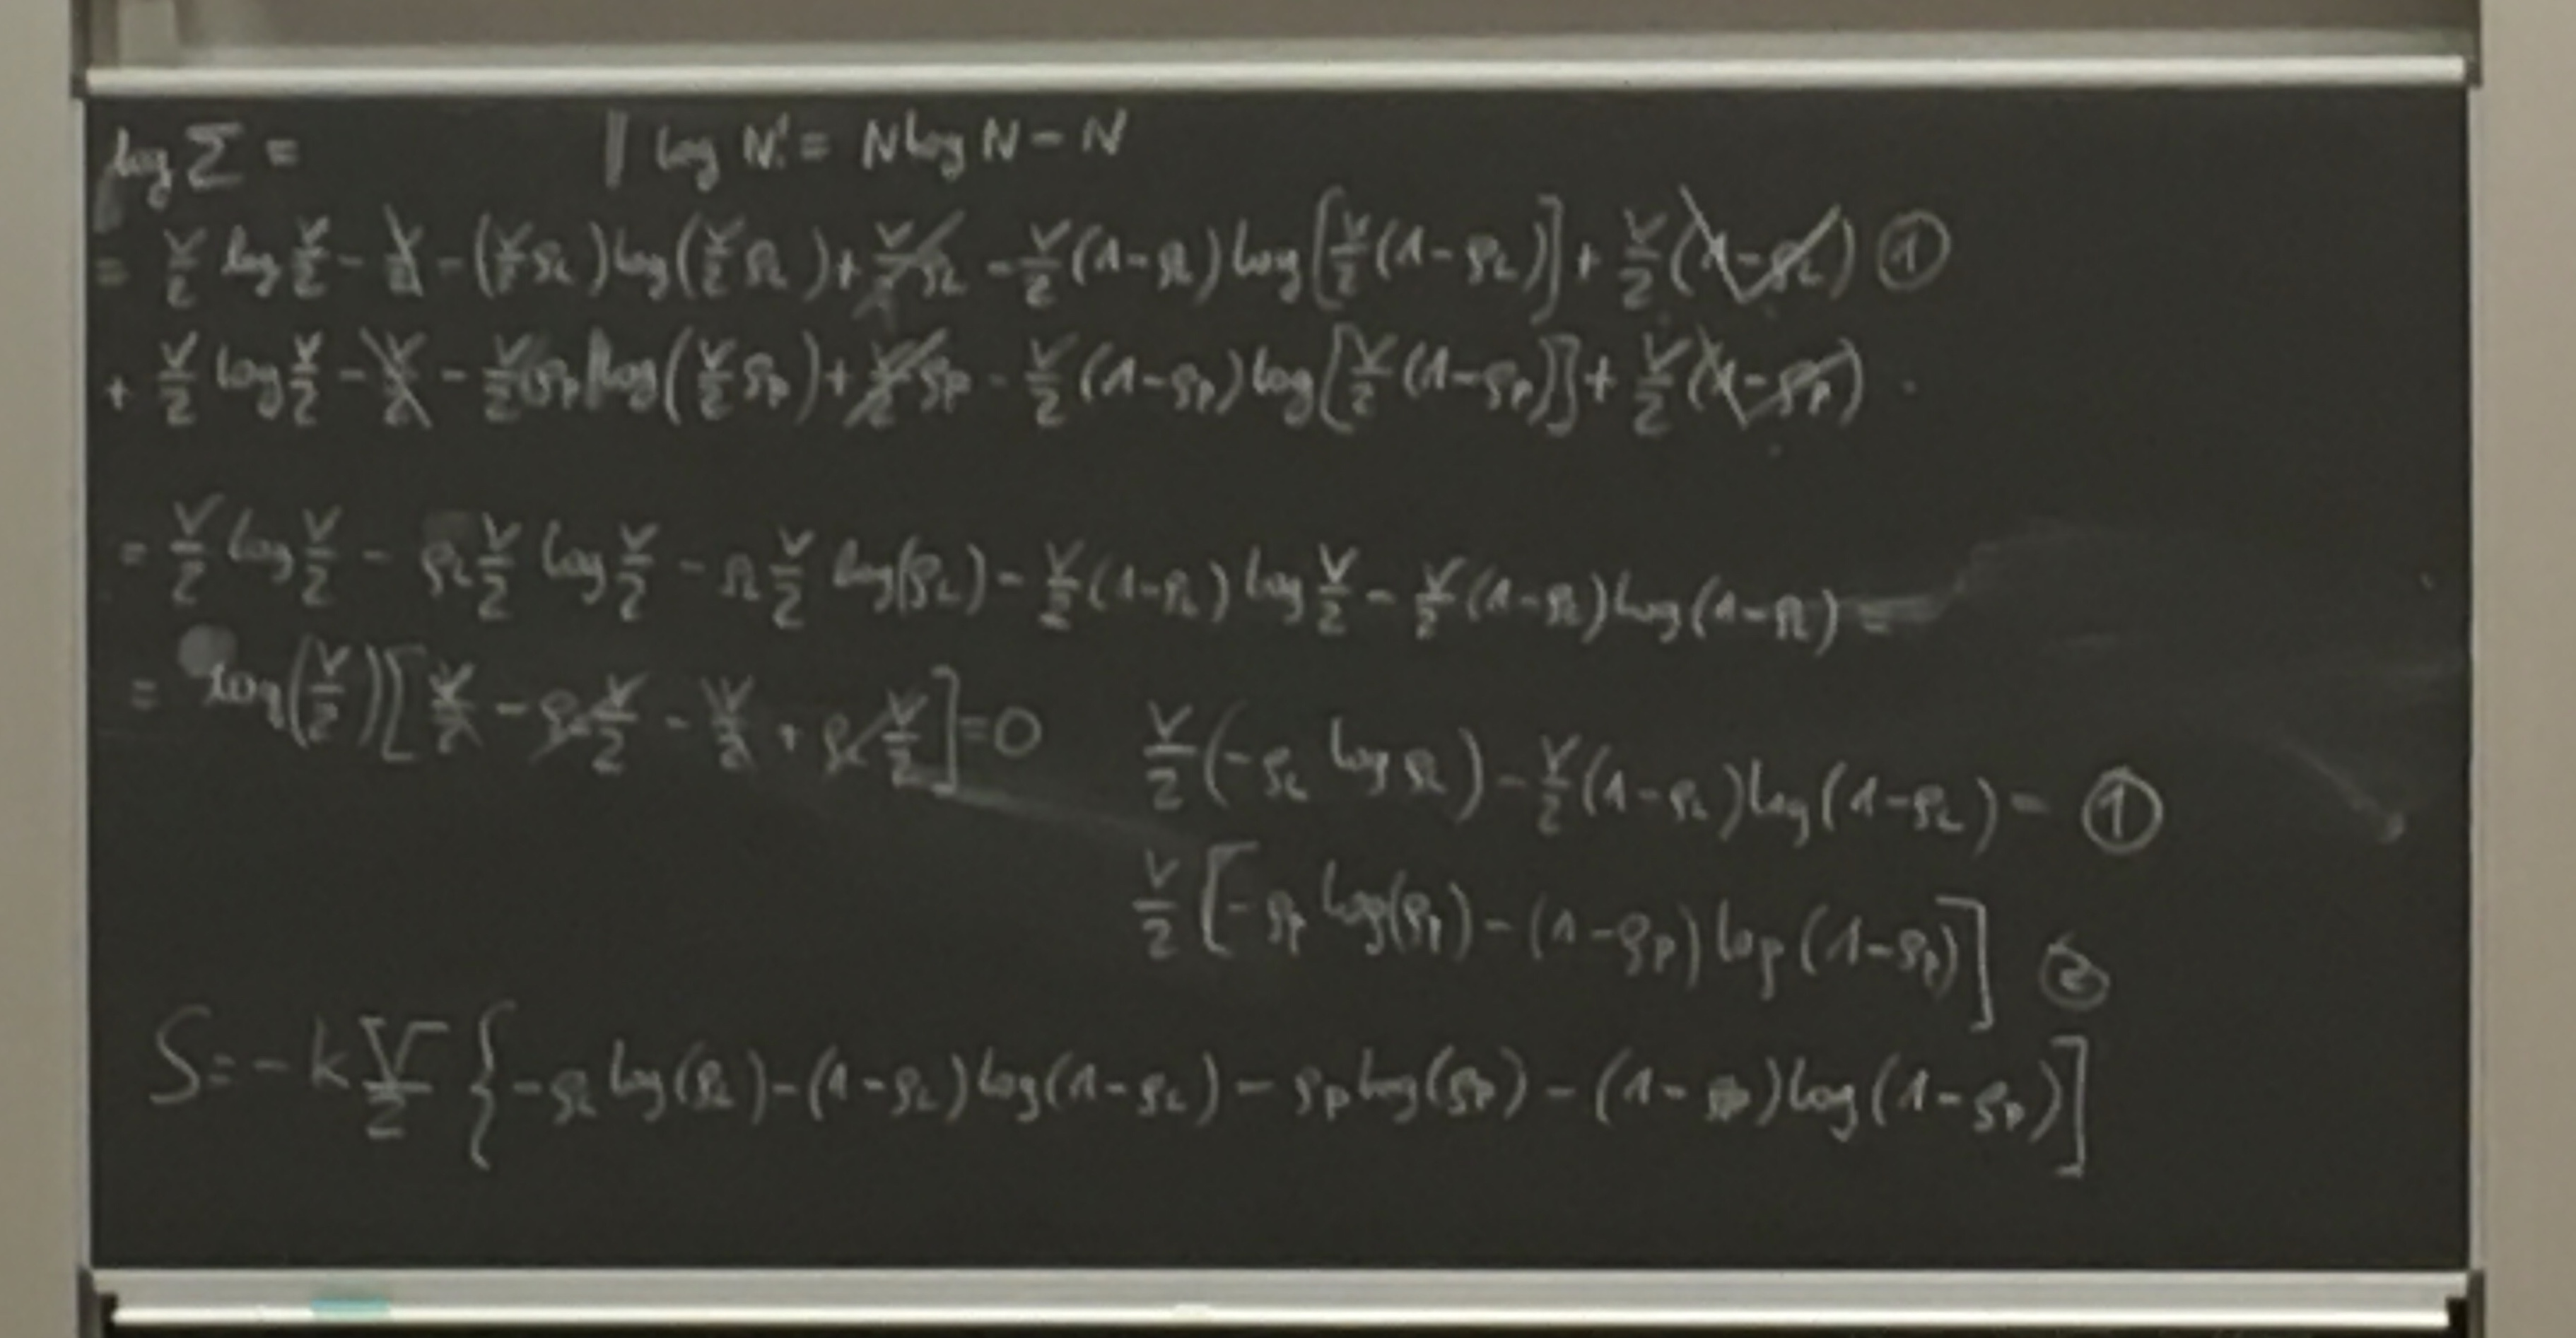
\includegraphics[width=\linewidth]{Wyk_5_Rys_2.JPG}
    \caption{Wyprowadzenie wzoru na maksymalizację entropii}
    \label{fig:lec_5:app:maksymalizacja_entropii}
\end{figure}


\begin{figure}[!ht]
    \centering
    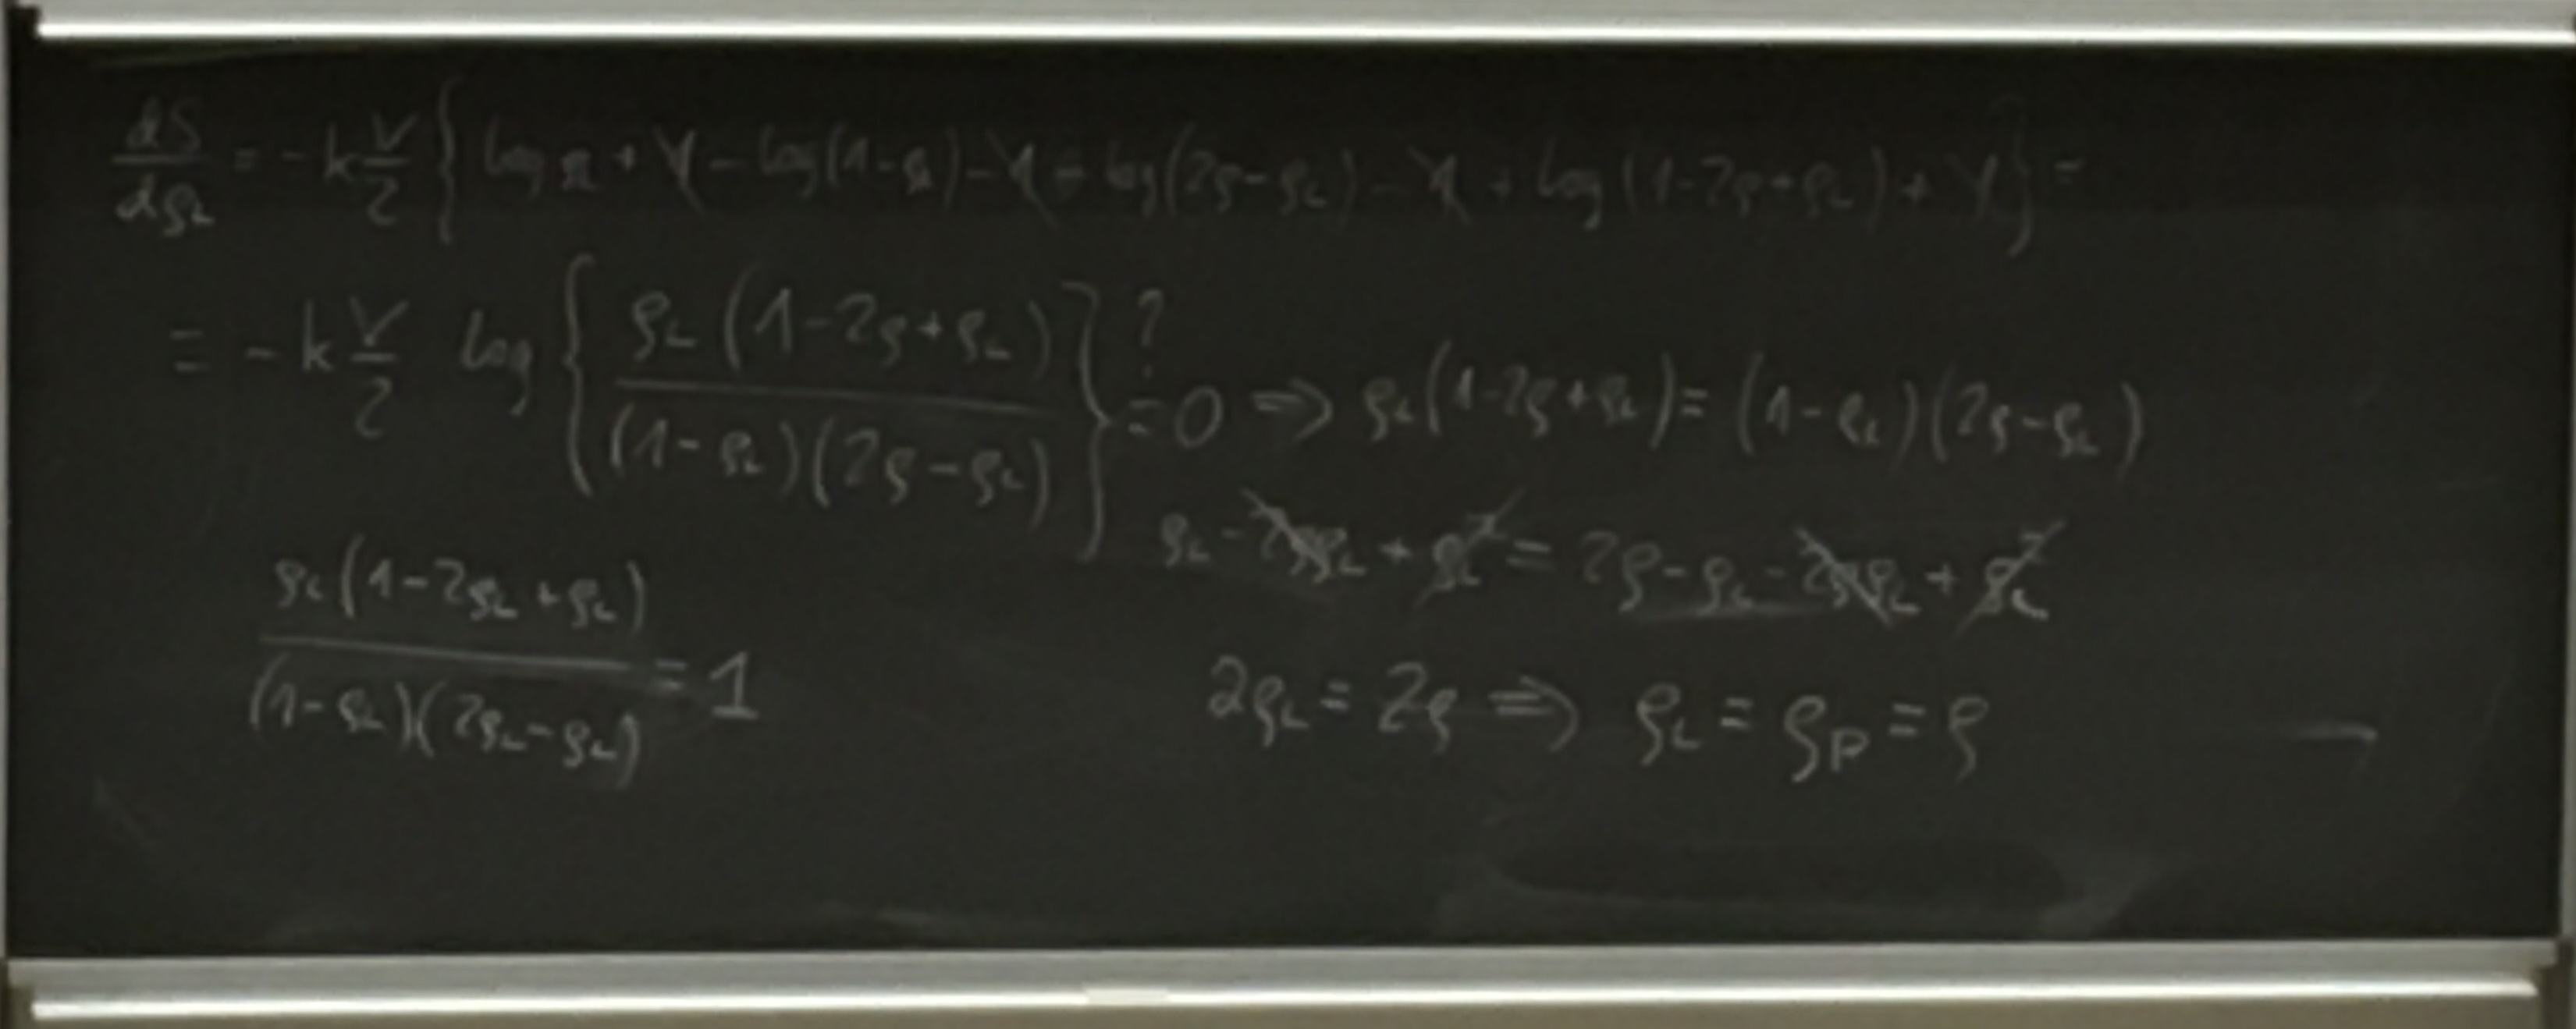
\includegraphics[width=\linewidth]{Wyk_5_Rys_3.JPG}
    \caption{Wyprowadzenie wzoru na maksymalizację entropii cz.2}
    \label{fig:lec_5:app:maksymalizacja_entropii_2}
\end{figure}

\chapter{Przydatne wzorki}

\emph{Wzór Stirlinga}
\begin{equation}
    \log m! \approx \frac12 \log 2 \Pi + (m+1) \log m - m \dots
    \label{eq:app_wzory:stirling}
\end{equation}

\linediv

\emph{Entropia}

\begin{itemize}
    \item $G_m$ - liczba mikrostanów odpowiadającuch makrostanom $m$, $G_m = \mqty(N \\ m)$
    \item $P_m(t)$ - prawdopodobieństwo makrostanu ($m$ pcheł na Azorze)
    \item $p_i(t)$ - prawdopodobieństwo mikrostanu, $p_i (t) = \frac{P_m(t)}{G_m(t)}$\footnote{Wszystkie mikrostany odpowiadające makrostanom $m(i)$ są równoprawdopodobne.}
\end{itemize}


\emph{Entropia Boltzmanna}
\begin{equation}
    S_B = k \log G_m
    \label{eq:app:entropia_boltz}
\end{equation}

\emph{Entropia Gibbsa}
\begin{equation}
    S_G = - k \sum_i p_i\footnote{Prawdopodobieńśtwo wystąpienia mikrostanu} \log p_i
    \label{eq:app:entropia_gibbs}
\end{equation}

\linediv

\emph{Rozkłady}

\emph{\subind{Rozkład Cauchy'ego}{Rozkład!Cauchy'ego}}
\begin{equation}
    P_x = \frac{1}{\pi \gamma} \qty[\frac{\gamma^2}{(x-x_0)^2 + \gamma^2}]
    \label{eq:app:rozklad_cauchy}
\end{equation}

\begin{itemize}
    \item $P_x$ - Rozkład gęstości prawdopodobieństwa
    \item $\gamma$ - Parametr skali (np. na ćwiczeniach odległość działa od ekranu)
    \item $x_0$ - przesunięcie peaku względem środka U.W.
\end{itemize}

\emph{\subind{Rozkład Maxwella}{Rozkład!Maxwella}}
\begin{equation}
    P(v) = 4 \pi v^2 \qty(\frac{m}{2 \pi k T})^{\frac32} e^{-\frac{\frac12 m v^2}{k T}}
    \label{eq:app:rozklad_maxwell_v}
\end{equation}

\begin{equation}
    P(E) = 2 \sqrt{\frac{E}{\pi}} \qty(\frac{1}{k T})^{\frac32} e^{-\frac{E}{kT}}
    \label{eq:app:rozklad_maxwell_E}
\end{equation}

\begin{itemize}
    \item $P(v)$ - Rozkład Maxwella w funkcji prędkości cząsteczek
    \item $P(v)$ - Rozkład Maxwella w funkcji Energii cząsteczek
    \item $\gamma$ - Parametr skali (np. na ćwiczeniach odległość działa od ekranu)
    \item $x_0$ - przesunięcie peaku względem środka U.W.
\end{itemize}


\end{document}